\documentclass[3p,12pt]{elsarticle}

\usepackage{amssymb}
\usepackage{amsmath}
\usepackage{url}
\usepackage{float}
\usepackage{subcaption}
\usepackage{booktabs}
\usepackage{etoolbox}
\AtBeginEnvironment{tabular}{\def\baselinestretch{1}\selectfont}
\usepackage[section]{placeins}
\pretocmd{\subsection}{\FloatBarrier}{}{}
\pretocmd{\subsubsection}{\FloatBarrier}{}{}
\renewcommand{\thesubsubsection}{\thesubsection.\alph{subsubsection}}
\renewcommand{\topfraction}{0.90}
\renewcommand{\bottomfraction}{0.70}
\renewcommand{\textfraction}{0.10}
\renewcommand{\floatpagefraction}{0.75}
\emergencystretch=3em

\newcommand{\MITgcm}{\textsc{MITgcm}}
\newcommand{\FNO}{FNO}
\newcommand{\Sforced}{S_{\mathrm{forced}}}

\begin{document}

\begin{frontmatter}

\title{Forward-response supervision of a stable double-gyre Fourier neural operator}

\author[ucsb]{Maxime Jalabert}
\ead{mjalabert@ucsb.edu}
\author[jpl]{Ian Fenty}
\author[jpl]{Ou Wang}

\affiliation[ucsb]{organization={University of California, Santa Barbara}}
\affiliation[jpl]{organization={NASA Jet Propulsion Laboratory}}

\begin{abstract}
A Fourier neural operator (\FNO{}) emulator of a \MITgcm{} double-gyre
configuration can forecast the ocean state well while its reverse-mode gradient
bears almost no resemblance to the ocean model's true adjoint. This report
presents a matched pair of models trained to test whether that gap can be closed
using forward information alone: a \emph{control} model trained with eight-term forecast objective, and a \emph{response} model
that is identical in every respect except for one added loss term matching the
emulator's finite-difference perturbation response to \MITgcm{}'s. No adjoint
quantity, from either side, enters training or model selection. Both arms are
compared forward, over a 2{,}000-day held rollout, and in the adjoint, against
\MITgcm{} differentiated by TAF, at three sea-surface-height targets spanning the
basin, two cost functionals, and leads of 10, 30 and 90 days. The forward
comparison shows the two arms are follow the same evolution out to roughly two years and
then separate, with the response arm drifting past climatology
where the control arm stays close to it. The adjoint comparison shows the
response term reliably reduces the sensitivity error --- relative $L_2$ falls in
every one of the 18 (target, objective, lead) cells reported here, by up to
32\% --- but does not repair its structure: pattern correlation against the true
adjoint stays between $-0.15$ and $+0.18$ everywhere, for both arms. The one
exactly known mode, the conserved basin-mean sea level, is damped by both models
at a near-constant factor of $0.38$ per ten-day call. Response supervision
therefore corrects sensitivity magnitude without recovering sensitivity
structure.
\end{abstract}

\end{frontmatter}

\section{Introduction}
\label{sec:intro}

\MITgcm{} and models like it solve the discretized primitive equations directly
and are accurate, but expensive: a single integration at useful resolution can
take days of wall-clock time, and the ensembles that data assimilation,
uncertainty quantification and sensitivity studies all require multiply that
cost by however many members are needed. Data-driven emulation offers a
shortcut. Rather than solving the equations, an emulator learns a single Markov
map from the ocean state at time $t$ to the state one interval later,
$x(t)\mapsto x(t+\Delta t)$, from a library of \MITgcm{}
trajectories; once trained, that map can be applied autoregressively to produce
forecasts, and ensembles of forecasts, at a marginal cost far below the original
solver's. Fourier neural operators are particularly well suited to this:
\FNO{}s naturally learn global interactions between spatial fields, whereas
traditional neural networks require architectural mechanisms such as
convolutions to exploit spatial structure. Bire et
al.~\cite{Bire2025} trained one to emulate the fine, turbulent \MITgcm{}
double-gyre configuration autoregressively and showed it stays stable and
skillful over rollouts of thousands of days, far beyond the lead times used in
training.

Forecast skill is not the only property such an emulator needs, and for the
applications that motivate building one in the first place it is not even the
most important one. Data assimilation, parameter estimation and sensitivity
analysis all depend on the \emph{derivative} of the flow map,
$\partial J/\partial x_0$, the sensitivity of some later cost functional
$J$ to the initial state --- not on the map itself. This derivative, computed by
the adjoint operator, reveals which earlier locations and variables a later
quantity of interest actually depends on; it is the object underlying
four-dimensional variational data assimilation, observing-system design, and
optimal control in ocean and climate models generally. Nothing in a
forecast-only training objective constrains this derivative directly, only the
states it happens to be evaluated on, so a model can reproduce trajectories well
while its derivative is wrong. This is not a hypothetical concern. Ruiz~\cite{Ruiz2025}
built a reverse-mode adjoint pipeline for Samudra~\cite{Dheeshjith2025}, a fast
neural ocean emulator with genuinely strong forward skill, and compared it
directly against \MITgcm{}'s: Samudra's sensitivities were internally
self-consistent but diffused far faster than \MITgcm{}'s, alternated sign on
adjacent grid cells where \MITgcm{}'s stayed spatially coherent, and showed no
trace of the westward-propagating Rossby-wave signal that \MITgcm{}'s adjoint
carries clearly at long lag. A follow-on internship at JPL of Mousavi~\cite{Mousavi2025},
motivated explicitly by that result, abandoned differentiating the forward
emulator altogether and instead trained a separate network to emulate the
adjoint recursion itself --- a tacit acknowledgment that a good forward
emulator's own derivative could not be trusted directly.

JPL's specific advantage in pursuing this question further is access to a
mature, TAF-differentiated \MITgcm{} adjoint, verified against finite
differences and used routinely for ocean state estimation. That reference
adjoint makes a direct, apples-to-apples comparison possible: differentiate a
trained emulator in reverse mode, differentiate \MITgcm{} through TAF over the
identical trajectory and cost functional, and compare the two sensitivity maps
cell by cell rather than relying on qualitative plausibility checks alone.

The scientific question this line of work poses is therefore simple to state:
does a good forward emulator also learn the correct sensitivities? On the
evidence assembled so far --- Samudra against \MITgcm{}, the dedicated adjoint
surrogate's own limitations at long lag, and this project's own production
\FNO{} --- the answer is that it is not guaranteed. That diagnosis suggests a targeted remedy. A Jacobian-vector product is, to
leading order, a forward finite difference; a large enough set of \MITgcm{}
perturbation experiments therefore constrains the emulator's Jacobian using only
forward integrations, with no adjoint code, no TAF output, and no risk of
training on the very quantity the study is meant to test. This report presents
the two models that test that idea, both trained from random initialization on
the weakly turbulent S0 double gyre:

\begin{itemize}
\item the \textbf{control model} (arm B, \texttt{model\_c\_adjoint\_faithful\_nominal\_control\_v1}),
trained with the project's existing eight-term forward objective and nothing else;
\item the \textbf{response model} (arm C, \texttt{model\_c\_adjoint\_faithful\_response\_v1}),
identical in architecture, data, split, optimizer, schedule and objective, plus
exactly one additional loss term that matches signed forward perturbation
responses against \MITgcm{}.
\end{itemize}

Section~\ref{sec:method} describes the two models and the design choices behind
them. Section~\ref{sec:setup} states the evaluation protocol. Section~\ref{sec:results}
reports the forward comparison and then the adjoint comparison at three targets and
two cost functionals. Sections~\ref{sec:discussion} and~\ref{sec:conclusion}
interpret the outcome.

\section{Methodology}
\label{sec:method}

\subsection{Problem formulation}
\label{sec:formulation}

The emulator is a single Markov operator advancing the full prognostic ocean
state ten days,
\[
F_\theta:\;[\,x_t,\,S\,]\;\longmapsto\;x_{t+10},
\]
on the \MITgcm{} \texttt{tutorial\_baroclinic\_gyre} configuration at one degree
($62\times62$ cells, $15^\circ$--$75^\circ$N), deliberately coarser and less
turbulent than the $0.25^\circ$ configuration of Bire et al.~\cite{Bire2025}: in
a weakly turbulent regime trajectories do not diverge chaotically
(Section~\ref{sec:setup}), so a mismatch between the emulator's and
\MITgcm{}'s Jacobians can be attributed to the emulator itself rather than to
sensitive dependence on initial conditions, making this a cleaner first
testbed before attempting the same comparison in Bire et al.'s fully turbulent
regime. The state
$x\in\mathbb{R}^{46\times62\times62}$ holds fifteen vertical levels each of zonal
velocity $U$, meridional velocity $V$ and potential temperature $\Theta$, plus
the free surface $\eta$; $S$ holds five static physical fields (wind stress, wet
mask, Coriolis parameter, grid spacing, SST relaxation target) and a two-channel
position encoding. Keeping the state closed --- every prognostic variable, no
diagnostic reductions --- is what makes the Jacobian of $F_\theta$ a candidate
tangent-linear operator at all; a reduced state would not support one. Training
and inference are done in pointwise-normalized coordinates,
\[
\mathcal N(x)_c(y,x) \;=\; \frac{x_c(y,x)-\mu_c(y,x)}{\sigma_c(y,x)},
\]
with $\mu,\sigma$ computed from training days only and land set to zero. A
forecast to lead $T=10k$ days is $k$ self-fed applications of $F_\theta$.

Writing $M_k$ for the true \MITgcm{} flow map over $k$ ten-day steps and
$F_{\theta,k}$ for the emulator's, forecast skill is a statement about
$F_{\theta,k}(x)\approx M_k(x)$, whereas adjoint fidelity is a statement about
their derivatives, $DF_{\theta,k}^{\mathsf T}\approx DM_k^{\mathsf T}$. The object we compare is the sensitivity map of a scalar
cost $J_T$ with respect to the initial sea surface,
\begin{equation}
S_T[j,i] \;=\; \frac{\partial J_T}{\partial\eta(j,i,\,t_0)},
\label{eq:sensitivity}
\end{equation}
a dimensionless influence coefficient: the fraction of a unit sea-level
perturbation at cell $(j,i)$ that survives in $J$ after $T$ days. It is exactly
zero on the 244 land cells, where sea-surface height is not a degree of freedom,
and is spread over the $\sim$3{,}600 wet cells, so individual values of order
$10^{-4}$ are the physically expected scale, not a weak signal.

\subsection{Architecture and design choices from Bire et al.}
\label{sec:architecture}

The overall map, state convention and Fourier-operator backbone follow the
\FNO{} ocean-emulation architecture of Bire et al.~\cite{Bire2025}, who developed
and validated this class of emulator for the double gyre at
$0.25^\circ\times0.25^\circ$; the present models adapt it to a one-input Markov
map at one degree. The network is a three-block Fourier neural operator with
$32\times32$ retained Fourier modes and hidden width 128, a parallel bias-free
$3\times3$ local correction branch and six pointwise channel LayerNorms, for
27{,}297{,}960 parameters (Table~\ref{tab:arch}). The rationale behind the main
choices is short:

\begin{itemize}
\item \textbf{Global spectral convolutions.} Barotropic adjustment in this basin
is fast and non-local: a sea-level perturbation anywhere influences the whole
domain within days. A convolutional stencil cannot represent that in one
ten-day step; a Fourier layer can, because each retained mode couples the entire
grid at once.
\item \textbf{A local $3\times3$ branch alongside it.} The western boundary
current is a few grid cells wide and is exactly what a truncated spectral basis
represents worst. The local branch is bias-free and zero-initialized, so it
starts as an exact no-op and only earns weight where the spectral branch is
insufficient.
\item \textbf{Direct state prediction, not residual.} The map outputs
$x_{t+10}$ itself. This keeps the recurrence a genuine flow map, so that
composing it $k$ times and differentiating gives a well-defined $k$-step
tangent operator.
\item \textbf{Per-mode spectral normalization.} Inside each spectral
convolution, the dense complex $128\times128$ channel-mixing matrix at each of
the 1{,}632 retained modes is capped to unit spectral norm by two power
iterations per forward pass~\cite{McCabe2023}. The cap is one-sided: a mode
already below the cap is left untouched and carries no gradient. It bounds one
constituent of each block rather than the full block Jacobian, so legitimate
transient amplification through the skip connections, channel MLP and local
branch remains representable. This is the project's answer to the autoregressive
blow-up that unconstrained arms exhibited over 2{,}000-day rollouts, and it was
chosen over alternatives --- mode truncation, removing the local branch, a
saturating $\tanh$ stabilizer --- precisely because those buy stability by
suppressing structure or by manufacturing artificially small derivatives, which
is the wrong trade for an emulator whose derivative is the object of study.
\end{itemize}

\begin{table}[H]
\centering
\begin{tabular}{ll}
\toprule
Item & Value \\
\midrule
Grid / interval & $62\times62$, $\Delta t=10$ days, direct state (not residual) \\
Fourier modes & $32\times32$ \\
Hidden width & 128 \\
\FNO{} blocks & 3 \\
Local branch & bias-free $3\times3$, zero-initialized \\
Spectral normalization & per-mode $\sigma_{\max}\le1$, 1{,}632 modes \\
Parameters & 27{,}297{,}960 (97.95\% in the spectral convolutions) \\
\bottomrule
\end{tabular}
\caption{Core architecture, byte-for-byte identical between the control and
response arms.}
\label{tab:arch}
\end{table}

\subsection{Control model}
\label{sec:control}

The control model is trained from random initialization with the project's
eight-term, fully dimensionless forward objective,
\begin{equation}
\begin{split}
L_{\mathrm{nominal}} = {}& L_{\mathrm{state}} + 0.001\,L_{\mathrm{inc}}
+ 0.50\,L_{\mathrm{rollout}} + 10^{-5}L_{\mathrm{spec}}\\
&+ 0.065\,L_{\mathrm{bdy}} + 0.05\,L_{\mathrm{pg}}
+ 0.05\,L_{\mathrm{cont}} + 0.05\,L_{\mathrm{bt}},
\end{split}
\label{eq:nominal}
\end{equation}
whose terms penalize, in order, the state error, the ten-day increment, a
six-call autoregressive rollout, the radial power spectrum, the four-cell western
boundary band, the pressure-gradient balance, continuity, and barotropic
transport. The four physics terms add no output channels; they are diagnostic
quantities computed from the predicted state and compared against the same
quantities computed from truth. All eight terms are active from step 1.

Training is 7{,}680 Adam steps at an effective batch of eight 60-day sequences
(realized as two microbatches of four), $\beta=(0.9,0.95)$, learning rate
$5\times10^{-4}$ dropping to $10^{-4}$ for the last quarter, no teacher forcing
after the initial state --- 368{,}640 autoregressive state transitions, 3.38~h on
one V100. Checkpoints at steps 1{,}920/3{,}840/5{,}760/7{,}680 are each
autoregressed 360 days from 102 pooled validation starts and selected by a
three-part rule: short-horizon (10--90~d) skill within 5\% of the best candidate
in every primary field; a measured twin-perturbation growth rate at or below 1
per call; and, among survivors, the smallest 90--360~d error relative to a
train-only climatology. No checkpoint met the growth-rate ceiling, so the
declared fallback applied and step 7{,}680 was published
($\hat\lambda=1.0126$ per call, worst long-horizon ratio 0.288).

\subsection{Response model}
\label{sec:response}

The response model is the control model plus one loss term. Its motivation is
the central-difference identity: for a direction $v$ and amplitude $\epsilon$,
\begin{equation}
\frac{M_k(x+\epsilon v)-M_k(x-\epsilon v)}{2\epsilon}
\;=\; DM_k(x)\,v \;+\; O(\epsilon^2),
\label{eq:cd}
\end{equation}
so matching the emulator's forward perturbation response to \MITgcm{}'s
constrains Jacobian-vector products along the sampled directions --- using
nothing but ordinary forward integrations. By duality, for any cotangent $w$,
\begin{equation}
\bigl\langle (DF_k^{\mathsf T}-DM_k^{\mathsf T})\,w,\;v\bigr\rangle
=\bigl\langle w,\;(DF_k-DM_k)\,v\bigr\rangle,
\label{eq:duality}
\end{equation}
so a better-matched forward response implies a better-matched \emph{adjoint
projection} onto the sampled direction span --- though not the full Jacobian in
unsampled directions, which is exactly what the blind adjoint test is designed
to probe.

Concretely, at each sampled anchor state $x_q$, input group
$h(q)\in\{U,V,\Theta,\mathrm{SSH}\}$, direction $v_q$ and signed amplitude
$s\epsilon_q$ with $s\in\{-1,+1\}$, \MITgcm{} is integrated from
$x_q+s\epsilon_q v_q$ and from the unperturbed $x_q$, and the normalized signed
response is recorded at every ten-day lead $k$,
\begin{equation}
r^{s}_{M,q,k}
=\frac{\mathcal N\bigl[M_k(x_q+s\epsilon_q v_q)\bigr]-\mathcal N\bigl[M_k(x_q)\bigr]}{s\epsilon_q},
\label{eq:response}
\end{equation}
with $r^{s}_{F,q,k}$ the same quantity computed from the emulator on the same
edited initial states. Writing $g\in\{U,V,\Theta,\mathrm{SSH}\}$ for an output
group and $d^{2}_{h,g,k}$ for the training-data mean-square response of output
group $g$ to a perturbation of input group $h$ at lead $k$, the added term is
\begin{equation}
L_{\mathrm{response}}
=\operatorname*{mean}_{q}\;\frac{1}{8}\sum_{s\in\{-1,+1\}}\sum_{g}
\frac{\operatorname{mean}_{c\in g,\,\mathrm{wet}}\bigl(r^{s}_{F,q,k}-r^{s}_{M,q,k}\bigr)^{2}}
{d^{2}_{h(q),g,k}},
\label{eq:lresp}
\end{equation}
averaged over sampled directions $q$ and, for directions carried past ten days,
over lead $k$ as well. The normalization by $d^{2}_{h,g,k}$ puts every
input/output pair on a comparable unitless scale, so no group dominates simply
by having larger physical units or more vertical levels. The total objective is
\begin{equation}
L_{\mathrm{total}} = L_{\mathrm{nominal}} + \lambda_{\mathrm{resp}}\,L_{\mathrm{response}},
\qquad \lambda_{\mathrm{resp}} = 10^{-3}.
\label{eq:ltotal}
\end{equation}

Three design choices are worth naming. First, the response is \emph{signed and
oriented}: both $s=+1$ and $s=-1$ are supervised separately rather than being
combined into a symmetric difference, so the model is asked to reproduce the
direction of the response, not only its magnitude. Second, \emph{no ordinary
state loss is placed on the perturbed trajectories} --- the signed response
is the only quantity supervised on them, so the term cannot degenerate into
extra forecast training. Third, the response term fires on a predeclared subset
of steps (every fourth optimizer step, 1{,}920 auxiliary updates, cycling
\texttt{short, short, short, long} over the lead-10 and the lead-10--60 pools),
and the auxiliary forward chain snapshots and restores the spectral-normalization
power vectors bit-for-bit, so it leaves no persistent state behind and the
control arm's numerics are reproduced exactly when the term is switched off.
Nothing else differs: same seed, same data, same split, same schedule, same
eight terms, same selection rule. Training took 3.08~h on one V100, and the same
fallback branch published step 7{,}680 ($\hat\lambda=1.0138$ per call, worst
long-horizon ratio 0.316).

Critically, \textbf{no adjoint quantity enters anywhere} --- not \MITgcm{}/TAF
output, not the emulator's own reverse-mode gradient --- in generating the
response data, in Eq.~\eqref{eq:lresp}, in choosing $\lambda_{\mathrm{resp}}$,
or in selecting a checkpoint. Every number in Section~\ref{sec:adjoint} is
therefore a genuinely out-of-sample test.

\paragraph{Seed sensitivity} These models are strongly sensitive to the random
seed: across the study's three paired seeds the control arm's day-2{,}000 surface
pressure error ranges from 0.22 to 5.79 times climatology, and the seed that
gives the best control model is not the seed that gives the best response model.
We present seed 20260911 throughout because it produced the best-forecasting
control model of the three, judged on forward evidence alone; the study's own
frozen contract selects no best seed and reports all three, and the confirmatory
verdict quoted in Section~\ref{sec:discussion} remains that of the pre-declared
primary seed.

\section{Experimental setup}
\label{sec:setup}

\paragraph{Regime and data} All results use S0, the control wind amplitude
($\tau_0=0.100$~N\,m$^{-2}$) matching Bire et al.'s~\cite{Bire2025} original
configuration. Training uses days 0--6{,}000 (5{,}940 starts per regime, 17{,}820
sequences pooled over the three wind regimes S0/S1/S2), validation days
6{,}000--7{,}200, and held inference 15 fixed S0 starts never used for training
or selection, autoregressed to day 2{,}000 against lead-matched \MITgcm{} truth.
S0 is weakly turbulent by design: twin \MITgcm{} pickups differing by a $10^{-3}$
relative perturbation do not separate over 25 simulated years, so a long-rollout
discrepancy between emulator and truth is model error, not chaotic divergence
being amplified --- the property that makes a Jacobian comparison interpretable.

\paragraph{Response dataset} Perturbation amplitudes were fixed by a
forward-only pilot before any response training, one per input family
($U$ and $V$ at $\alpha=0.1$, $\Theta$ at $0.005$, SSH at $0.05$, in units of
the family's local variability), chosen as the largest amplitude at which the
response still behaves linearly and stays above the solver's own numerical
floor. The training split holds 672 sampled directions (576 supervised at lead
10, 96 carried to lead 60) balanced across input families, regimes and both
signs, with a separate validation split used only for reporting and a blind
split ($\sim$10{,}890 \MITgcm{} model-days over 441 branches) held out entirely.

\paragraph{Adjoint comparison} Sensitivity maps, Eq.~\eqref{eq:sensitivity}, are
produced two ways on the identical S0 trajectory and window: through \MITgcm{}
differentiated by TAF~6.8.11 (reference), and by reverse-mode automatic
differentiation of the trained emulator (test). The emulator variant reported
throughout is $\Sforced$, which linearizes the emulator about the \emph{true}
\MITgcm{} trajectory at every ten-day step, so it isolates Jacobian error from
trajectory drift; the free-running variant $S_{\mathrm{free}}$, which linearizes
about the emulator's own rollout (Appendix~\ref{app:forced-free} derives
exactly how the two relate), agrees with it to within a fraction of a
percent for both arms here, so the two are not shown separately. Both producers
pass their own verification independently --- the TAF gradient against direct
finite differences of the forward model, exactly zero at every land cell and
reproducing the analytically known basin-mean conservation; the emulator's
reverse-mode gradient against forward-mode differentiation, against finite
differences of the trained operator, and against the adjoint identity
$\langle v,Ju\rangle=\langle J^{\mathsf T}v,u\rangle$ to near machine precision.
Appendix~\ref{app:trust} details how each side is produced and checked, file
by file, for a reader who did not write either pipeline.

Three target cells are used, all on the same latitude row $j=17$ so that the
only variable is distance from the western wall: \textbf{western}
$(i,j)=(2,17)$, at the boundary current; \textbf{interior} $(31,17)$; and
\textbf{eastern} $(61,17)$. All three were named and gradient-checked in the
frozen \MITgcm{} adjoint record before either model finished training. Two cost
functionals are reported:
\begin{align}
J_{\mathrm{raw}} &= \eta(p^\star,T), \label{eq:jraw}\\
J_{\mathrm{anom}} &= \eta(p^\star,T) - \langle\eta(T)\rangle_A,
\qquad \langle\eta\rangle_A=\sum_{j,i}w_{ji}\,\eta_{ji},\;\;\sum_{j,i}w_{ji}=1,
\label{eq:janom}
\end{align}
where $w$ is the cell-area weight ($w_{ji}\propto\cos\phi_j$), plus the
basin-mean functional $J_{\mathrm{mean}}=\langle\eta(T)\rangle_A$ on its own.
Since $J_{\mathrm{raw}}=J_{\mathrm{anom}}+J_{\mathrm{mean}}$ and all three are
linear in $\eta(T)$ for a fixed trajectory, the three reference maps must satisfy
$S^{\mathrm{raw}}=S^{\mathrm{anom}}+S^{\mathrm{mean}}$ exactly; this holds in the
extracted \MITgcm{} products to a worst relative $L_2$ of $4.05\times10^{-8}$,
an independent confirmation that the weight fields are wired correctly.
Leads are $T\in\{10,30,90\}$ days.

\paragraph{Metrics} Four scalars compare an emulator map $S^{F}$ against the
reference $S^{M}$ over wet cells only:
\begin{align}
\rho &= \operatorname{corr}_{\mathrm{wet}}\bigl(S^{F},S^{M}\bigr)
&&\text{(pattern correlation: is it in the right places?)}\label{eq:corr}\\
\varepsilon_{2} &= \frac{\|S^{F}-S^{M}\|_{2,\mathrm{wet}}}{\|S^{M}\|_{2,\mathrm{wet}}}
&&\text{(relative $L_2$: total error)}\label{eq:rel}\\
\alpha &= \frac{\|S^{F}\|_{2,\mathrm{wet}}}{\|S^{M}\|_{2,\mathrm{wet}}}
&&\text{(amplitude ratio: over- or under-response)}\label{eq:amp}\\
\sigma &= \operatorname{mean}_{\mathrm{wet}}\mathbf{1}\!\left[\operatorname{sign}S^{F}=\operatorname{sign}S^{M}\right]
&&\text{(sign agreement)}\label{eq:sign}
\end{align}
Pattern correlation is scale-free, so a map with the right structure and the
wrong amplitude still scores 1; the amplitude ratio is its companion. Note the
consequence of $\rho\approx0$: with no structural agreement, $\varepsilon_2$ and
$\alpha$ become nearly equal, since
$\|S^F-S^M\|^2=\|S^F\|^2+\|S^M\|^2-2\langle S^F,S^M\rangle$ and the cross term
vanishes. Every table below shows this. Sign agreement near 0.5 is what an
uncorrelated map gives.

\section{Results}
\label{sec:results}

\subsection{Control--response comparison, forward}
\label{sec:forward}

Table~\ref{tab:forward} collects the forward numbers for the two arms. The two
models are close at short lead and separate at long lead, in the control's
favour.

\begin{table}[H]
\centering
\small
\begin{tabular}{lrrr}
\toprule
Metric (S0, 15-member held inference) & Control & Response & Truth / target \\
\midrule
Day-200 RMSE, surface $P/\rho$ (m$^2$\,s$^{-2}$) & \textbf{0.0054} & 0.0120 & --- \\
Day-200 RMSE, SST ($^\circ$C) & \textbf{0.0132} & 0.0135 & --- \\
Day-200 RMSE, surface speed (m\,s$^{-1}$) & \textbf{0.00139} & 0.00139 & --- \\
Day-200 ACC, surface $P/\rho$ & \textbf{0.9968} & 0.9798 & 1 \\
Day-200 ACC, SST & \textbf{0.9466} & 0.9442 & 1 \\
\midrule
Day-2{,}000 RMSE / climatology, surface $P/\rho$ & \textbf{0.222} & 1.501 & $<1$ \\
Day-2{,}000 RMSE / climatology, SST & \textbf{0.633} & 1.779 & $<1$ \\
Day-2{,}000 RMSE / climatology, surface speed & \textbf{1.210} & 2.345 & $<1$ \\
\midrule
Max.\ normalized amplitude through day 2{,}000 & \textbf{6.55} & 9.89 & $\le 8$ \\
Twin-perturbation growth rate per call & \textbf{1.0126} & 1.0138 & $\le 1$ \\
Day-2{,}000 $\psi'$ RMS (Sv) & \textbf{0.81} & 1.67 & 0.74 \\
Day-2{,}000 western/interior $\psi'$ ratio & 6.23 & \textbf{7.23} & 23.1 \\
\bottomrule
\end{tabular}
\caption{Forward comparison, seed 20260911, S0, 15 held starts never used for
training or selection. Bold marks the better arm. The control arm is better on
every metric except the western-boundary concentration ratio, where both remain
far below truth.}
\label{tab:forward}
\end{table}

\paragraph{Error growth to day 2{,}000 (Figure~\ref{fig:fwd_rmse})} This is the
project's figure-8 diagnostic: pooled 15-member RMSE against lead-matched
\MITgcm{} truth for surface speed, surface $P/\rho$ and SST, from day 0 to day
2{,}000, with two reference curves. \emph{Persistence} holds the initial state
fixed and so measures how much the ocean itself changes over the lead;
\emph{climatology} predicts the training-mean state and so measures the error of
knowing nothing but the mean seasonal cycle. A useful emulator must stay below
both. The two arms present the same evolution to roughly day 700. After that the
response arm (purple) rises steadily and crosses climatology near day 1{,}500 in
SST and near day 1{,}900 in surface $P/\rho$, while the control arm (red) stays
below climatology to day 2{,}000 in both. The shaded interdecile bands are the
more telling difference: the response arm's day-2{,}000 surface-pressure band
runs from 0.029 to 0.362, a spread of more than an order of magnitude across
members, against 0.017--0.020 for the control. The failure is therefore not a
uniform drift but a few members losing control late in the rollout --- consistent
with its higher worst-case normalized amplitude (9.89 against 6.55, both compared
against a declared ceiling of~8) and its slightly larger self-amplification rate.

\paragraph{Barotropic streamfunction (Figures~\ref{fig:fwd_stream} and~\ref{fig:fwd_stream_anom})}
The first figure shows the total barotropic streamfunction $\psi$ for truth,
control and response at day 60 and day 2{,}000; the second subtracts the
\MITgcm{} S0 training-block time mean, leaving the transient anomaly
$\psi'=\psi-\overline\psi_{\mathrm{S0}}$, the project's figure-7a diagnostic.
Like sea surface height, the total field is a weak test: both arms reproduce
the subpolar and subtropical gyres --- their strength, sign and western
intensification --- essentially indistinguishably from truth at both day 60 and
day 2{,}000, because the time-mean circulation dominates the field and
reproducing a mean is easy. The anomaly view is where the arms separate.
Truth's day-2{,}000 transient anomaly is sharply localized: a small dipole in
the western boundary current near $31^\circ$N and almost nothing elsewhere,
with RMS 0.74~Sv and a western-band-to-interior concentration ratio of 23.1.
The control reproduces the localization and its amplitude well (0.81~Sv, ratio
6.23) while spreading the anomaly too broadly. The response arm instead
develops a strong coherent western band extending the full meridional extent of
the basin plus a broad negative interior --- 1.67~Sv, 2.2 times truth's
amplitude. Its concentration ratio is nominally the better of the two (7.23
against 6.23), which illustrates why that ratio is a poor standalone score: it
improves here because the spurious anomaly happens to sit at the boundary, not
because the boundary current is better resolved.

\paragraph{Sea surface height (Figures~\ref{fig:fwd_ssh} and~\ref{fig:fwd_ssh_anom})}
The first figure shows the total field $\eta$ for truth, control and response at
day 60 and day 2{,}000, with truth-minus-model differences on their own scale;
the second subtracts the \MITgcm{} S0 training-block time mean (6{,}000 days)
from all three panels alike, leaving the anomaly $\eta'$. The total-field view
shows both arms reproducing the double-gyre sea-level structure --- the
subtropical high, the subpolar low, the tight western gradient --- essentially
perfectly at day 60 and still recognizably at day 2{,}000, with errors two
orders of magnitude below the field itself. This is why the total field is a weak
test: the time-mean circulation dominates it, and reproducing a mean is easy.
The anomaly view removes that pedestal and is where the arms separate. At day 60
both anomalies match truth closely. At day 2{,}000 the control anomaly is a
slightly smoothed version of truth with the right sign structure, while the
response anomaly has developed a spurious basin-scale dipole --- a positive band
along the northern rim and across the western boundary, a negative interior
pool centred near $50^\circ$N --- that is absent from truth. The truth-minus-response
panel is correspondingly larger and more organized than truth-minus-control.

\paragraph{Sea surface temperature anomaly (Figure~\ref{fig:fwd_sst_anom})}
SST$'$ at day 60 and day 2{,}000. Truth's anomaly is confined to the western
boundary near $31^\circ$N, where the separated jet advects the sharp meridional
temperature front. Both arms capture that feature at day 60 with the correct
sign and near-correct amplitude. By day 2{,}000 the control has kept the
boundary signal and added only mild interior noise; the response arm has
developed a coherent warm plume extending east-north-east from the boundary
along the jet axis, plus a spurious warm band along the southern rim. This is the
spatial signature behind the response arm's day-2{,}000 SST error of 1.78 times
climatology against the control's 0.63.

\begin{figure}[htbp]
\centering
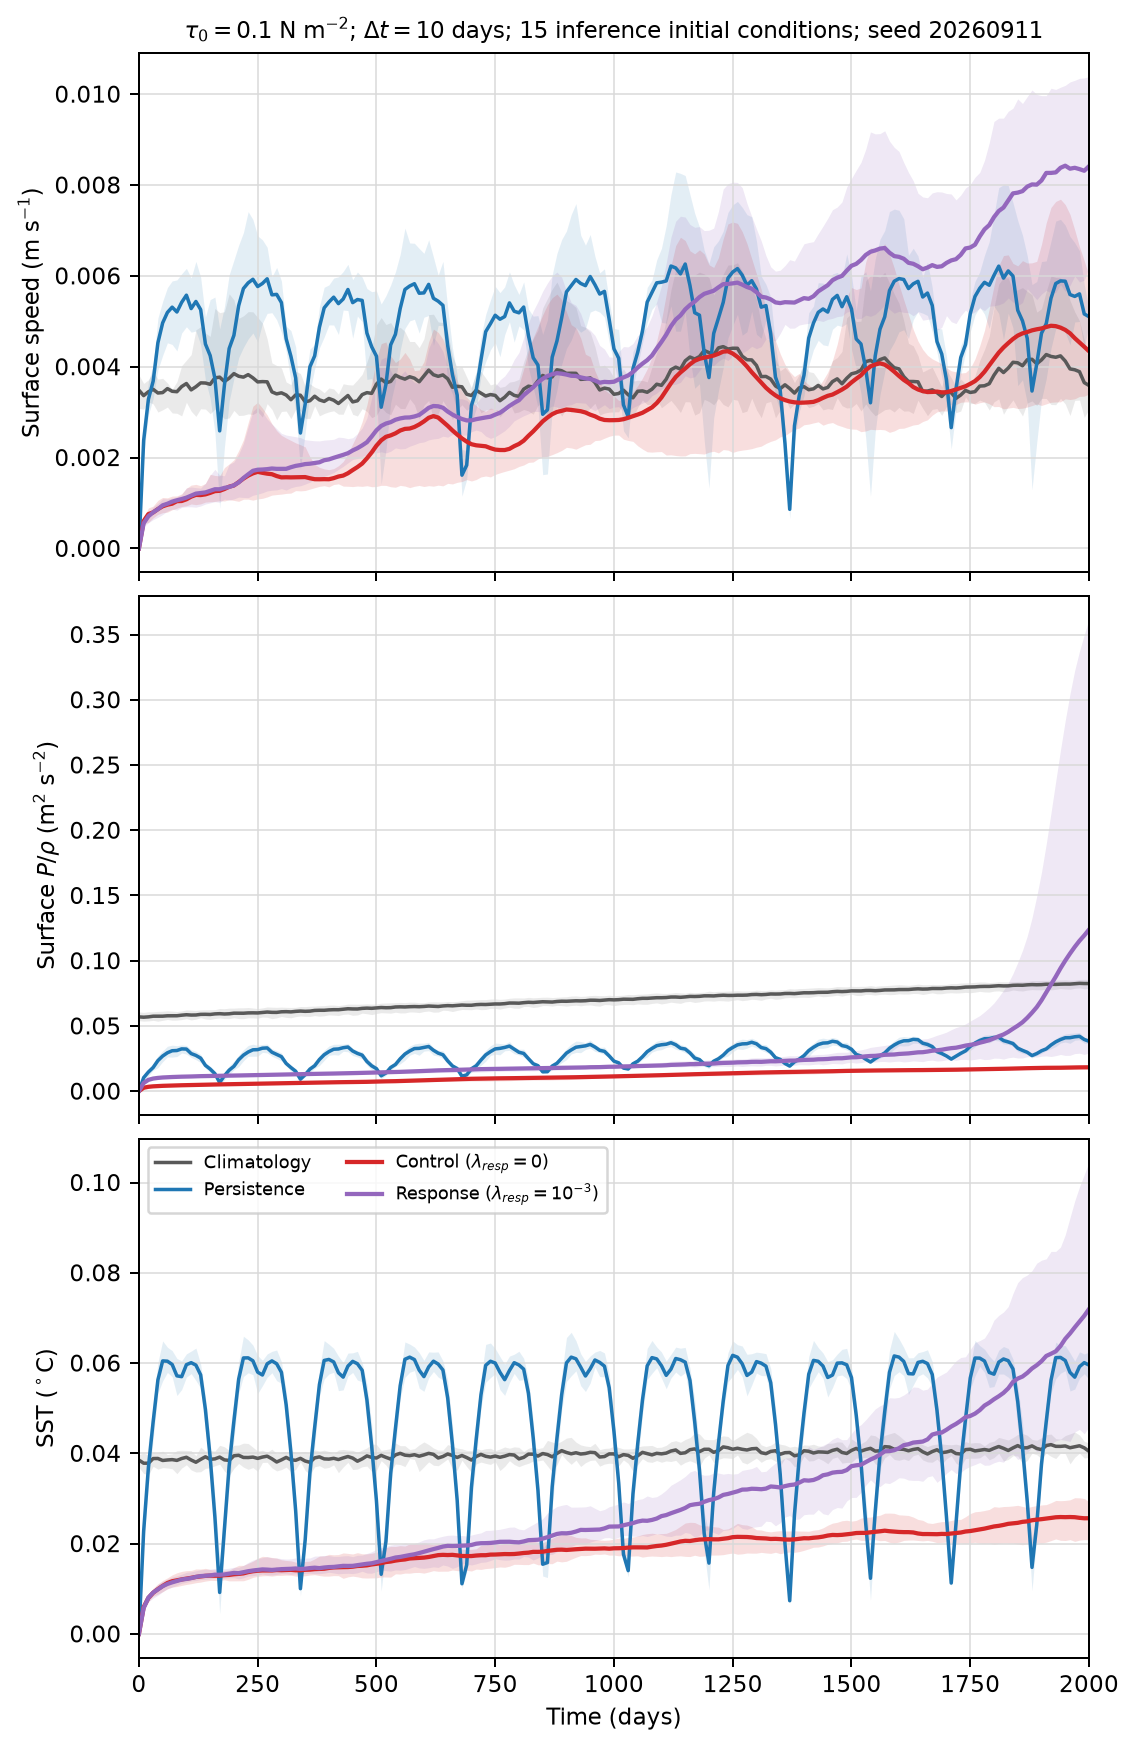
\includegraphics[width=0.72\textwidth]{figures/fwd_rmse_0_2000.png}
\caption{Pooled 15-member held-inference RMSE against \MITgcm{} truth,
$\Delta t=10$~d, days 0--2{,}000, S0, seed 20260911. Shading is the interdecile
range across members. The arms are indistinguishable to $\sim$day 800; the
response arm then crosses climatology in SST and surface pressure while the
control arm does not.}
\label{fig:fwd_rmse}
\end{figure}

\begin{figure}[htbp]
\centering
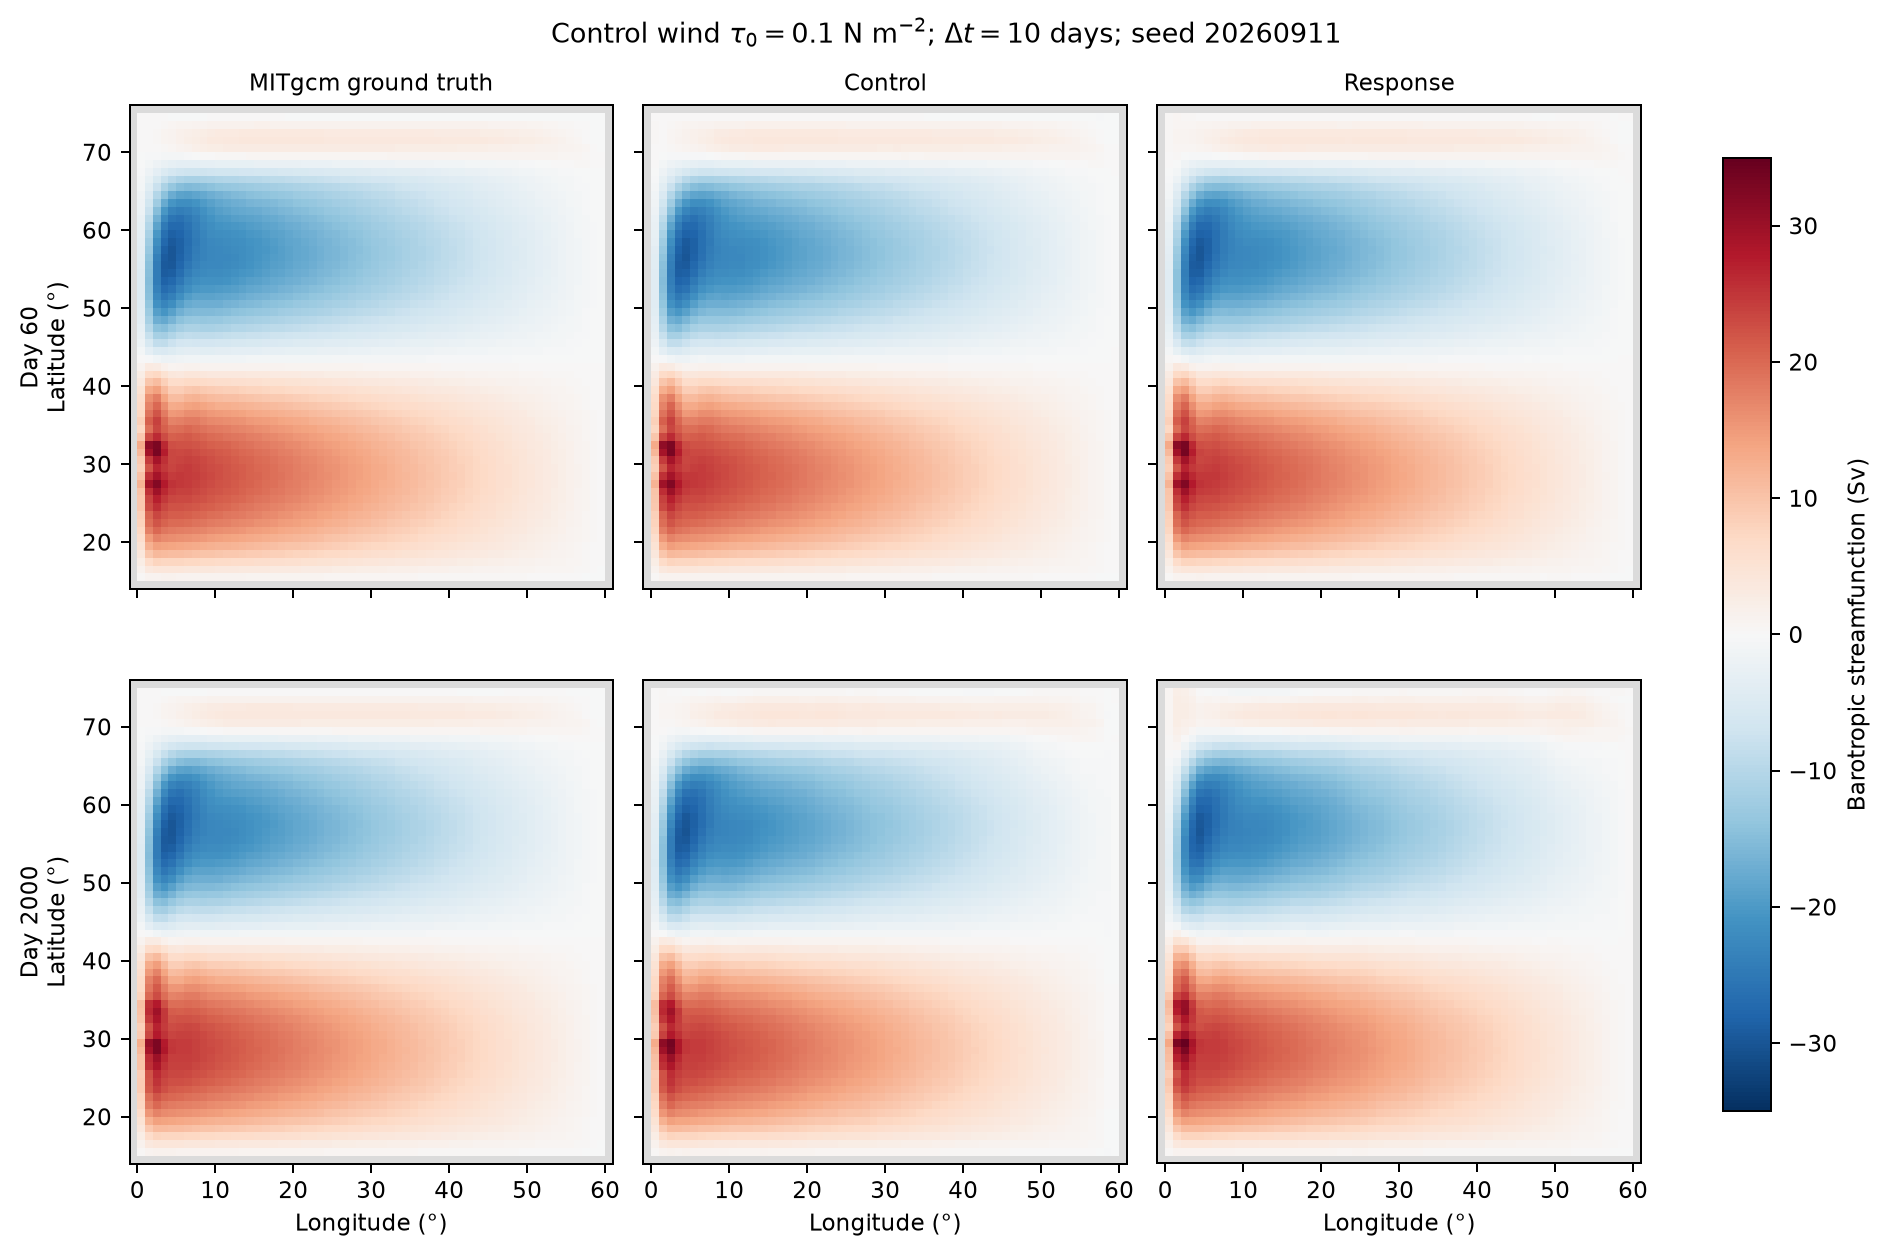
\includegraphics[width=\textwidth]{figures/fwd_stream.png}
\caption{Barotropic streamfunction $\psi$, day 60 (top) and day 2{,}000
(bottom): truth, control and response. Both arms reproduce the total gyre
circulation essentially indistinguishably from truth at both leads;
Figure~\ref{fig:fwd_stream_anom} removes the time-mean pedestal to show where
they actually differ.}
\label{fig:fwd_stream}
\end{figure}

\begin{figure}[htbp]
\centering
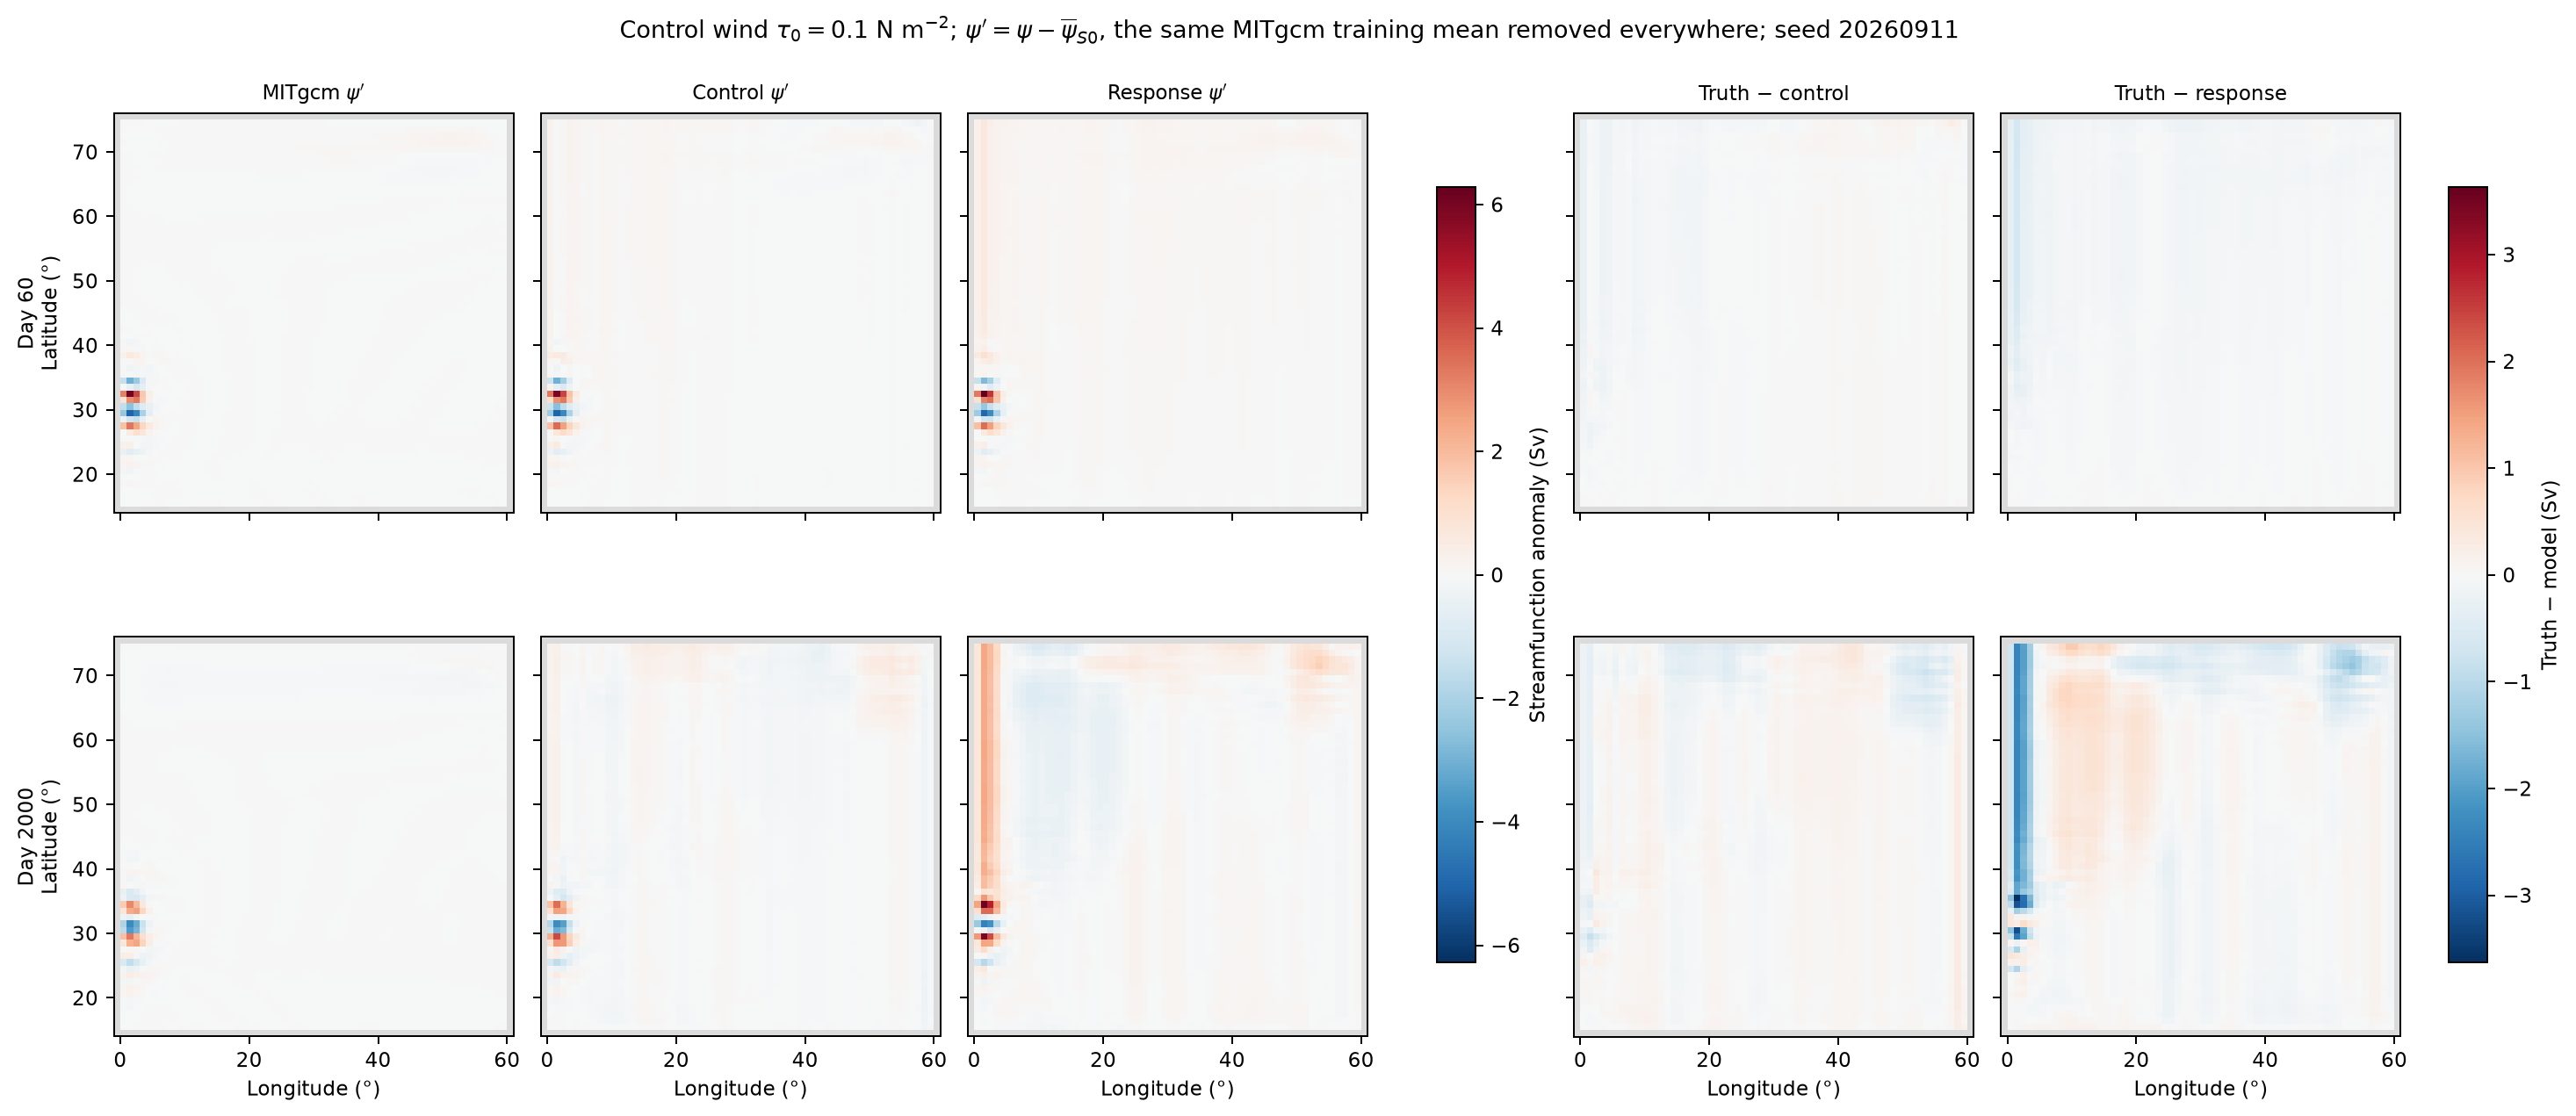
\includegraphics[width=\textwidth]{figures/fwd_stream_anomaly.png}
\caption{Barotropic streamfunction anomaly $\psi'$ about the \MITgcm{} S0
training mean, day 60 and day 2{,}000. Truth's day-2{,}000 anomaly is a compact
western-boundary dipole (0.74~Sv RMS); the control reproduces its amplitude
(0.81~Sv) and the response arm overshoots it by 2.2$\times$ (1.67~Sv) with a
spurious full-basin western band.}
\label{fig:fwd_stream_anom}
\end{figure}

\begin{figure}[htbp]
\centering
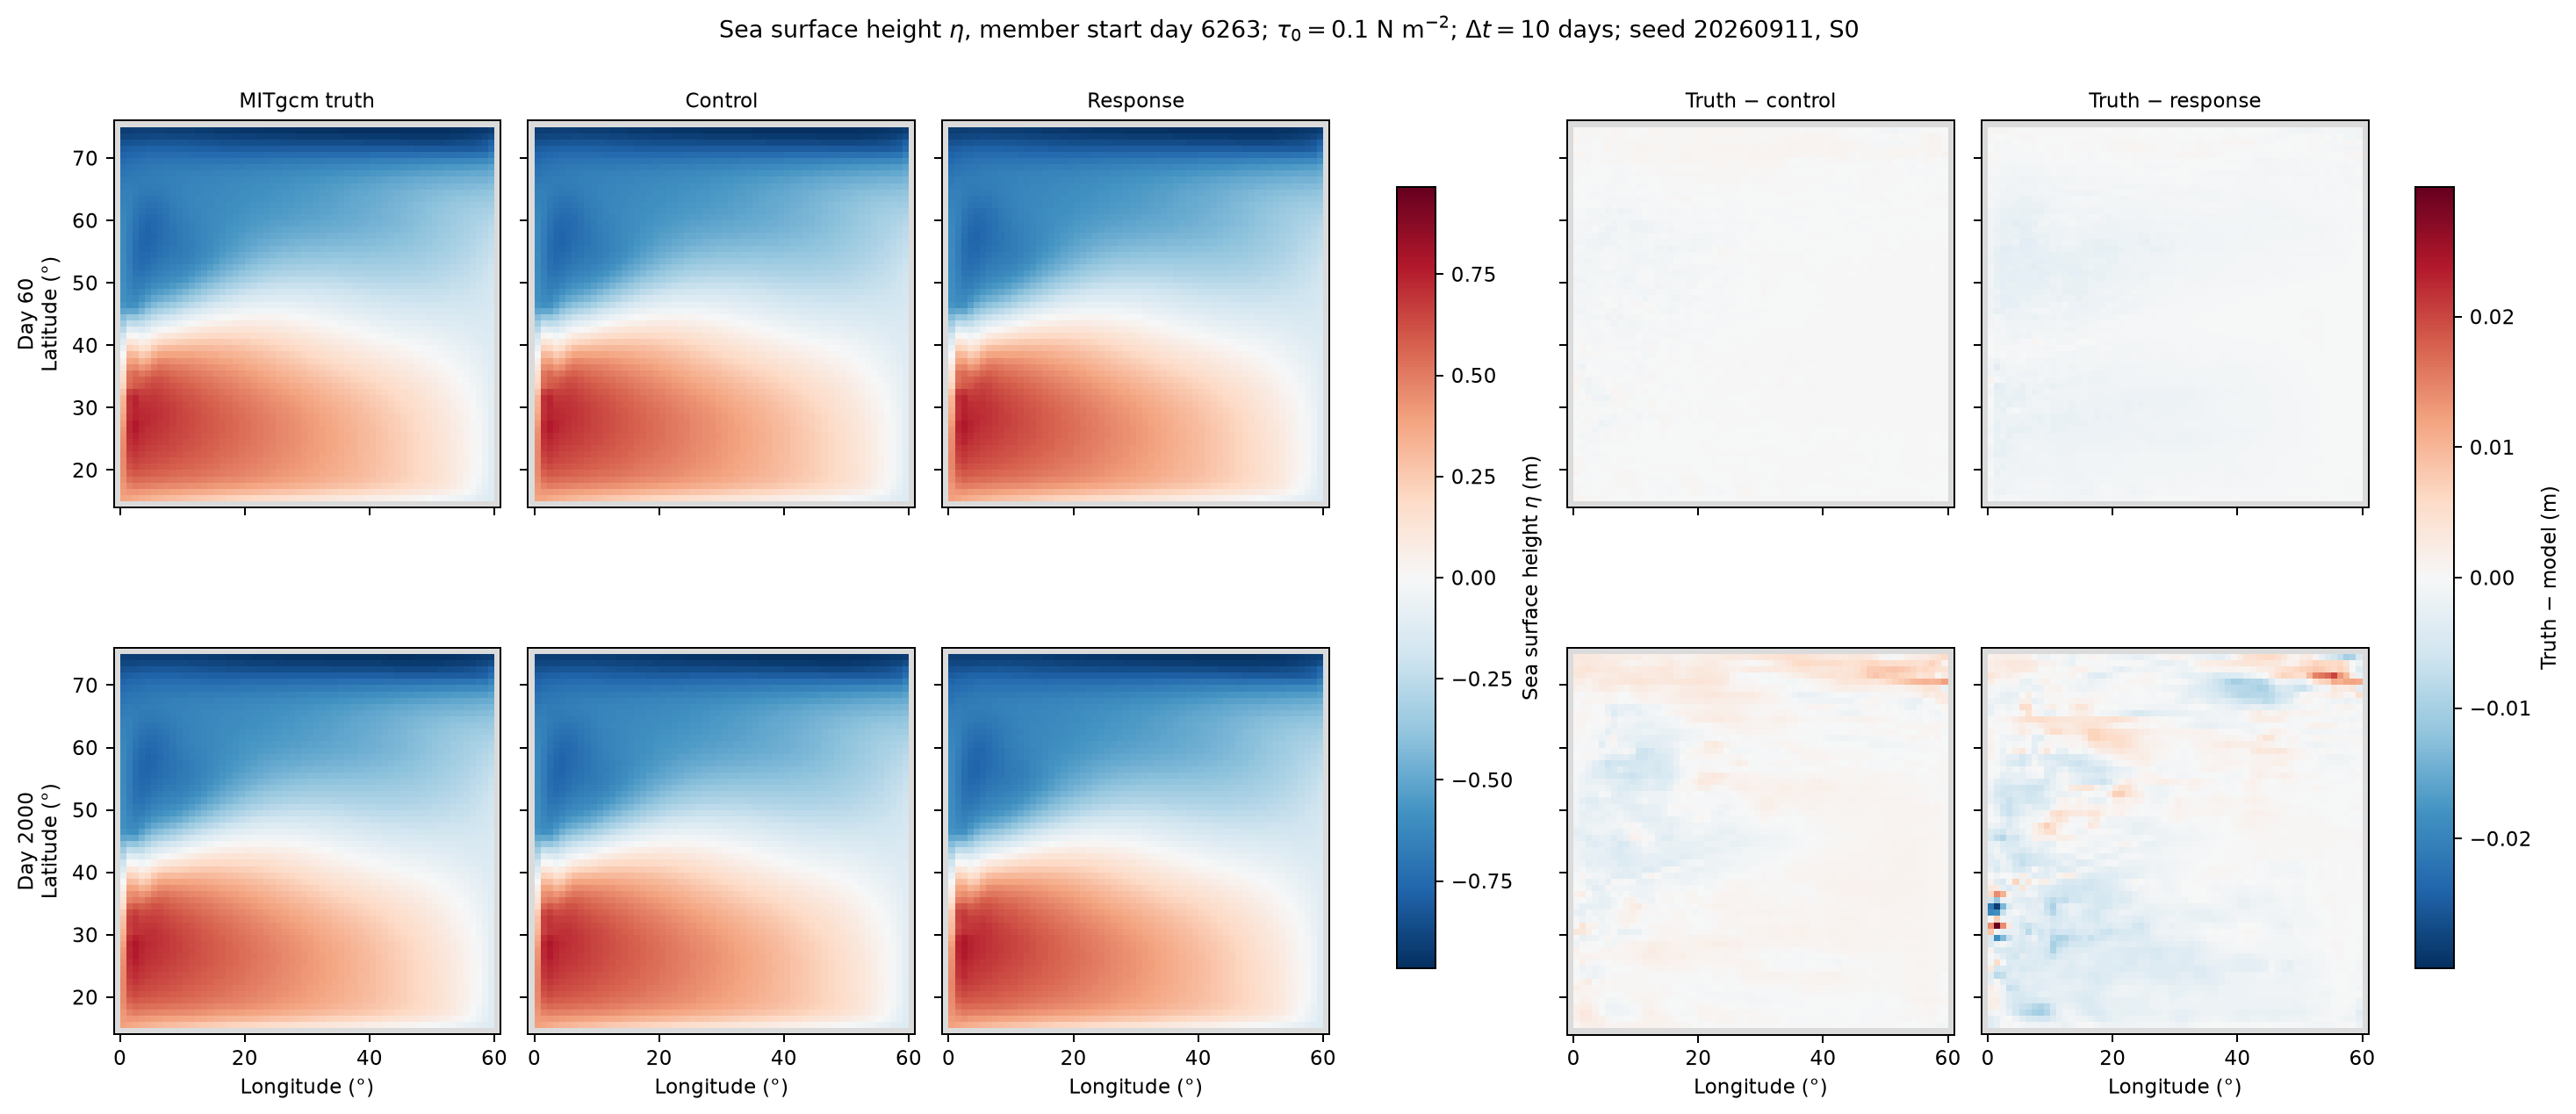
\includegraphics[width=\textwidth]{figures/fwd_ssh.png}
\caption{Sea surface height $\eta$, day 60 (top) and day 2{,}000 (bottom):
truth, control, response, and the two truth-minus-model differences on a shared
scale 40 times finer. Both arms reproduce the total field; the difference panels
carry the whole story, and even at day 2{,}000 they are two orders of magnitude
below the field.}
\label{fig:fwd_ssh}
\end{figure}

\begin{figure}[htbp]
\centering
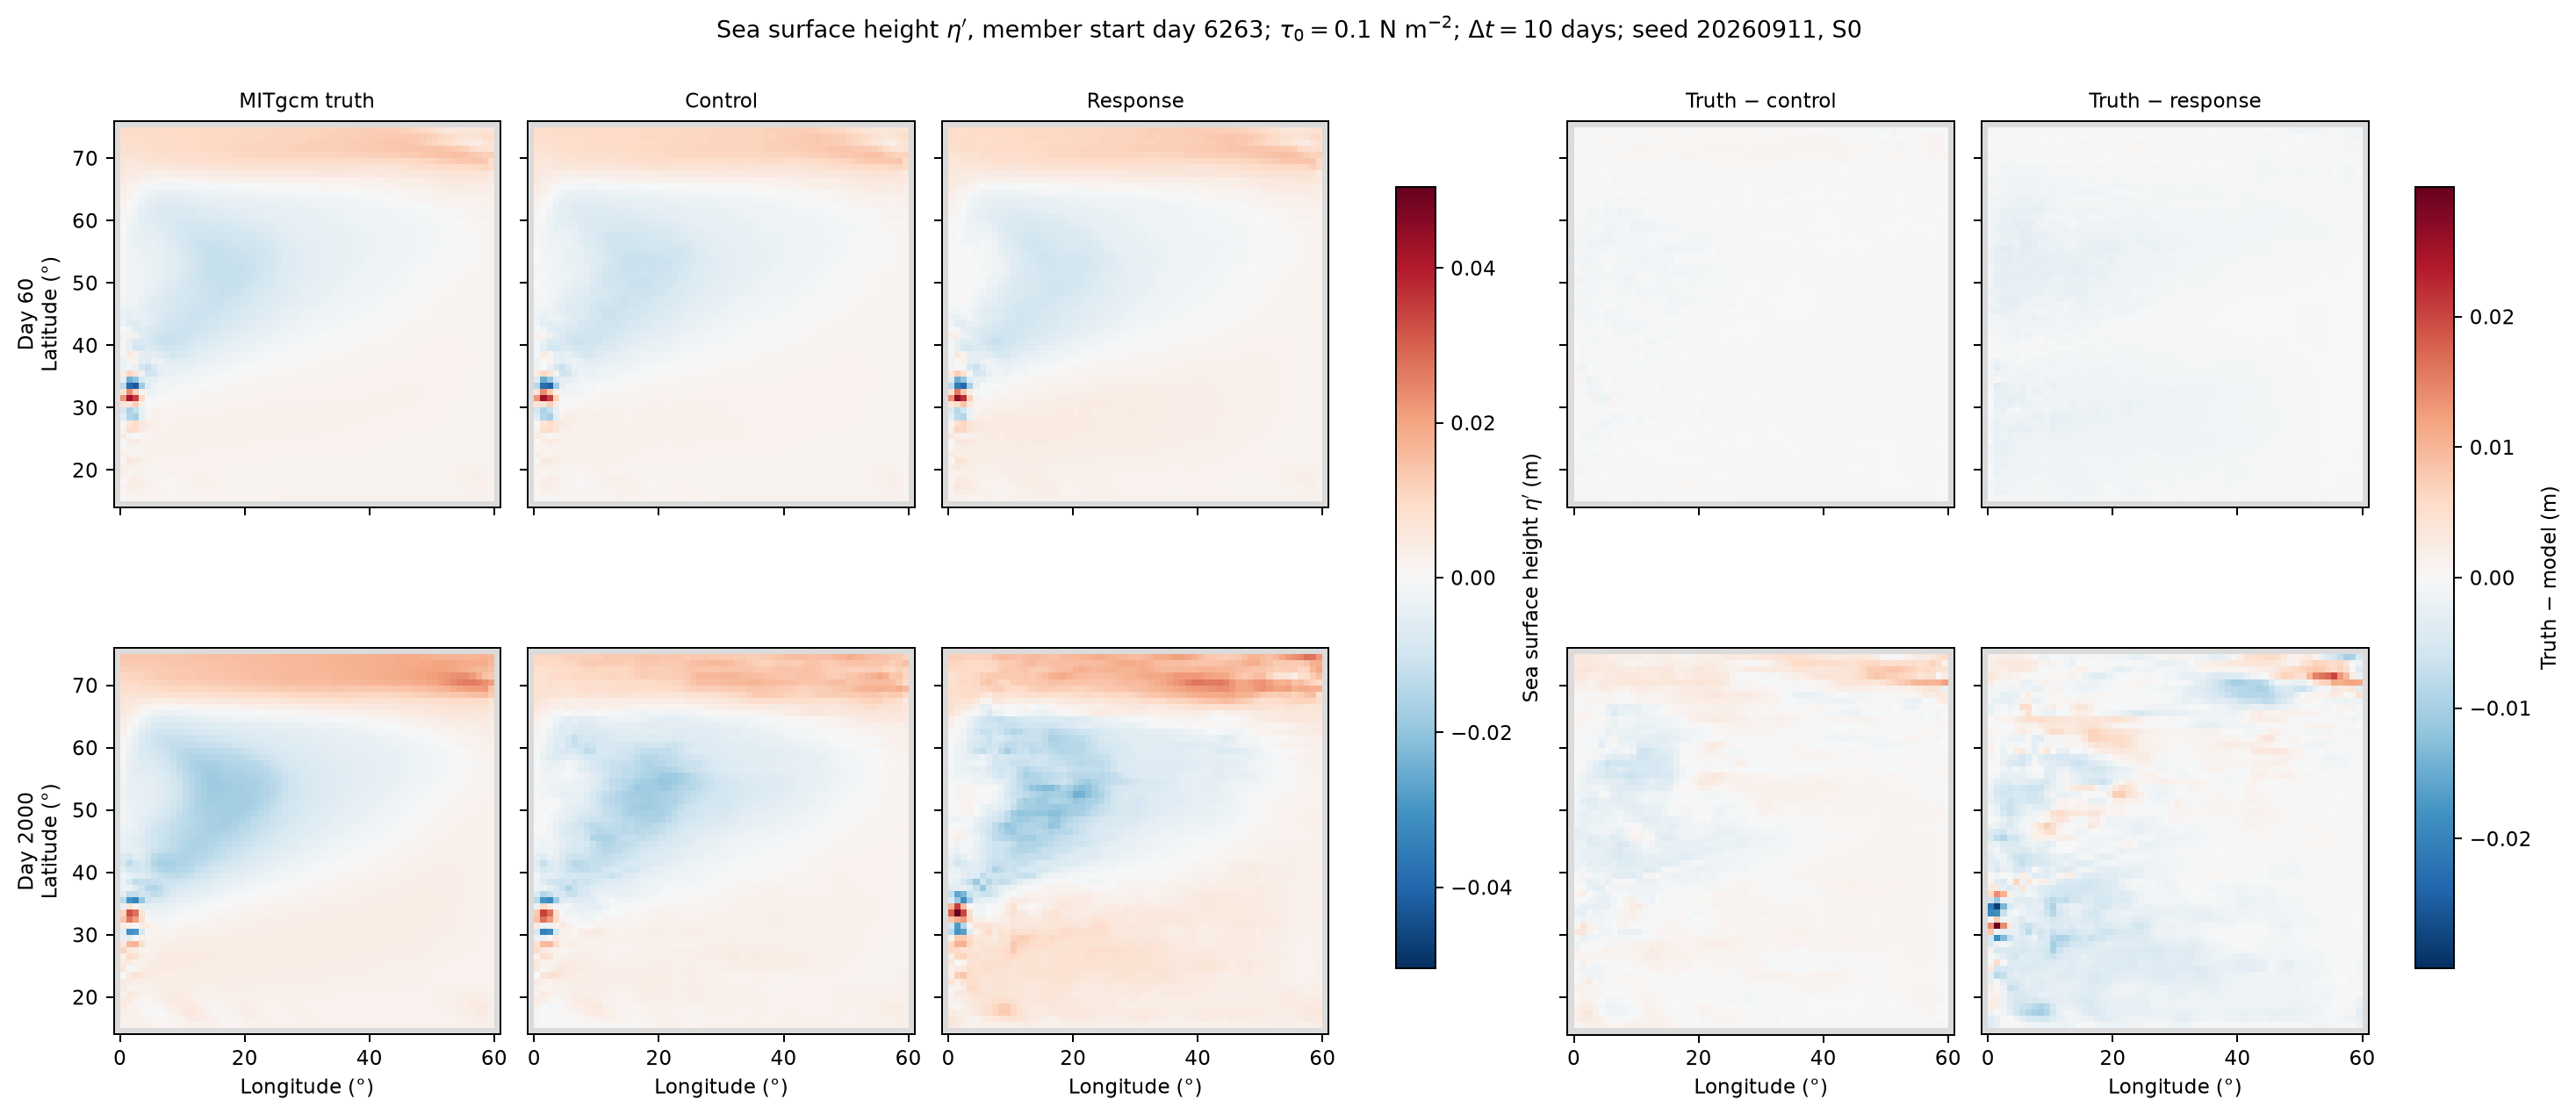
\includegraphics[width=\textwidth]{figures/fwd_ssh_anomaly.png}
\caption{Sea surface height anomaly $\eta'$, the same layout with the \MITgcm{}
S0 training-block time mean removed from truth and both models alike. At day
2{,}000 the response arm has grown a basin-scale dipole --- positive northern rim
and western boundary, negative interior --- that is absent from truth and from
the control.}
\label{fig:fwd_ssh_anom}
\end{figure}

\begin{figure}[htbp]
\centering
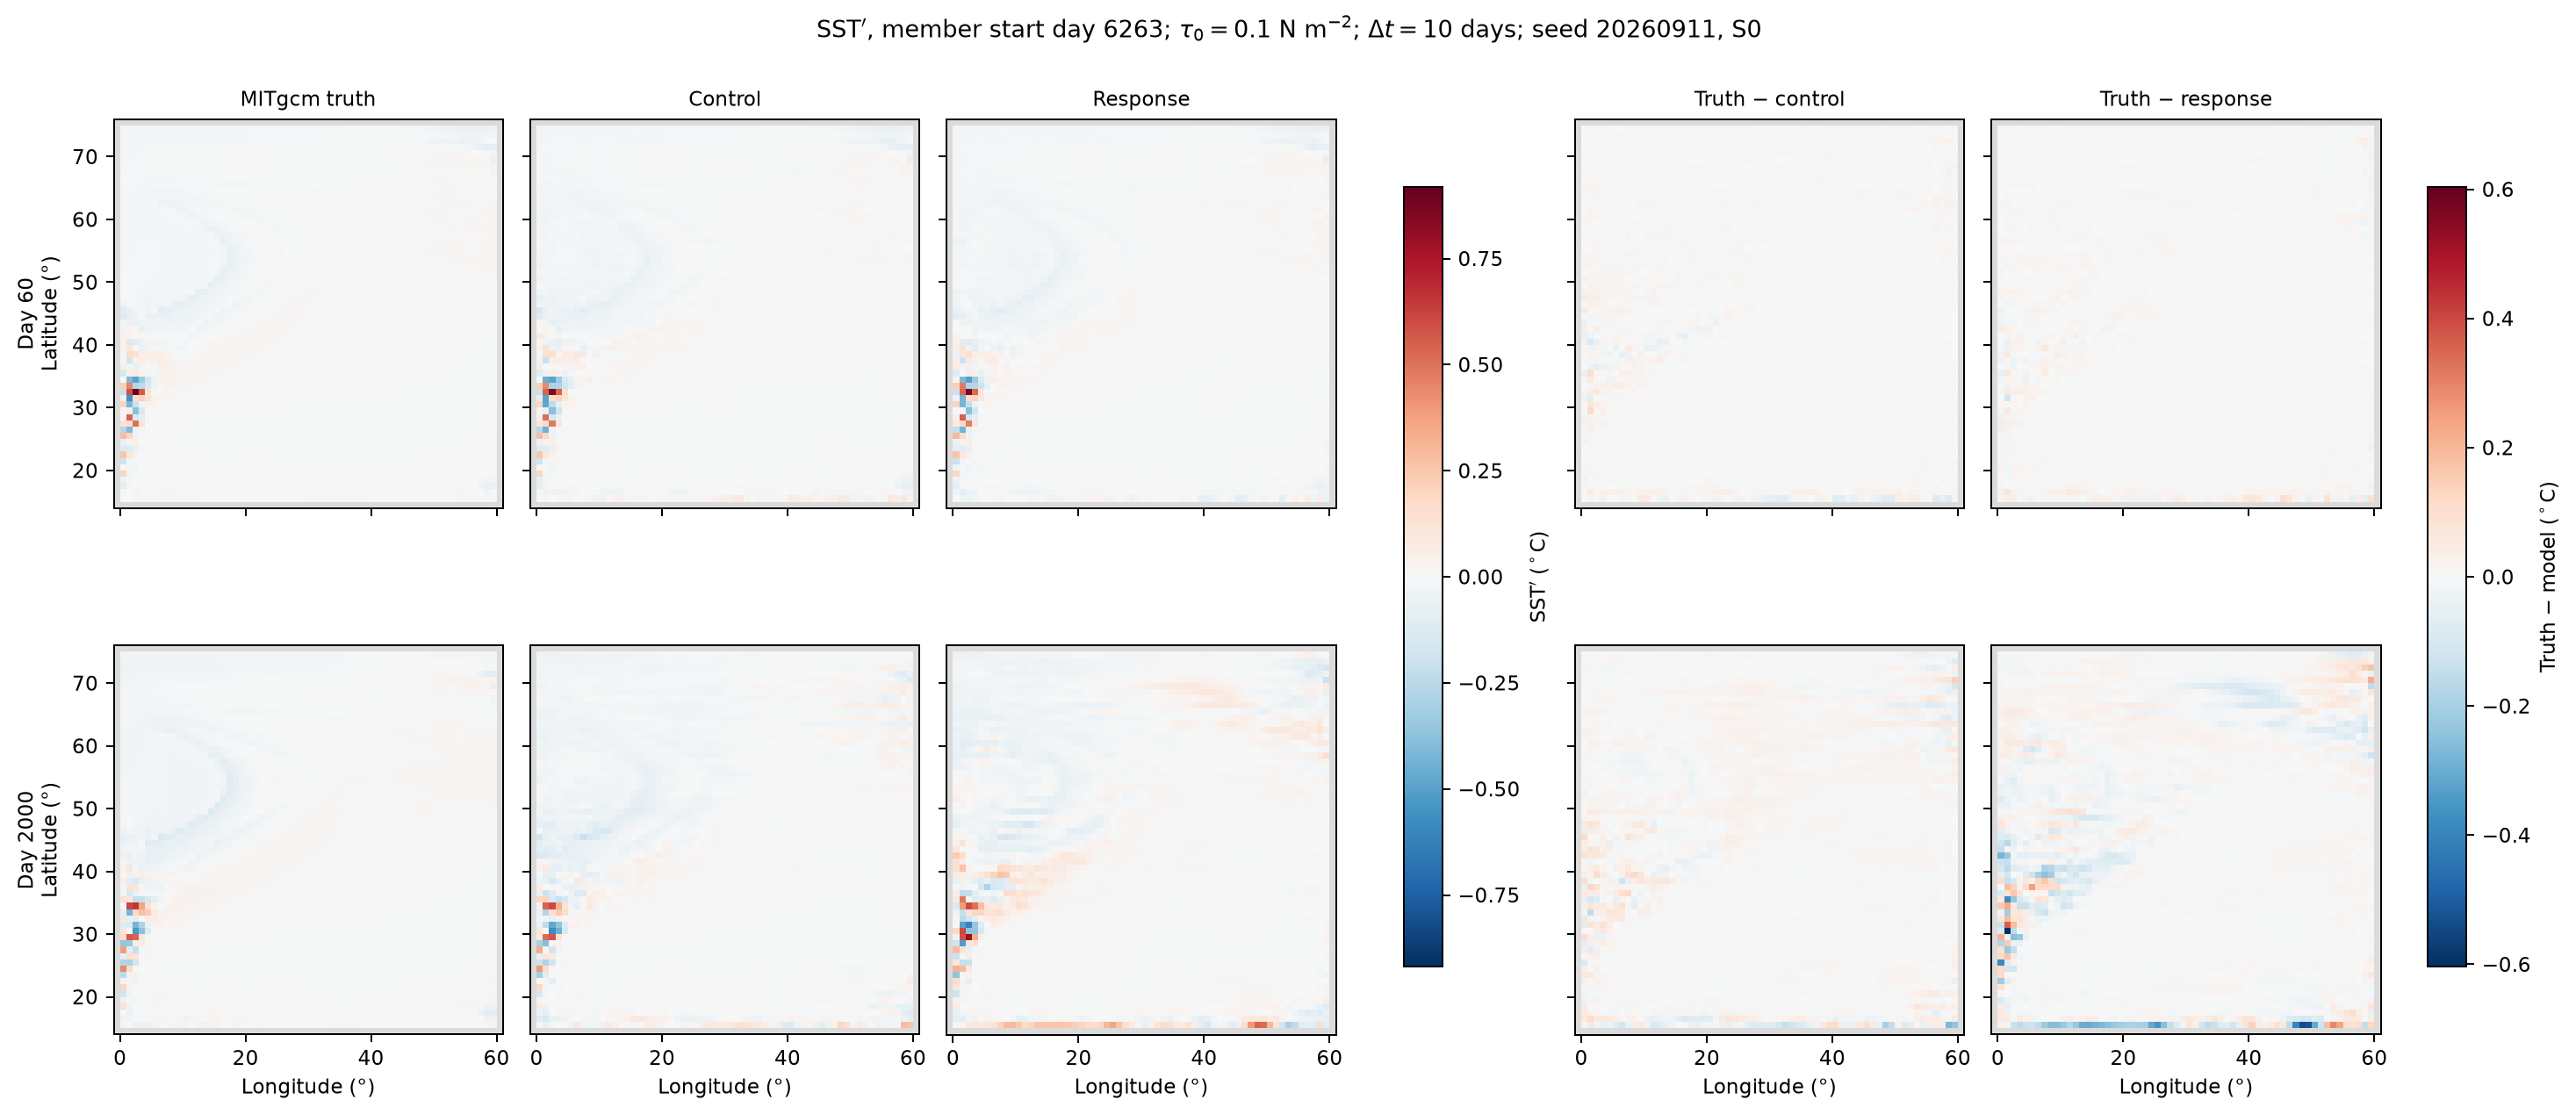
\includegraphics[width=\textwidth]{figures/fwd_sst_anomaly.png}
\caption{SST anomaly, day 60 and day 2{,}000. Both arms capture the
western-boundary front at day 60; by day 2{,}000 the response arm has added a
spurious warm plume along the jet axis and a warm band on the southern rim.}
\label{fig:fwd_sst_anom}
\end{figure}

\subsection{Control--response comparison, adjoint}
\label{sec:adjoint}

Every figure in this section uses the same layout: two rows, control
(\texttt{fno\_b\_seed\_\allowbreak 20260911}) above and response
(\texttt{fno\_c\_seed\_\allowbreak 20260911}) below, and three panels per row --- the
\MITgcm{}/TAF reference $S_T$, the emulator's $\Sforced$, and their difference.
Columns 1 and 2 share one colour scale so the amplitudes are directly comparable;
column 3 has its own. The open circle marks the target cell $p^\star$. The four
metrics of Eqs.~\eqref{eq:corr}--\eqref{eq:sign} are printed above each row.

Because the two rows plot the same physical reference, everything that differs
between them is attributable to the one training term.

\subsubsection{Mean conservation}
\label{sec:mean}

This is the one case whose exact answer is known analytically. With an implicit
free surface and \texttt{exactConserv}, the configuration conserves the
area-weighted basin-mean sea level exactly, so
$J_{\mathrm{mean}}(T)=\langle\eta(T)\rangle_A=\langle\eta(t_0)\rangle_A$ for
every $T$, and therefore
\begin{equation}
S^{\mathrm{mean}}_{T}[j,i] \;=\; \frac{\partial J_{\mathrm{mean}}}{\partial\eta(j,i,t_0)}
\;=\; w_{ji} \qquad\text{for all }T,
\label{eq:meanexact}
\end{equation}
independent of lead. The \MITgcm{}/TAF panel in Figures~\ref{fig:mean010}--\ref{fig:mean090}
is therefore literally the cell-area weight field: smooth, single-signed, and
$\propto\cos\phi$, hence largest in magnitude along the southern boundary where
cells are widest ($\max|S|=3.96\times10^{-4}$, exactly $1.43\times$ the uniform
value $1/3600$, as $\cos(15.5^\circ)$ over the domain-mean cosine requires). It
is identical at every lead, verified to $3.57\times10^{-8}$ over 91 daily dumps.
The correct amplitude ratio is exactly $\alpha=1$ at every lead, and any
departure is unambiguously emulator error.

\begin{table}[H]
\centering
\small
\begin{tabular}{lrrrrrr}
\toprule
& \multicolumn{3}{c}{Control} & \multicolumn{3}{c}{Response} \\
\cmidrule(lr){2-4}\cmidrule(lr){5-7}
Lead (d) & $\rho$ & $\varepsilon_2$ & $\alpha$ & $\rho$ & $\varepsilon_2$ & $\alpha$ \\
\midrule
10 & $+0.907$ & 0.626 & 0.380 & $+0.927$ & 0.632 & 0.373 \\
30 & $+0.625$ & 0.949 & 0.055 & $+0.698$ & 0.950 & 0.053 \\
90 & $+0.012$ & 1.002 & 0.007 & $-0.031$ & 1.000 & 0.003 \\
\bottomrule
\end{tabular}
\caption{Basin-mean conservation. The exact answer is $\rho=1$,
$\varepsilon_2=0$, $\alpha=1$ at every lead. Both arms damp the conserved mode
at a near-constant factor per ten-day call.}
\label{tab:mean}
\end{table}

Both models fail this test, and they fail it in a specific, interpretable way.
After a single ten-day call the emulator has retained only 38\% of the conserved
mode ($\alpha=0.380$ control, $0.373$ response) --- but with pattern correlation
0.91--0.93, meaning it has the shape of the weight field almost right and simply
scaled it down. The decay is close to geometric in the number of calls: three
calls give $0.380^{3}=0.0549$ against a measured 0.055, and $0.373^{3}=0.0519$
against a measured 0.053. In other words, both emulators apply an approximately
constant damping factor of $\approx0.38$ per call to the one mode the ocean model
conserves exactly. By lead 90 the mode is gone (amplitude ratios $0.007$ and
$0.003$; the residual decays more slowly than the pure geometric law would
predict, so a faint remnant survives), the pattern correlation has collapsed to
zero, and $\varepsilon_2\to1.00$ --- the value $\varepsilon_2$ takes when the
emulator map is simply absent, since $\|S^{F}-S^{M}\|\to\|S^{M}\|$.

This is a qualitatively different failure from every other case in this section.
Everywhere else the emulator is \emph{too} sensitive by factors of 5 to 47; here
it is not sensitive enough by a factor of 3 to 300. A neutral mode --- one whose
true amplification factor is exactly 1 --- is precisely what an
autoregressive-stability regularizer suppresses, and the per-mode spectral
normalization caps every channel-mixing matrix at unit norm, which cannot amplify
but readily damps. Improved mean-mode preservation was a named secondary endpoint
of the study; the response term moves it slightly in the wrong direction.

\begin{figure}[htbp]
\centering
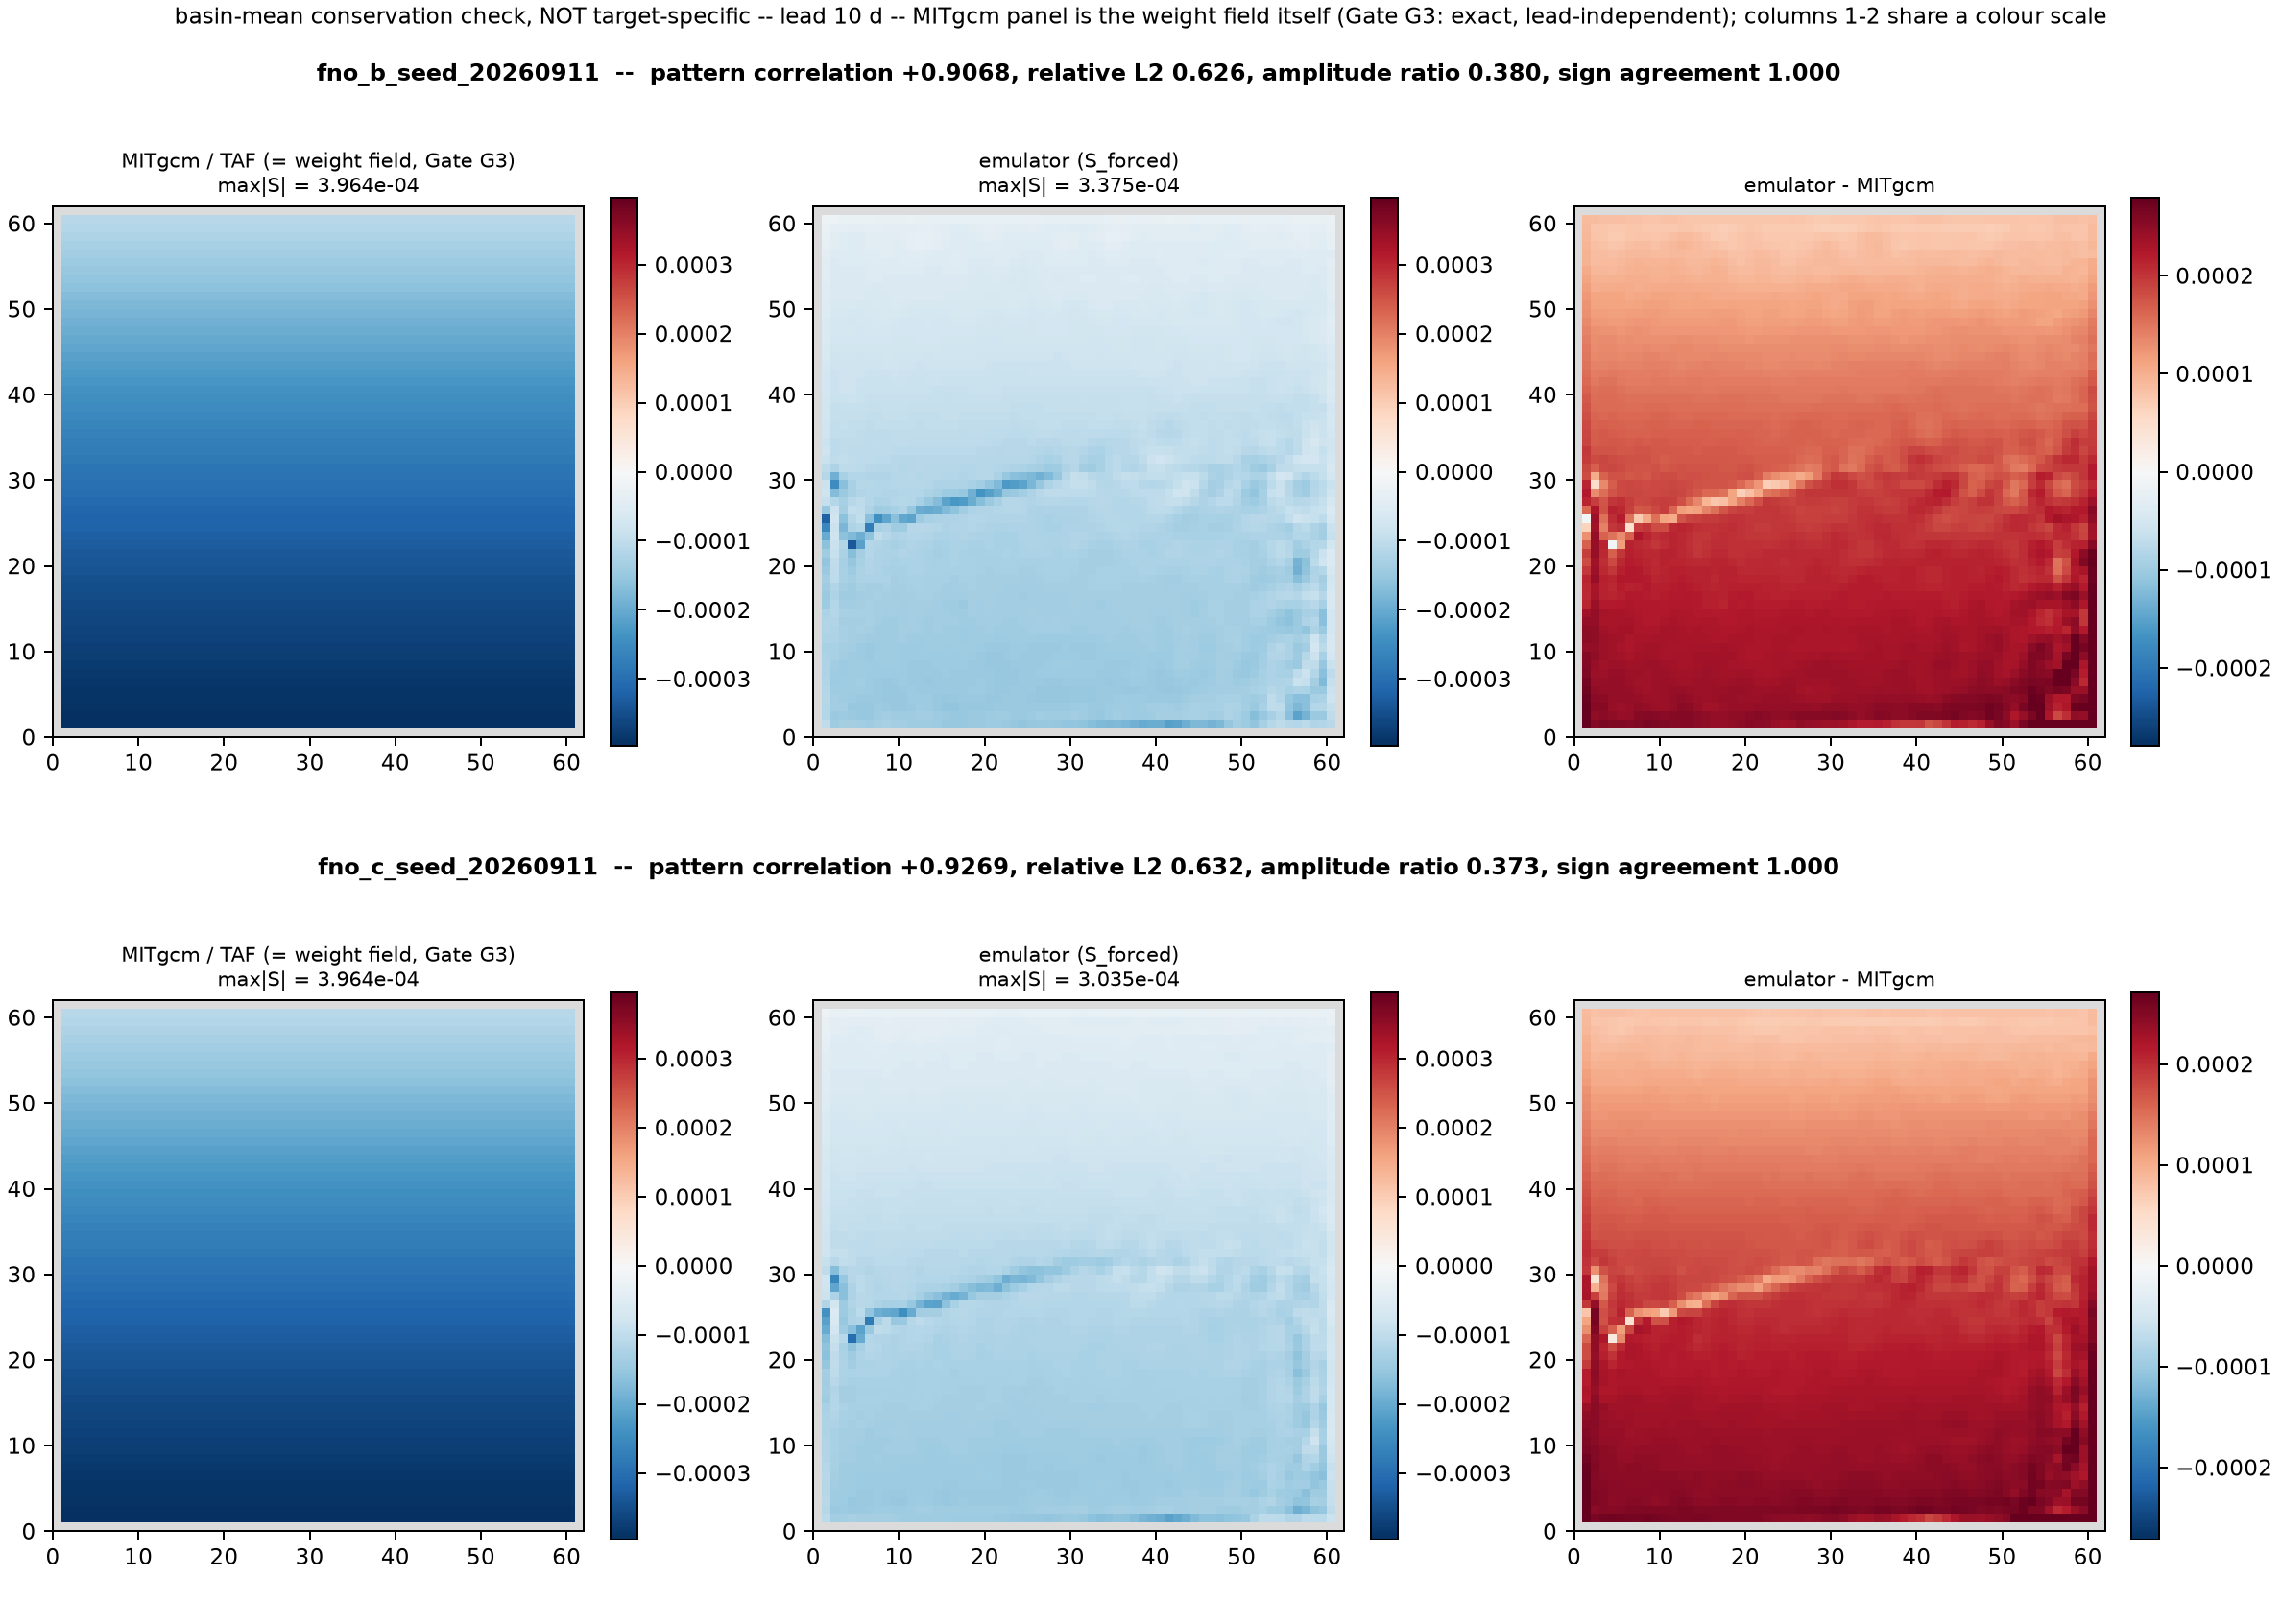
\includegraphics[width=\textwidth]{figures/adj_mean_010.png}
\caption{Basin-mean conservation, lead 10~d. The \MITgcm{} panel is the exact
area-weight field, Eq.~\eqref{eq:meanexact}. Both emulators recover its shape
($\rho\approx0.91$--0.93) at 38\% of its amplitude; the visible fine structure
along the jet axis in the emulator panels is spurious.}
\label{fig:mean010}
\end{figure}

\begin{figure}[htbp]
\centering
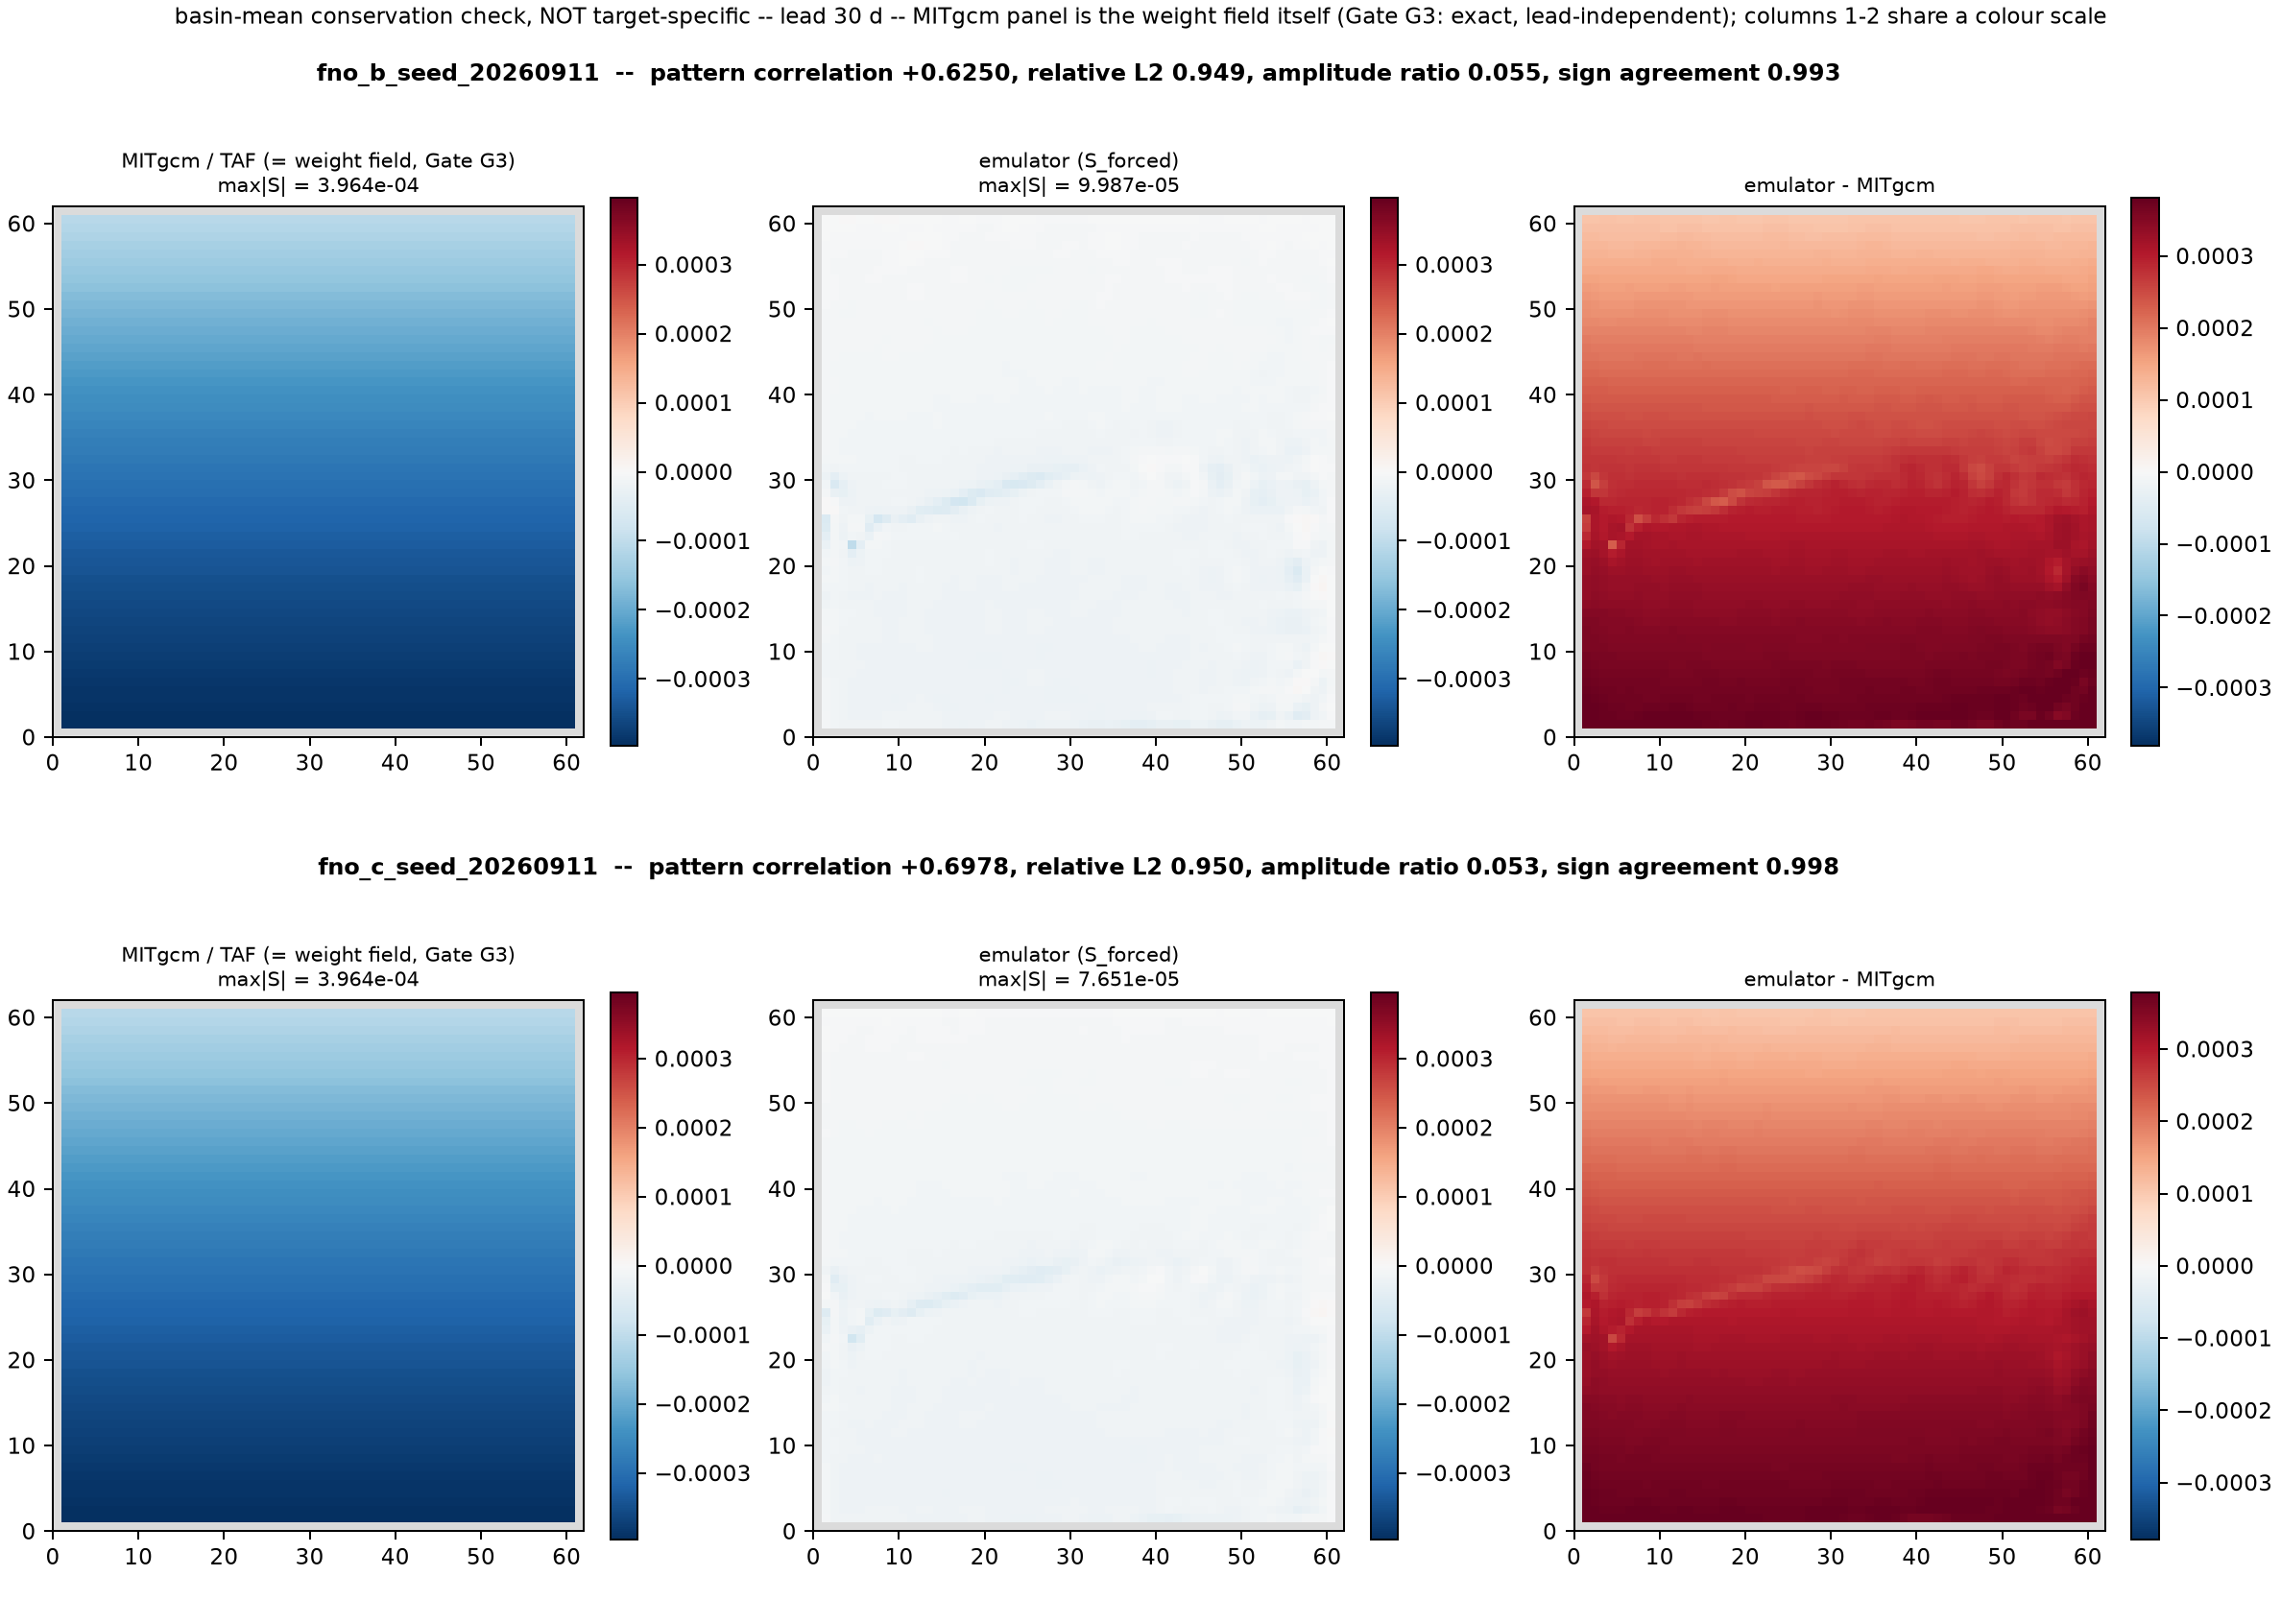
\includegraphics[width=\textwidth]{figures/adj_mean_030.png}
\caption{Basin-mean conservation, lead 30~d (three calls). The reference is
unchanged; the emulator amplitude has fallen to $\approx0.38^{3}\approx0.055$ of
truth for both arms, and the pattern correlation has already dropped to
0.63--0.70.}
\label{fig:mean030}
\end{figure}

\begin{figure}[htbp]
\centering
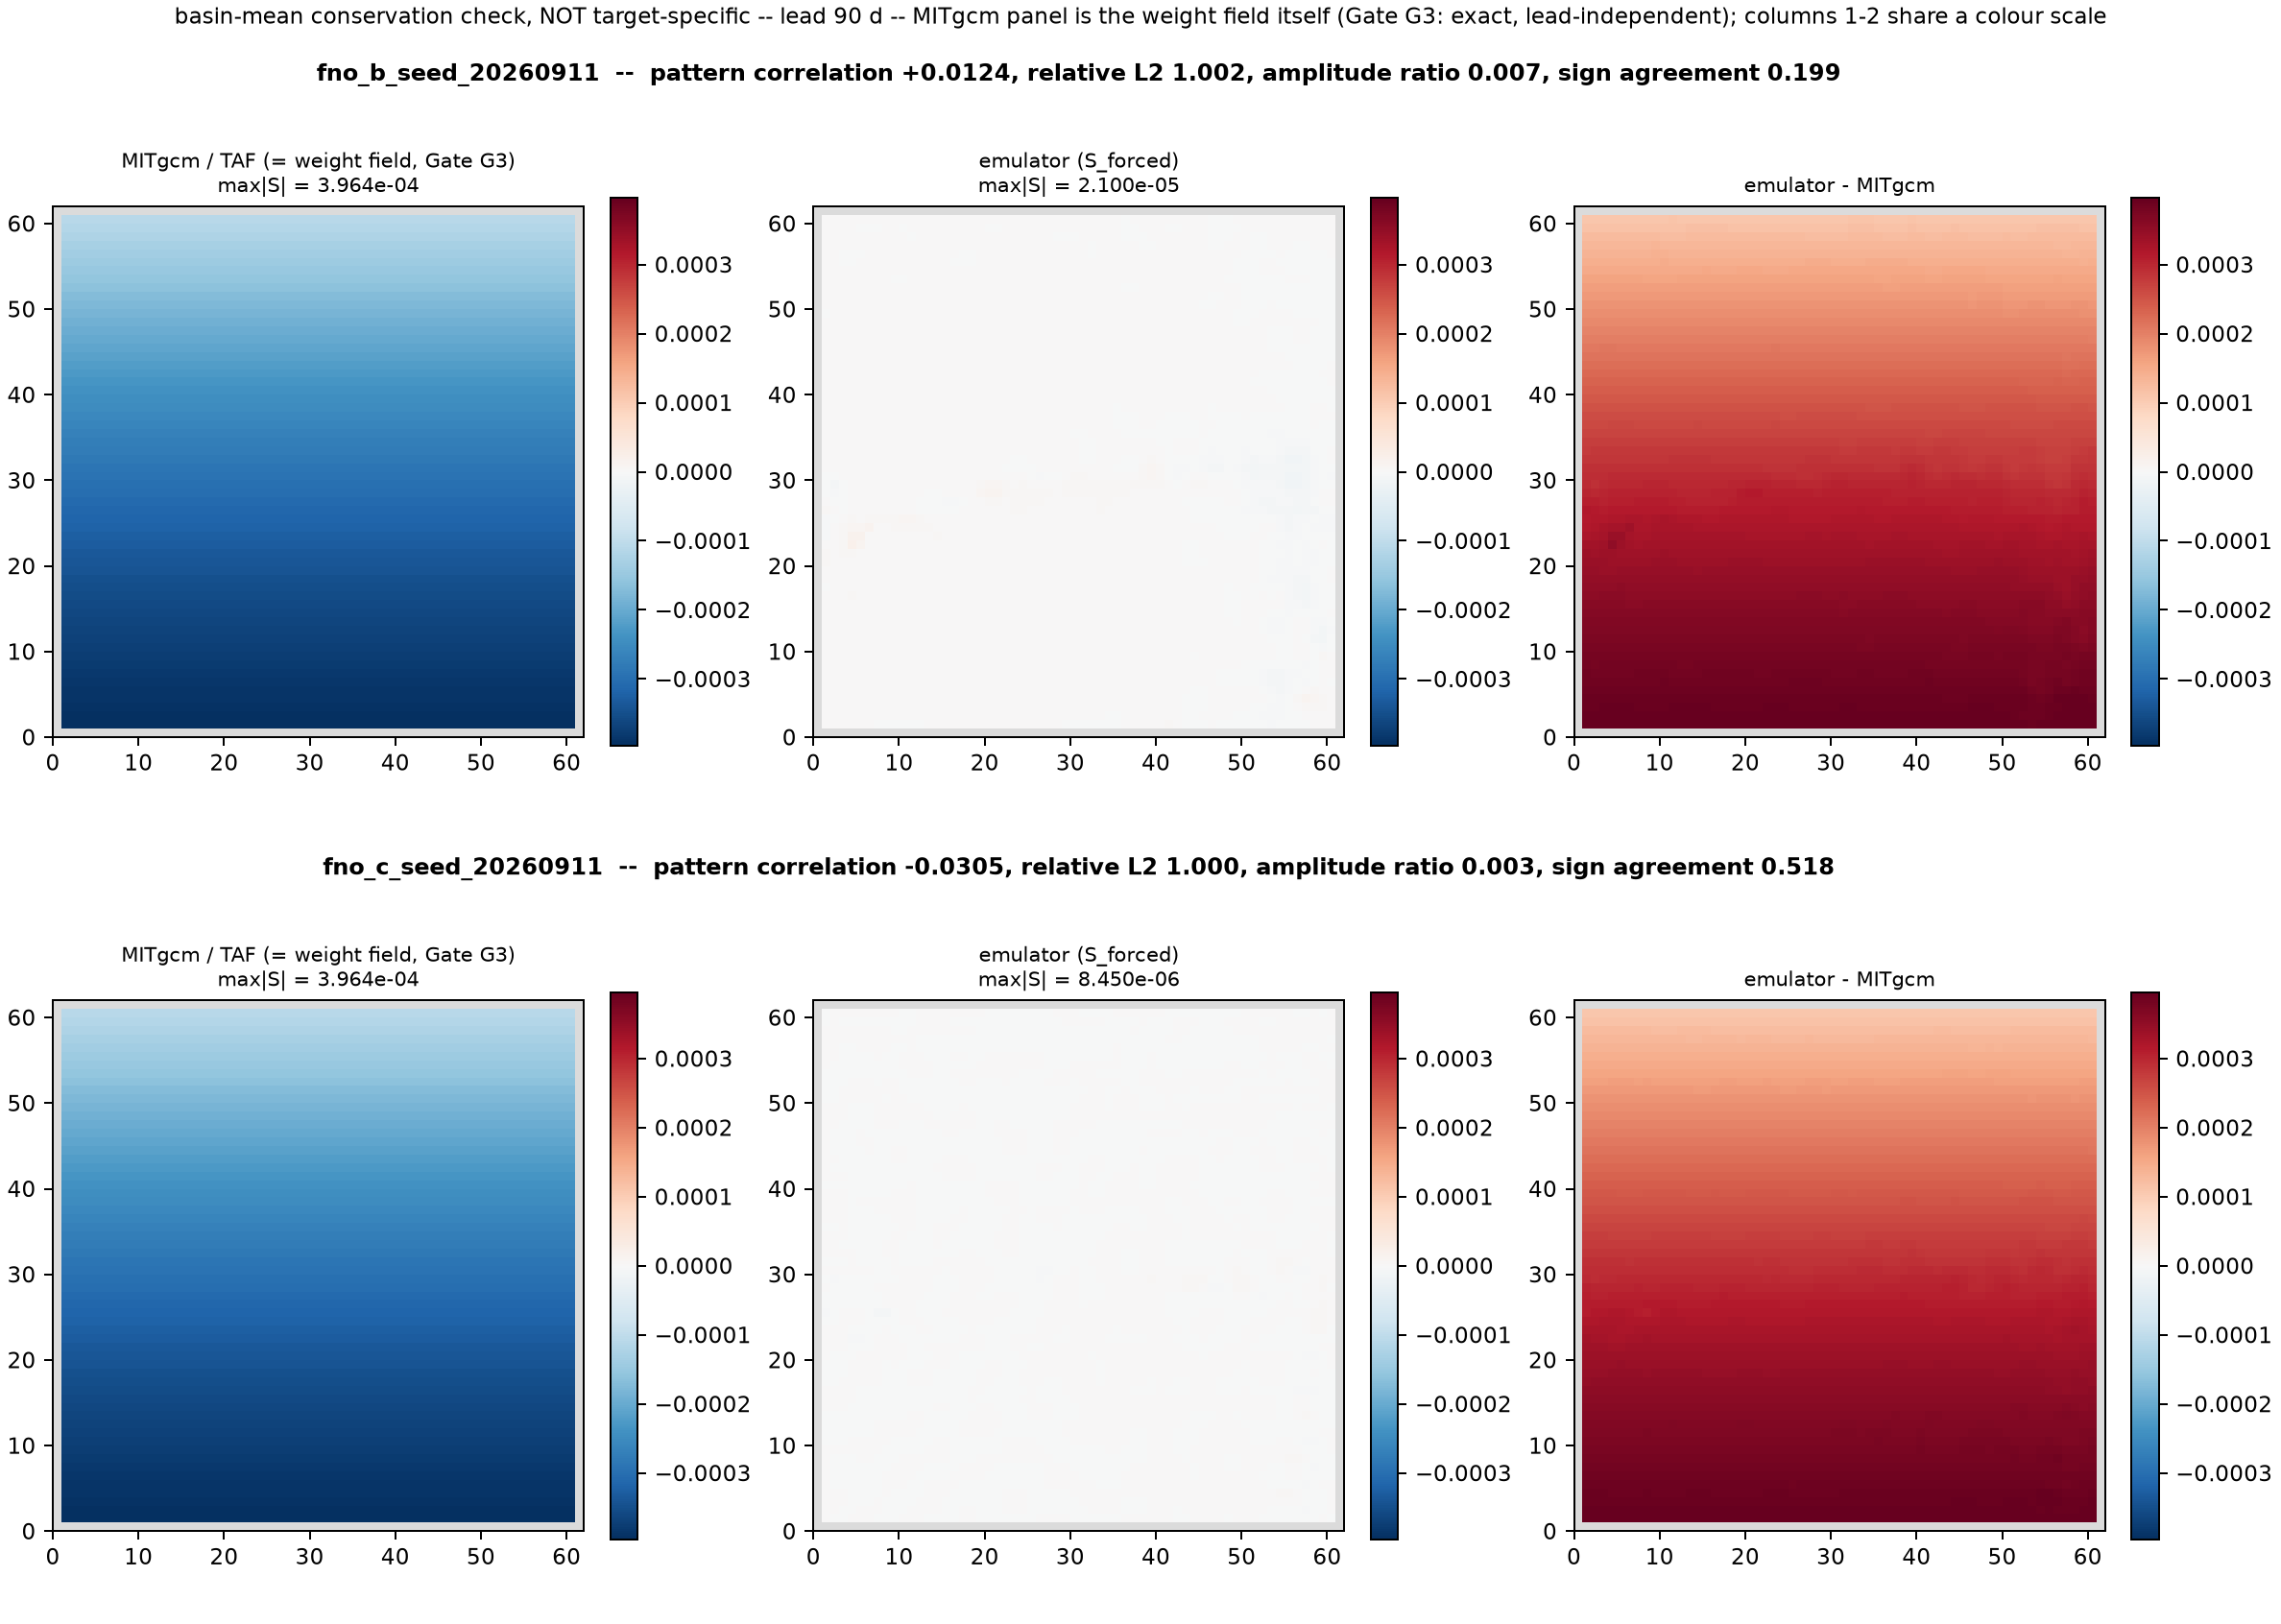
\includegraphics[width=\textwidth]{figures/adj_mean_090.png}
\caption{Basin-mean conservation, lead 90~d. The emulator panels are
essentially blank on the shared scale: the conserved mode has been damped out of
existence, and the difference panel is the reference field with its sign
flipped.}
\label{fig:mean090}
\end{figure}

\subsubsection{Interior target}
\label{sec:interior}

The interior target sits at $(i,j)=(31,17)$, mid-basin, roughly half a domain
width from either wall.

\begin{table}[H]
\centering
\small
\begin{tabular}{llrrrrrr}
\toprule
& & \multicolumn{3}{c}{Control} & \multicolumn{3}{c}{Response} \\
\cmidrule(lr){3-5}\cmidrule(lr){6-8}
Objective & Lead (d) & $\rho$ & $\varepsilon_2$ & $\alpha$ & $\rho$ & $\varepsilon_2$ & $\alpha$ \\
\midrule
$J_{\mathrm{raw}}$  & 10 & $+0.125$ & 8.330 & 8.363 & $+0.125$ & \textbf{8.209} & 8.243 \\
$J_{\mathrm{raw}}$  & 30 & $+0.078$ & 1.163 & 0.696 & $+0.082$ & \textbf{1.152} & 0.682 \\
$J_{\mathrm{raw}}$  & 90 & $-0.121$ & 1.016 & 0.108 & $-0.010$ & \textbf{1.001} & 0.047 \\
$J_{\mathrm{anom}}$ & 10 & $+0.120$ & 20.285 & 20.381 & $+0.121$ & \textbf{19.991} & 20.086 \\
$J_{\mathrm{anom}}$ & 30 & $+0.049$ & 2.115 & 1.913 & $+0.056$ & \textbf{2.074} & 1.874 \\
$J_{\mathrm{anom}}$ & 90 & $-0.152$ & 1.136 & 0.409 & $-0.001$ & \textbf{1.016} & 0.177 \\
\bottomrule
\end{tabular}
\caption{Interior target $(31,17)$. Bold marks the lower relative $L_2$ of the
two arms; the response arm is lower in all six cells.}
\label{tab:interior}
\end{table}

\paragraph{Raw SSH (Figures~\ref{fig:int_raw010}--\ref{fig:int_raw090})} The
reference maps show what fast barotropic adjustment looks like in an adjoint. At
lead 10 the true sensitivity is already basin-wide: a broad positive field
everywhere --- the conserved-mean pedestal of Eq.~\eqref{eq:meanexact}, which
$J_{\mathrm{raw}}$ does not remove --- with a strong positive lobe fanning
east and north-east from the target and a weak negative notch just upstream of
it. Ten days is long enough for a sea-level perturbation anywhere in the basin to
have influenced the target. The emulator's map is nothing like this. It is a
near-delta at the target cell itself ($\max|S|=1.12\times10^{-1}$ against
$9.6\times10^{-4}$ for truth, a factor of 116 at the peak) surrounded by
fine-grained, sign-alternating speckle concentrated along the jet axis at
$j\approx30$ and against the eastern wall. The emulator's ten-day Jacobian is,
in effect, almost the identity plus grid-scale noise: it has learned that
sea level ten days from now looks like sea level today at the same place, which
is an excellent \emph{forecast} and a completely wrong \emph{derivative}. The
resulting amplitude ratio is 8.4.

By lead 30 the two amplitudes have crossed: the true sensitivity has continued to
spread and grow while the emulator's has decayed, giving $\alpha=0.70$ and
$\varepsilon_2=1.16$. By lead 90 the reference is a smooth, everywhere-positive
field with a broad maximum draped over the target and the jet, while the emulator
retains only a small dipole at the target and traces along the jet, at 11\%
(control) and 4.7\% (response) of the true amplitude. The pattern correlation is
now slightly \emph{negative}. Note that the two arms differ visibly here: the
control keeps a stronger localized dipole ($\max|S|=6.4\times10^{-4}$) than the
response ($1.2\times10^{-4}$), and the response's lower $\varepsilon_2$ at this
lead comes from being closer to zero, not from being closer to truth.

\paragraph{SSH anomaly (Figures~\ref{fig:int_anom010}--\ref{fig:int_anom090})}
Removing the basin mean removes the pedestal and leaves the dynamically
interesting part: at lead 90 the true map is a clean two-lobed structure --- a
broad positive region enveloping the target and extending south-east, a negative
region hugging the western boundary --- which is the imprint of westward Rossby
propagation carrying information from the east back toward the target. The
emulator maps show no trace of it: the control has a small target-centred dipole
plus jet-axis speckle, the response is nearly featureless. Because the reference
norm is smaller once the pedestal is gone, the lead-10 amplitude ratios are
correspondingly larger (20.4 and 20.1). The response arm's improvement is
consistent but small: relative $L_2$ falls by 1.4\%, 1.9\% and 10.6\% at leads
10, 30 and 90.

\begin{figure}[htbp]
\centering
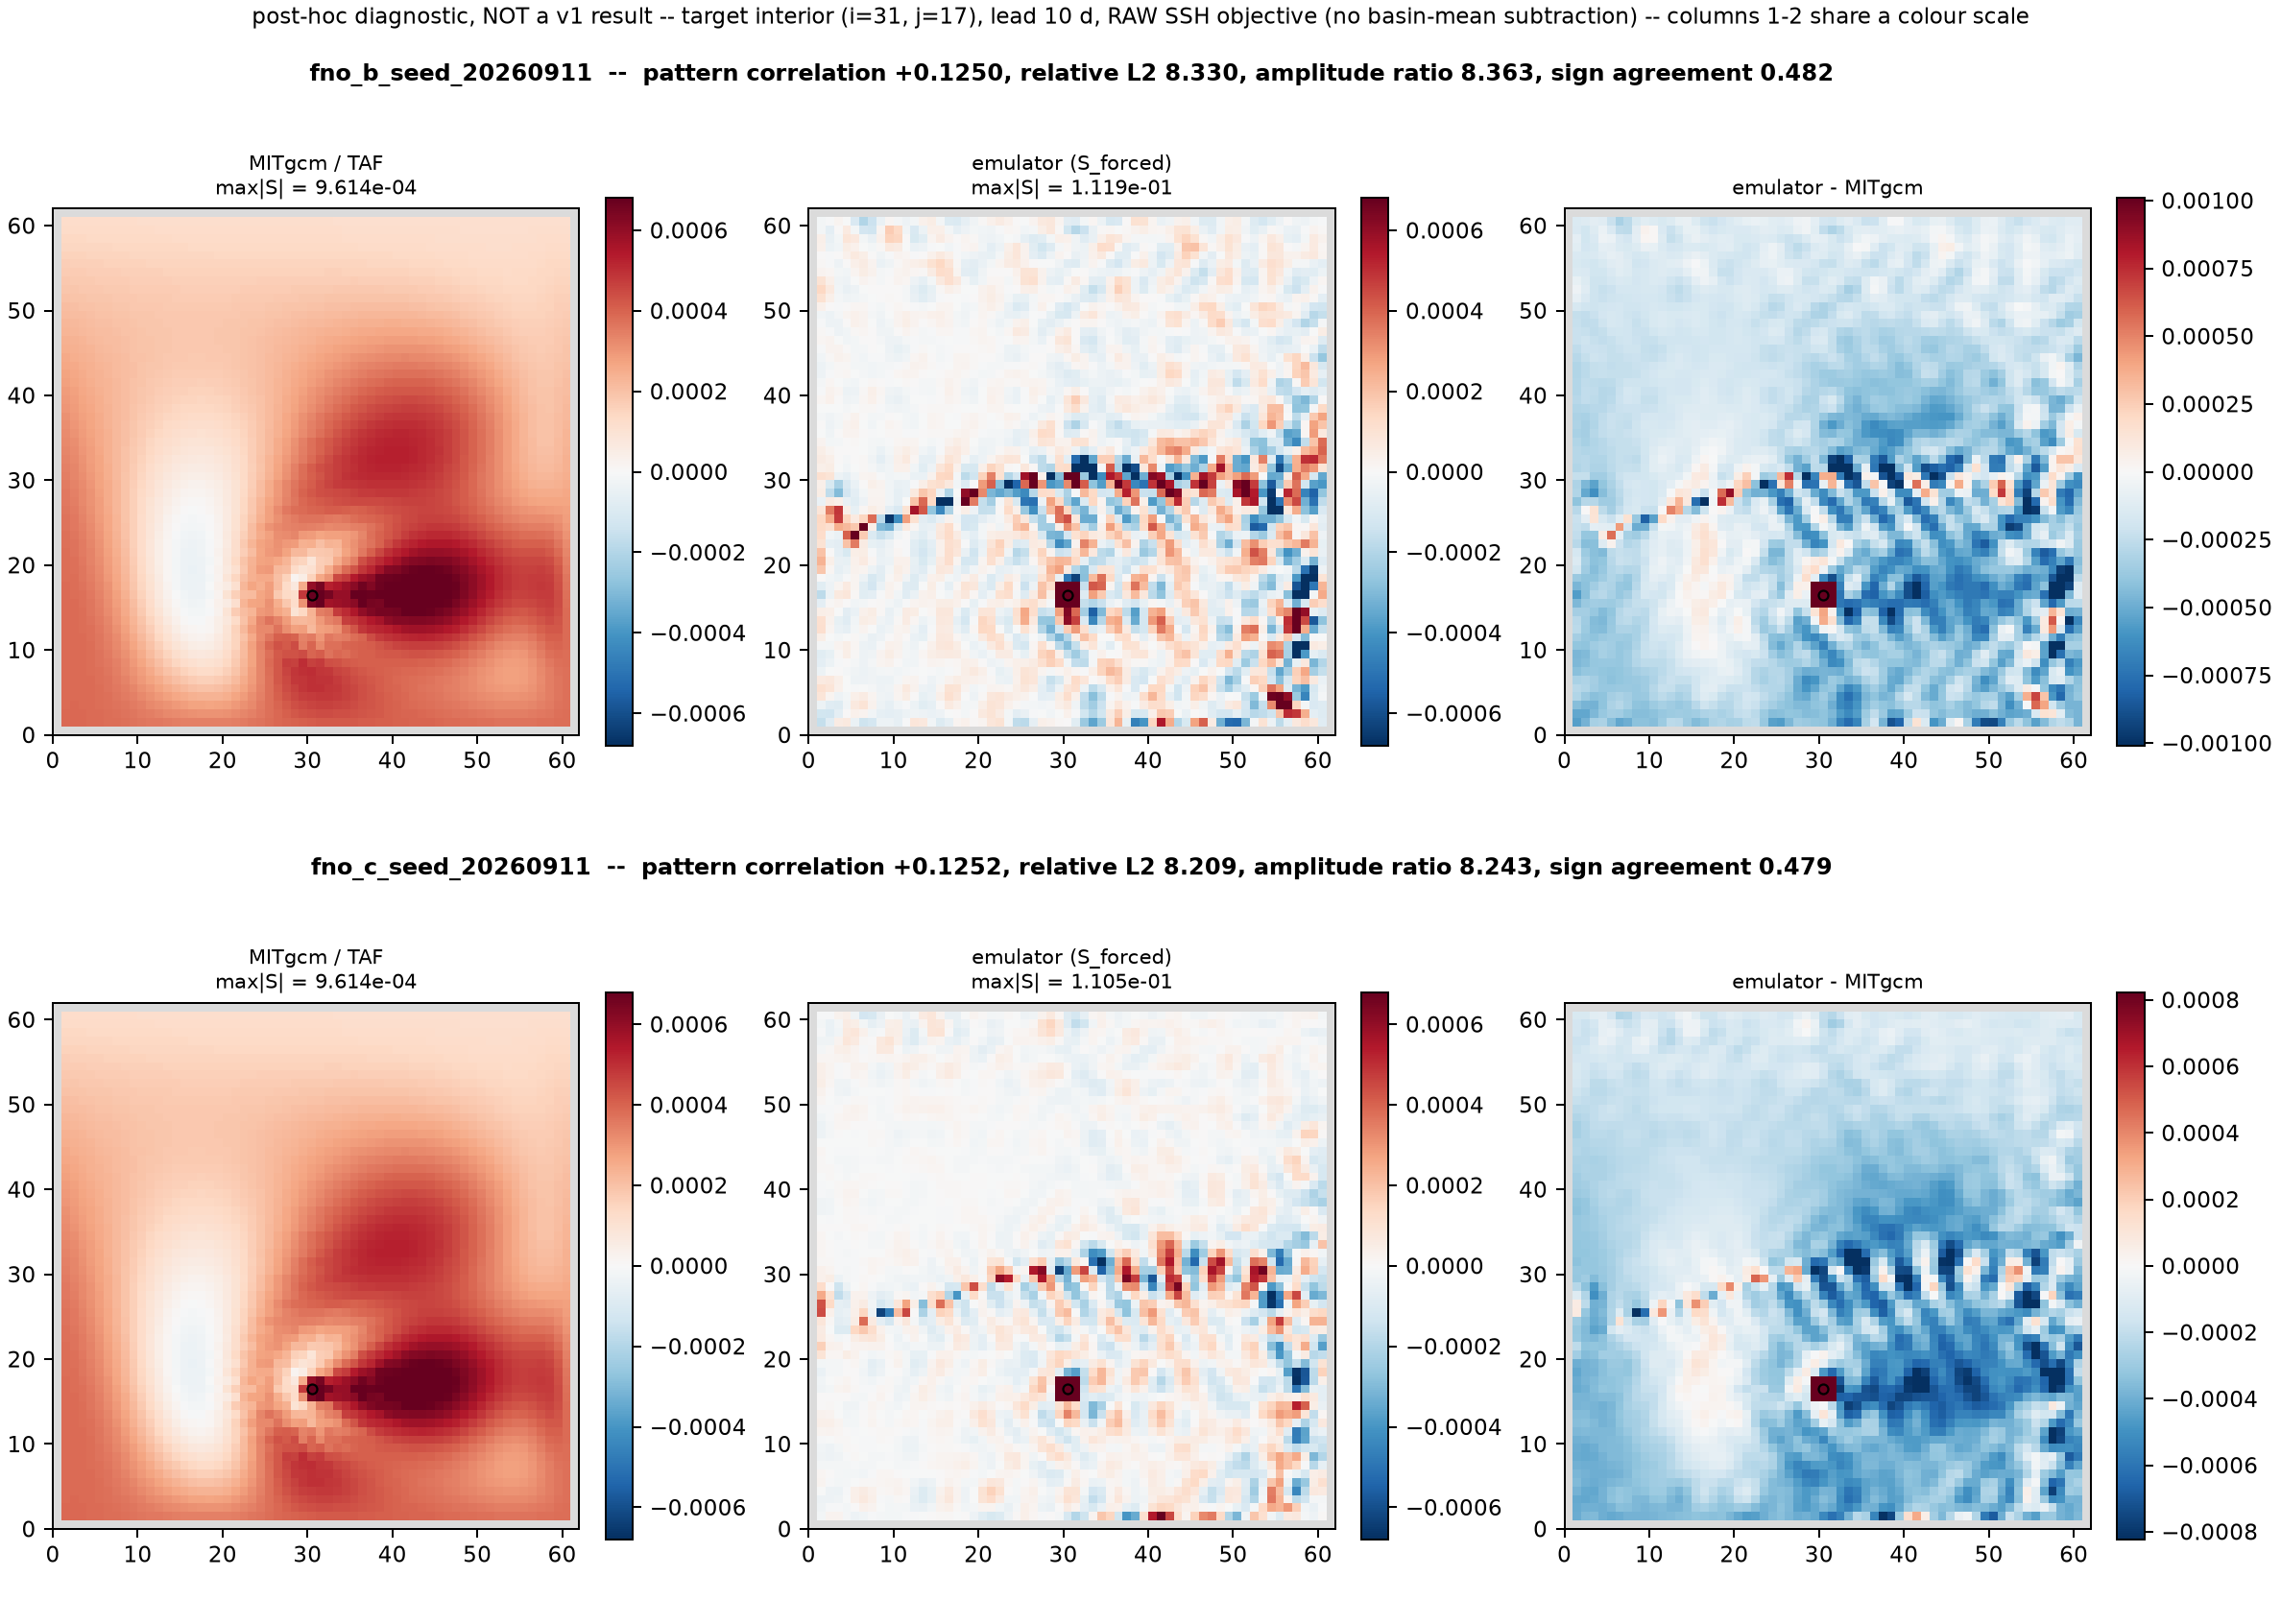
\includegraphics[width=\textwidth]{figures/adj_interior_raw_ssh_010.png}
\caption{Interior target, $J_{\mathrm{raw}}$, lead 10~d. \MITgcm{}'s sensitivity
is already basin-wide; the emulator's is a near-delta at the target plus
jet-axis speckle, 116$\times$ too large at its peak.}
\label{fig:int_raw010}
\end{figure}

\begin{figure}[htbp]
\centering
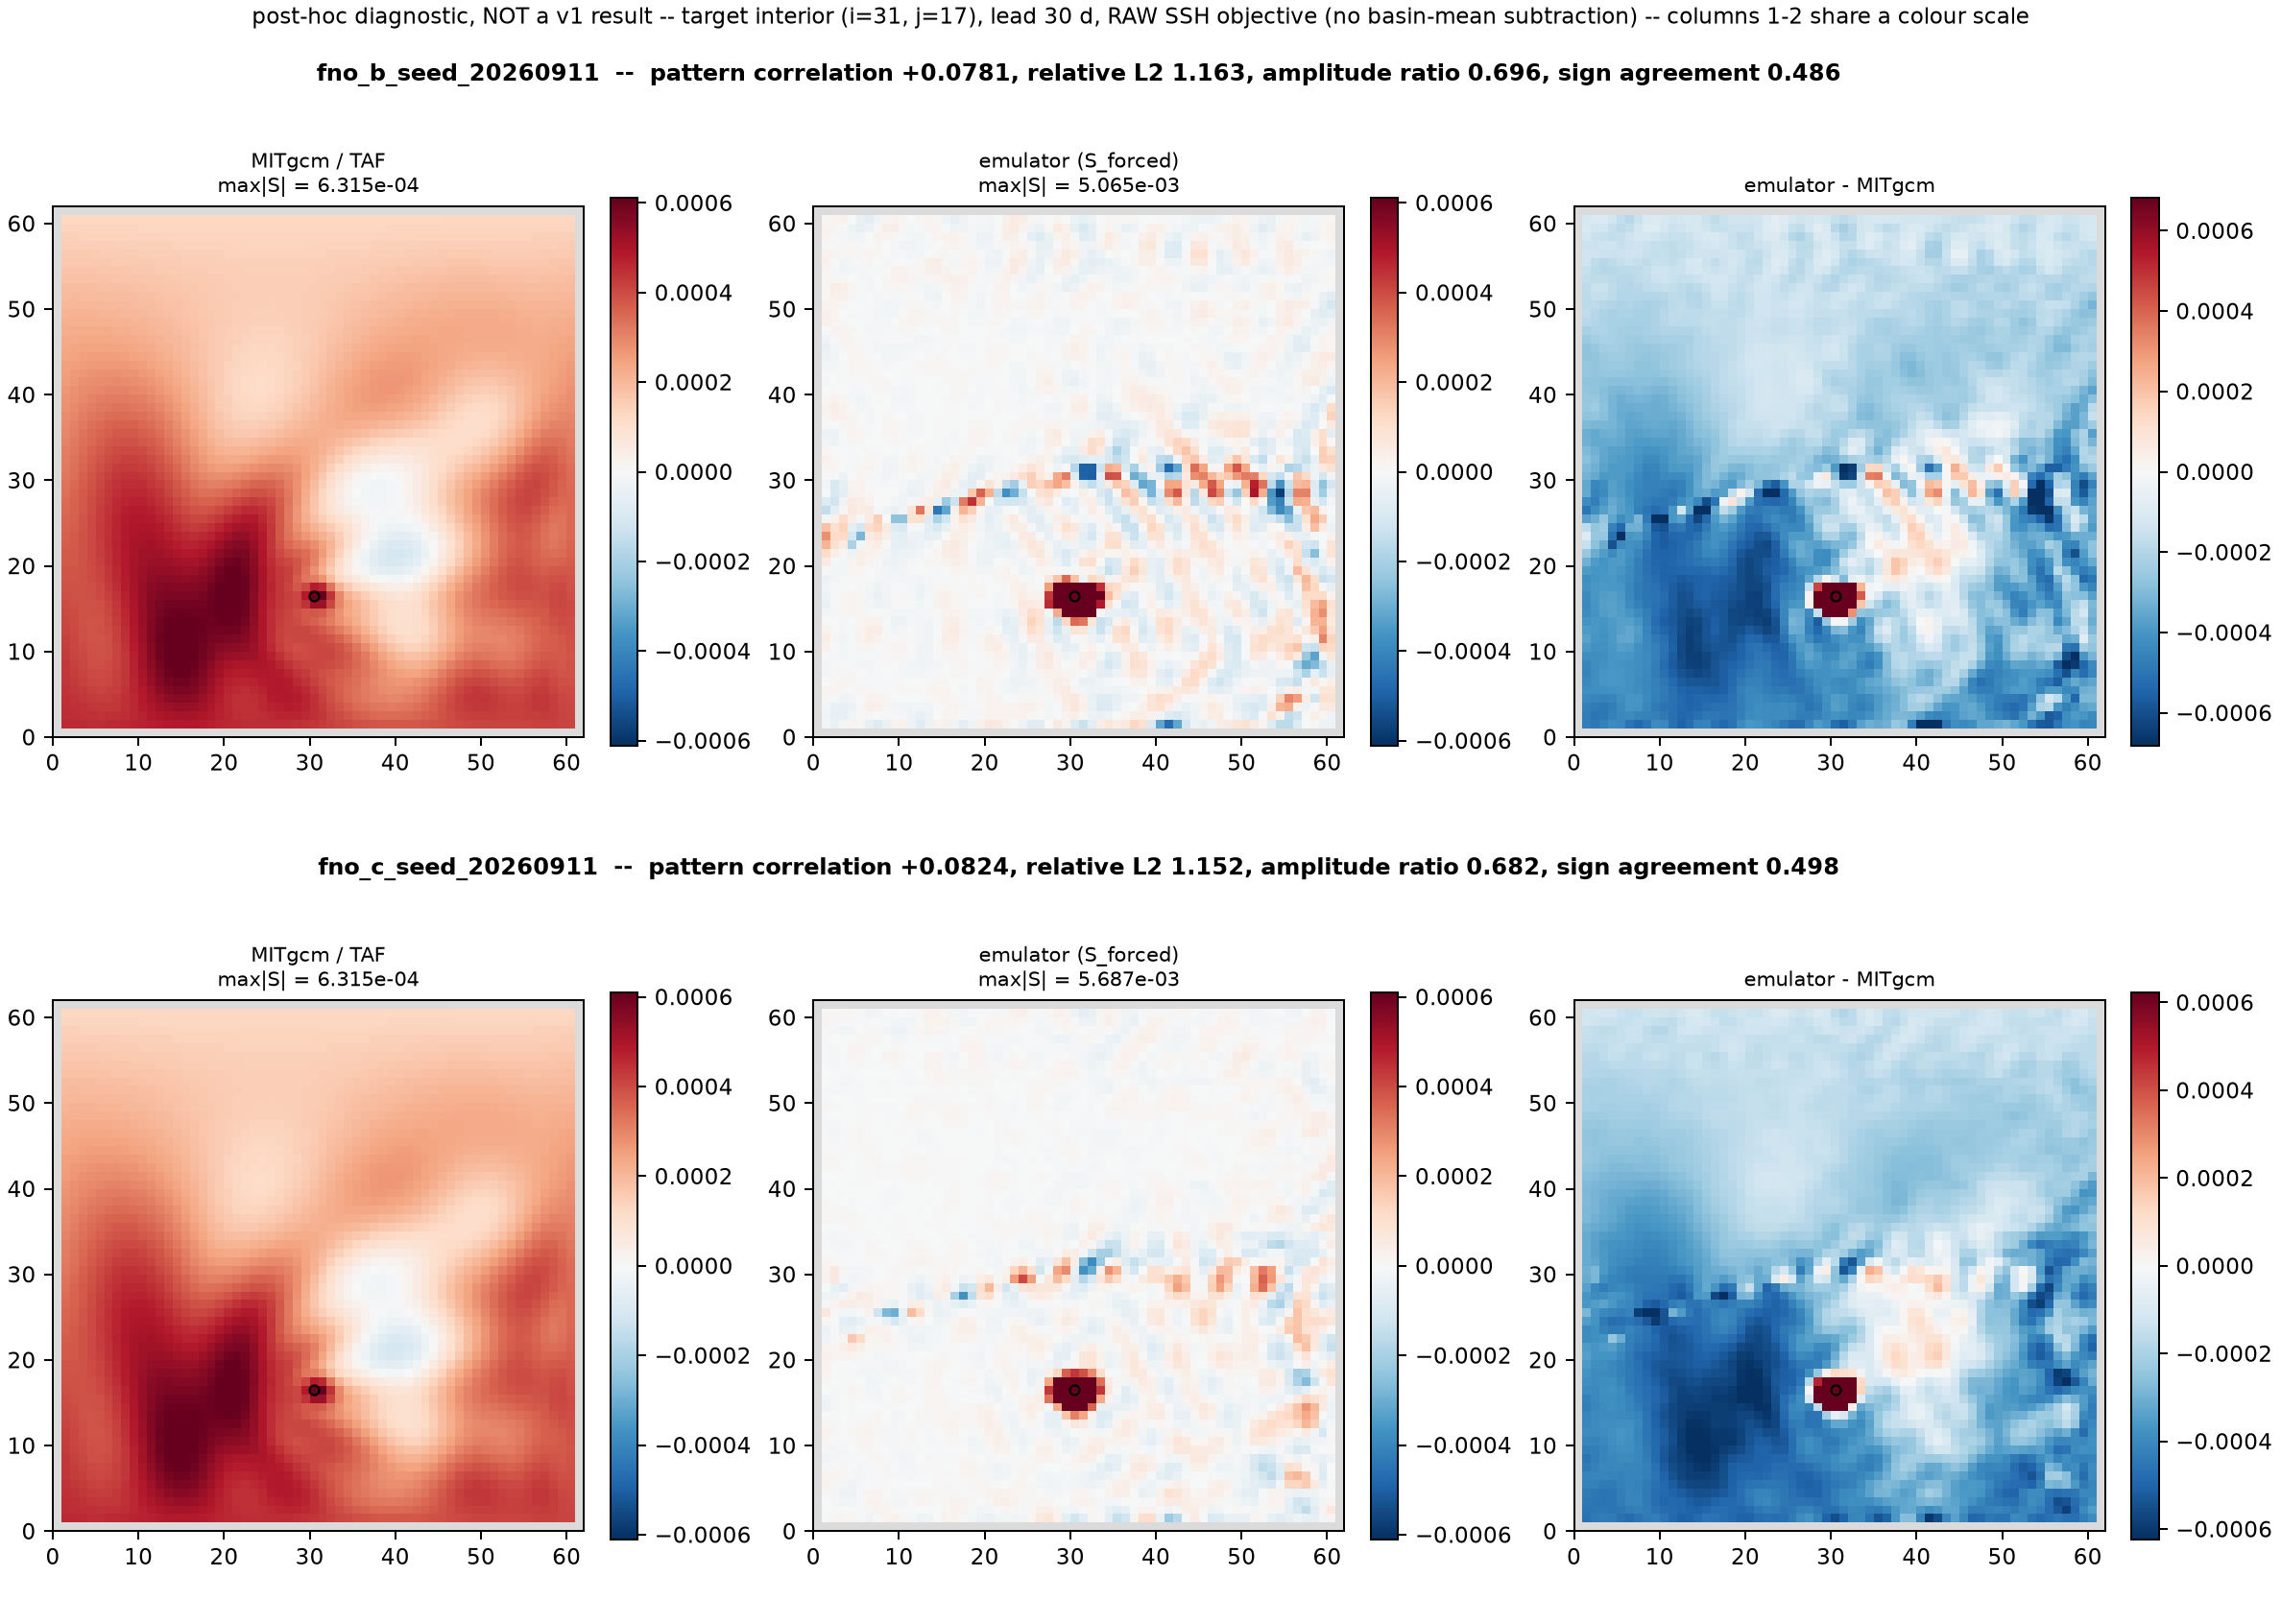
\includegraphics[width=\textwidth]{figures/adj_interior_raw_ssh_030.png}
\caption{Interior target, $J_{\mathrm{raw}}$, lead 30~d. The amplitudes have
crossed: the true sensitivity keeps growing, the emulator's decays, giving
$\alpha\approx0.69$.}
\label{fig:int_raw030}
\end{figure}

\begin{figure}[htbp]
\centering
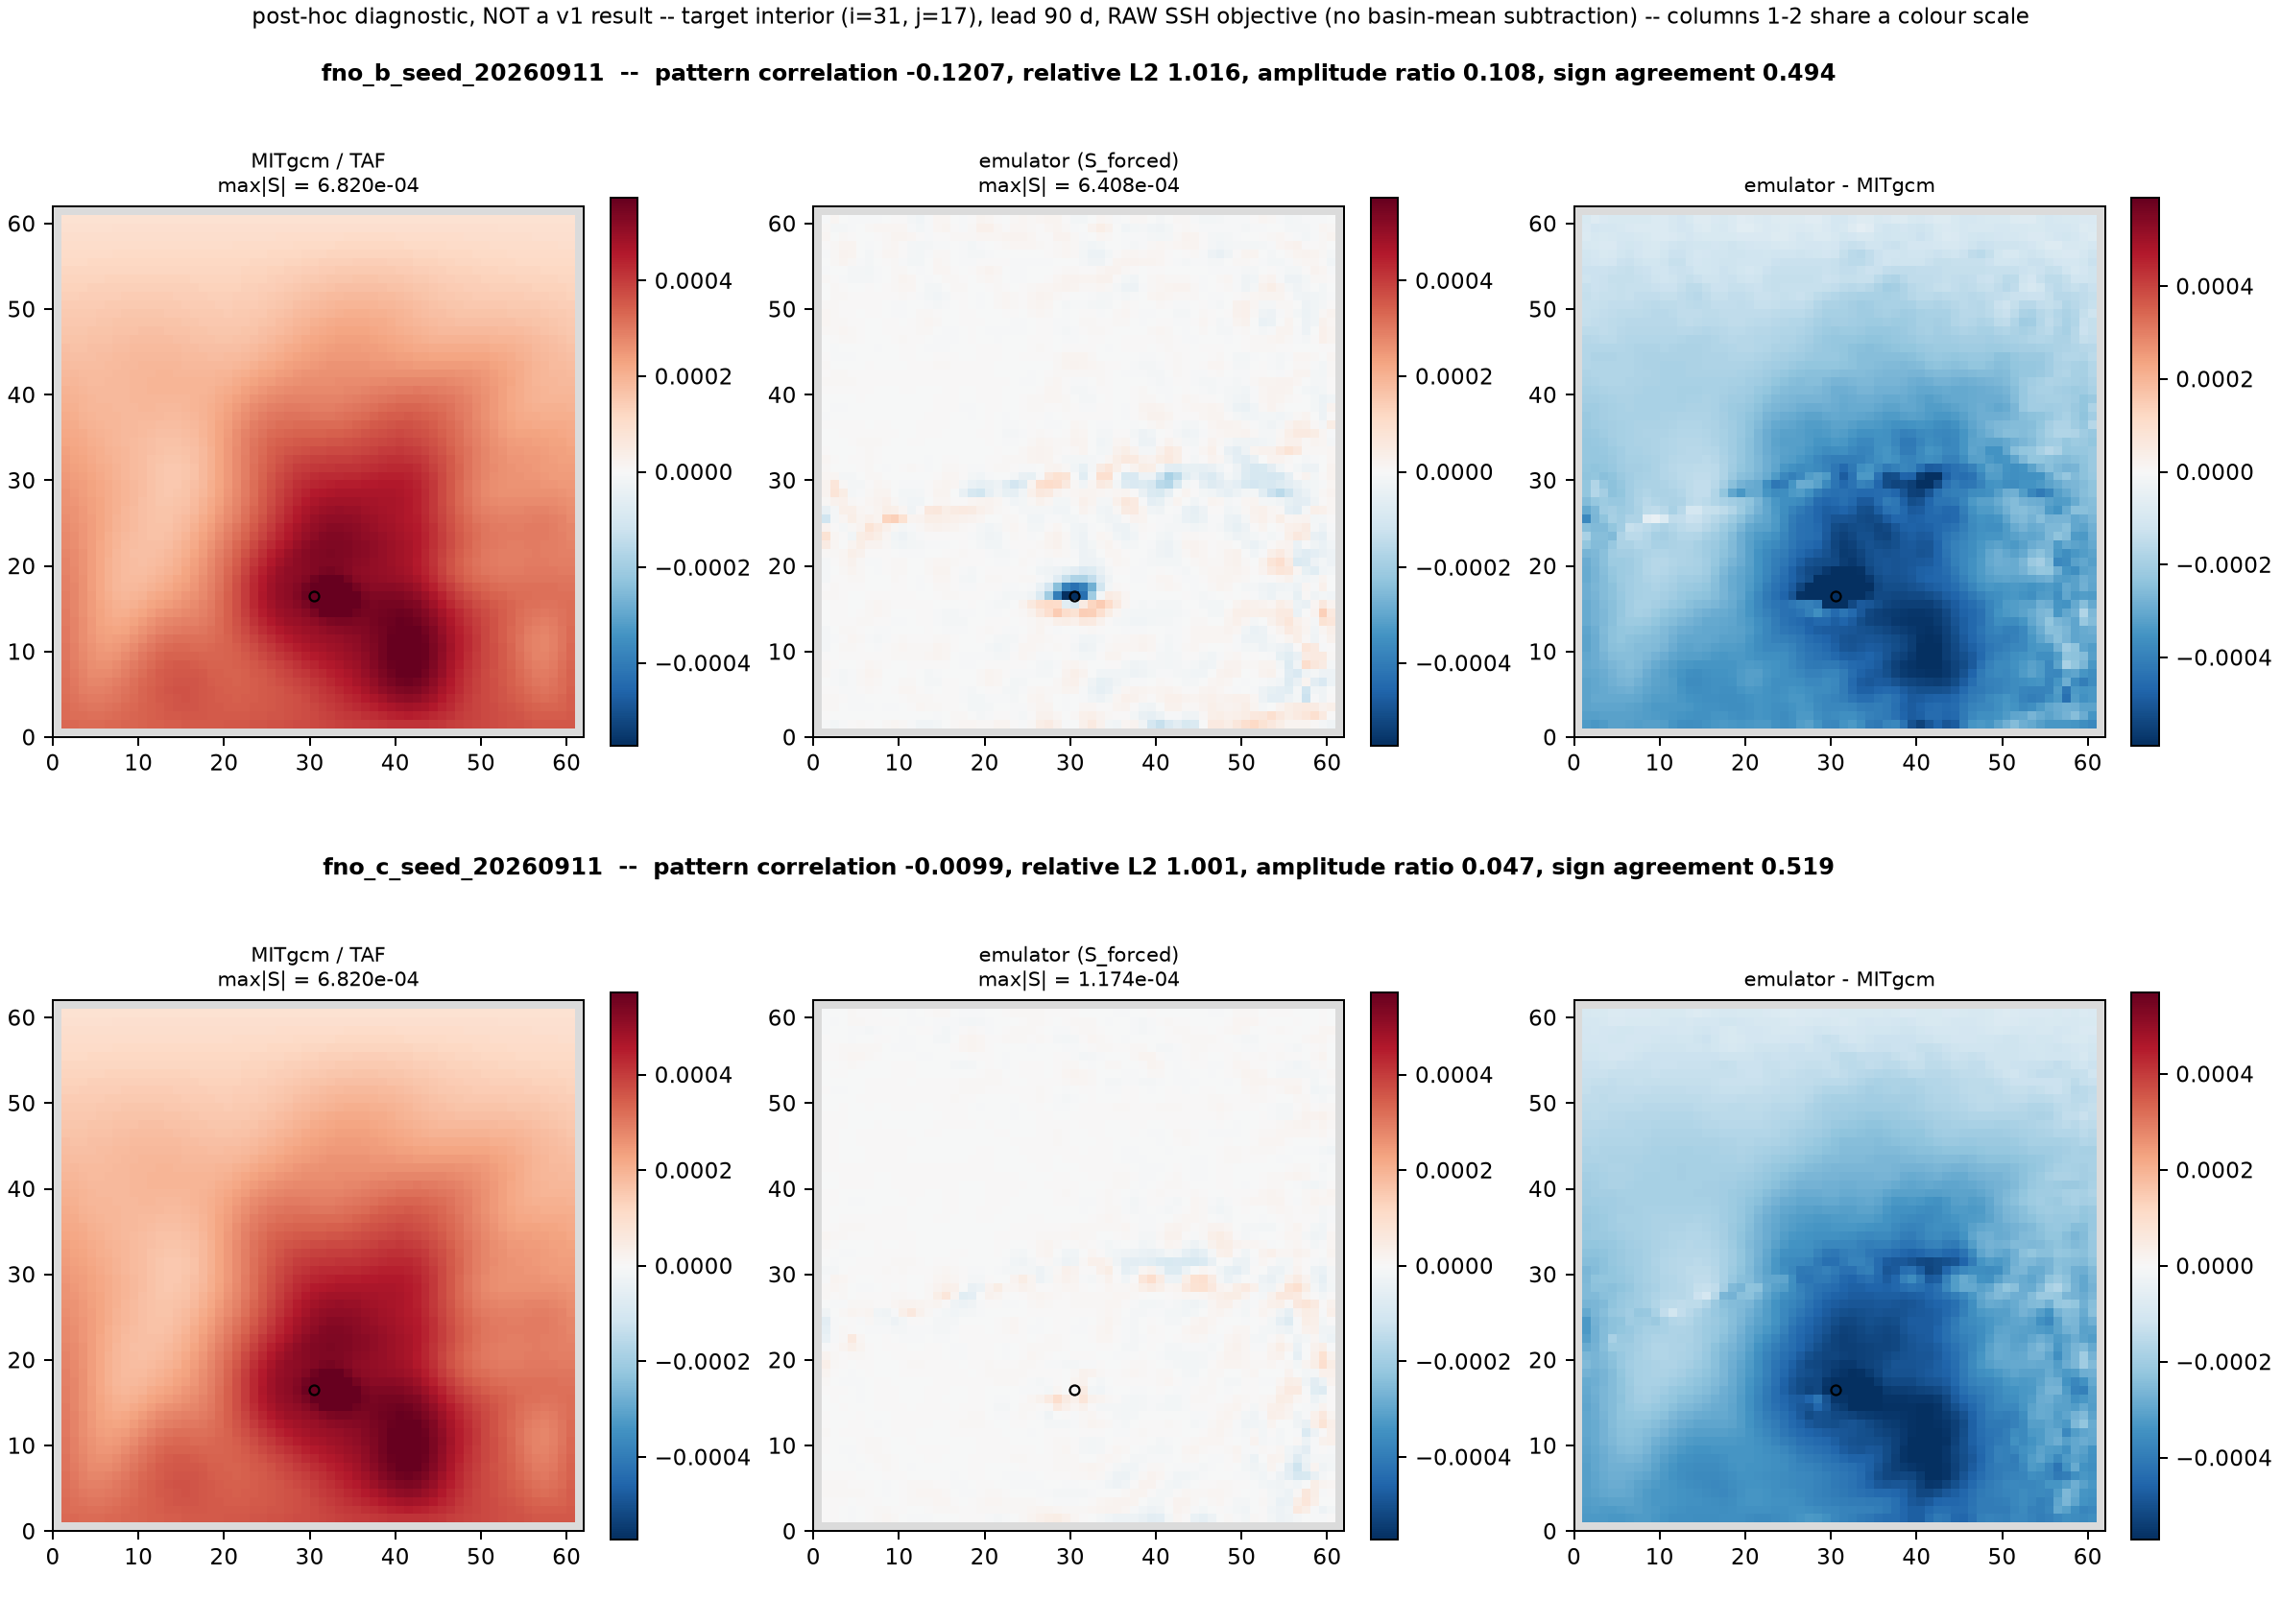
\includegraphics[width=\textwidth]{figures/adj_interior_raw_ssh_090.png}
\caption{Interior target, $J_{\mathrm{raw}}$, lead 90~d. The emulator retains
4--11\% of the true amplitude and the correlation has turned slightly negative.}
\label{fig:int_raw090}
\end{figure}

\begin{figure}[htbp]
\centering
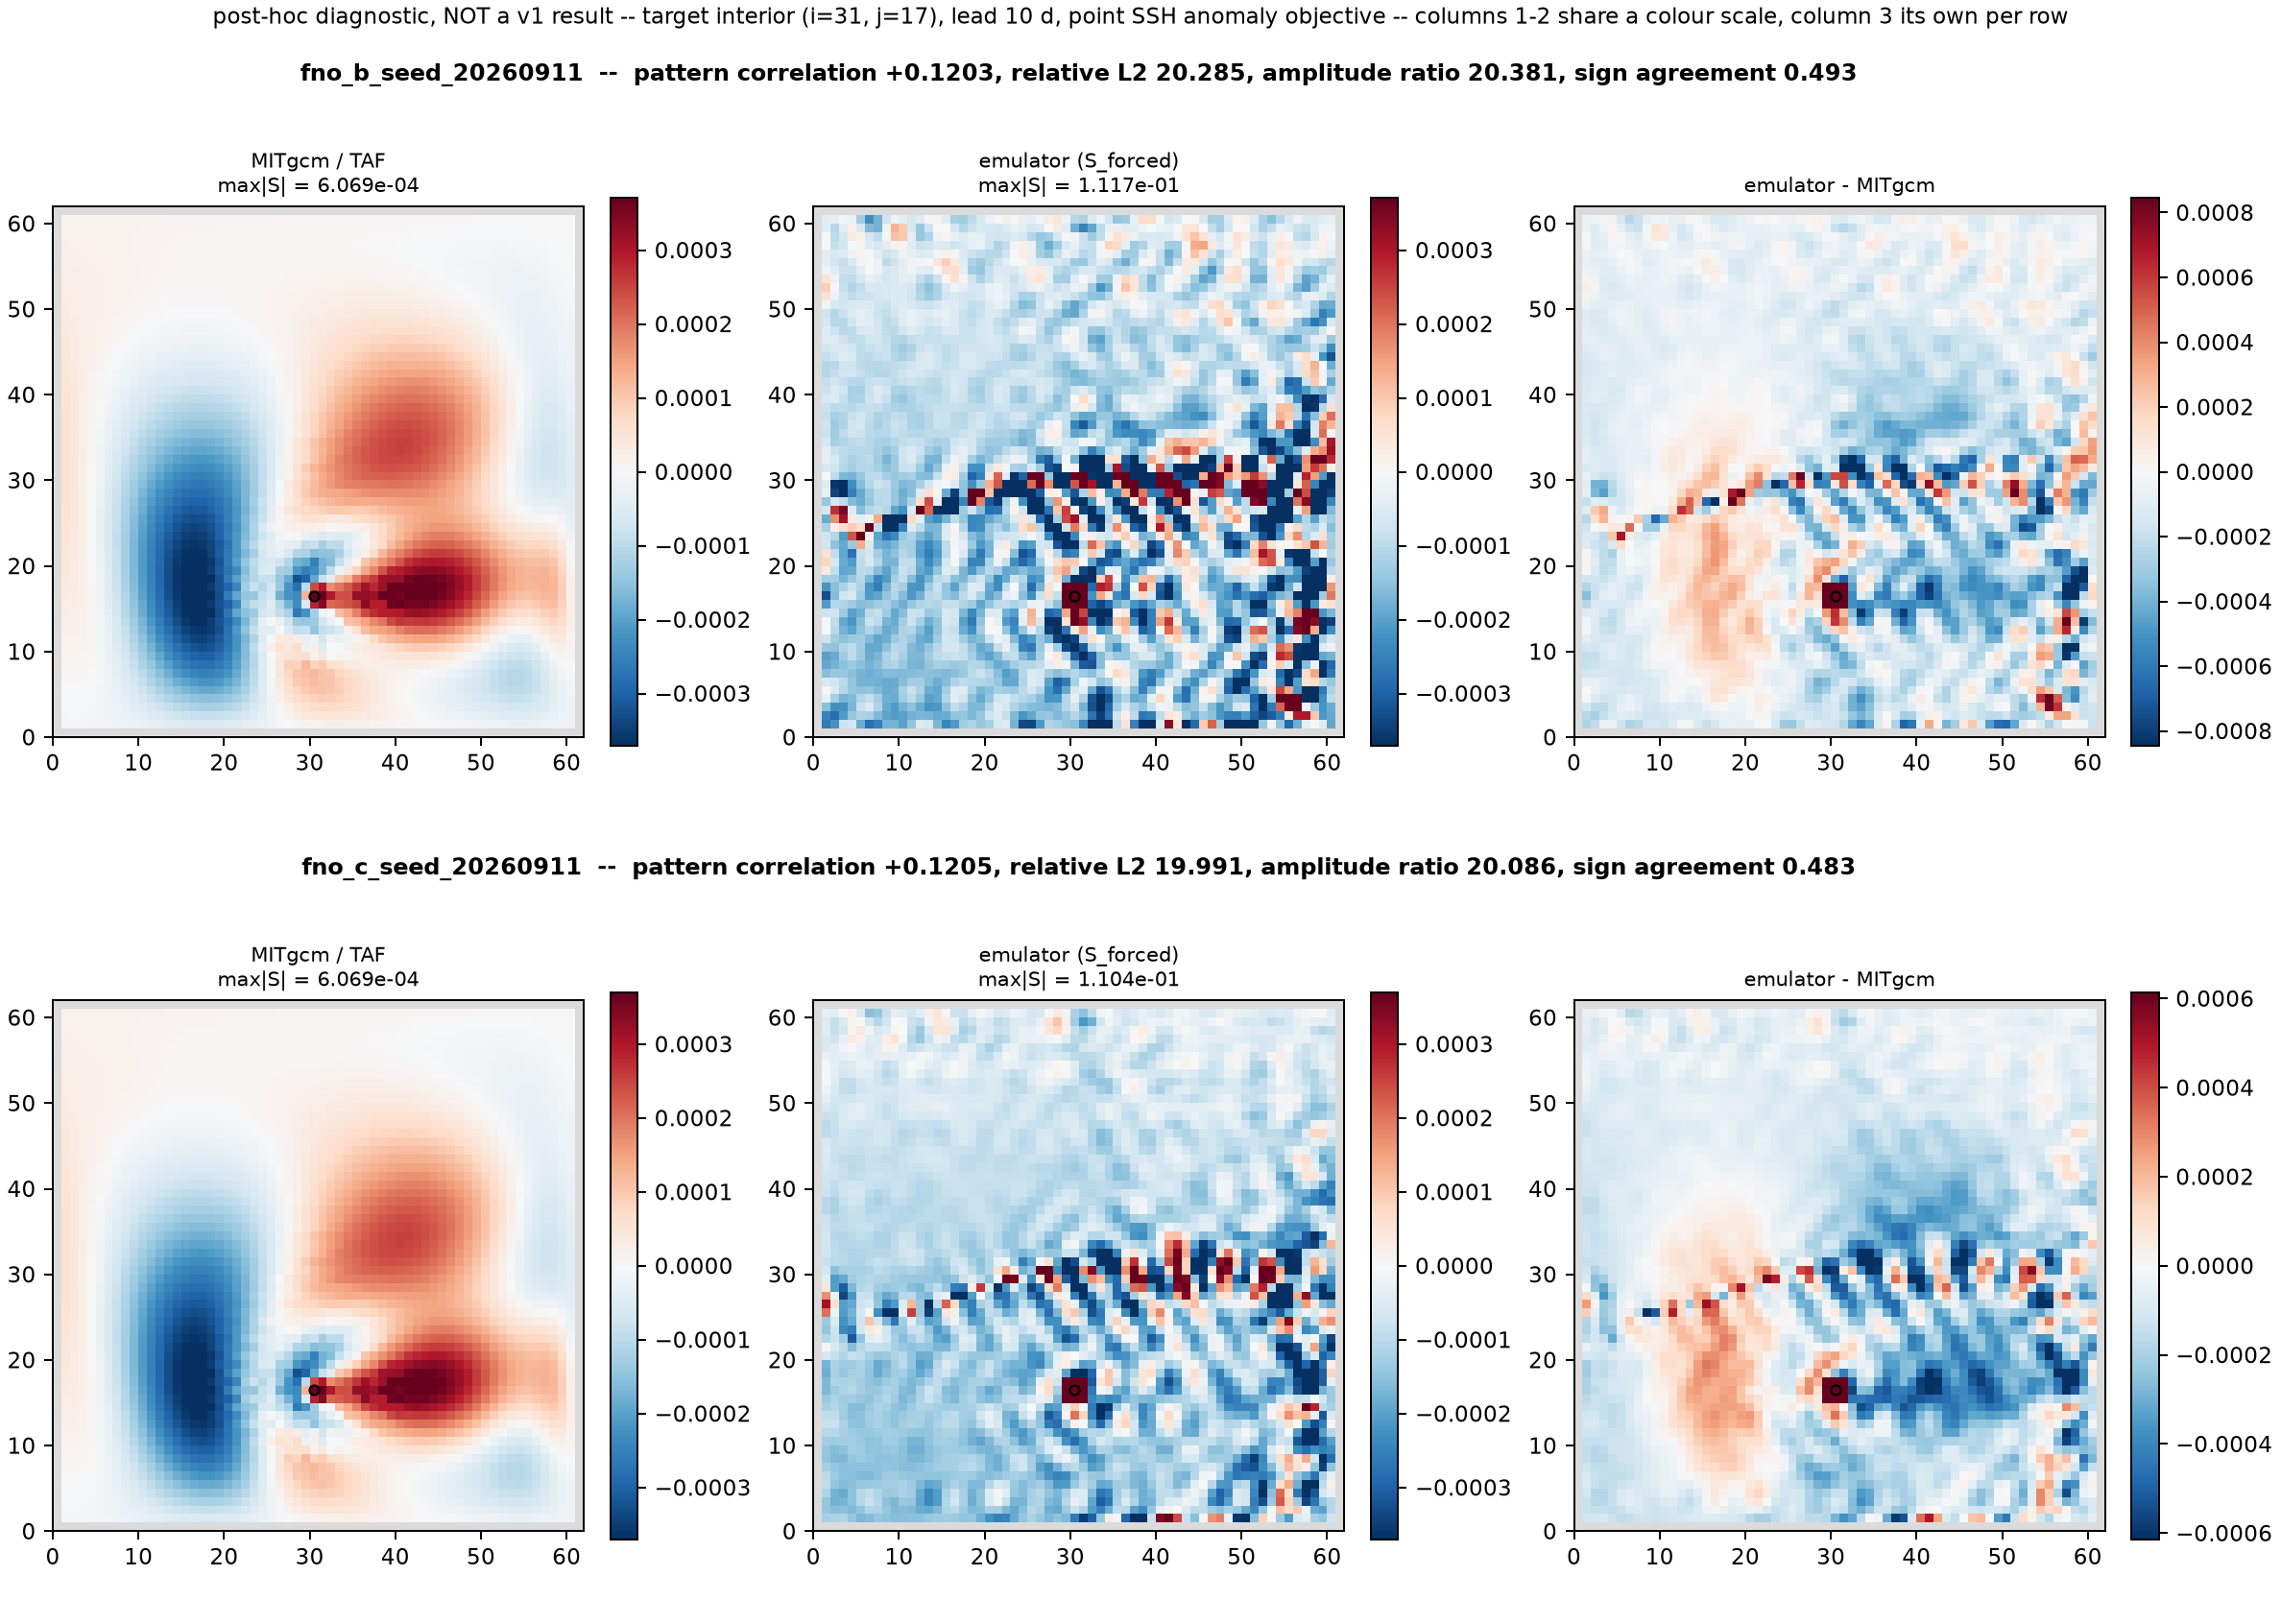
\includegraphics[width=\textwidth]{figures/adj_interior_ssh_anomaly_010.png}
\caption{Interior target, $J_{\mathrm{anom}}$, lead 10~d. With the conserved
pedestal removed the reference norm is smaller, so the same emulator error
registers as $\alpha\approx20$.}
\label{fig:int_anom010}
\end{figure}

\begin{figure}[htbp]
\centering
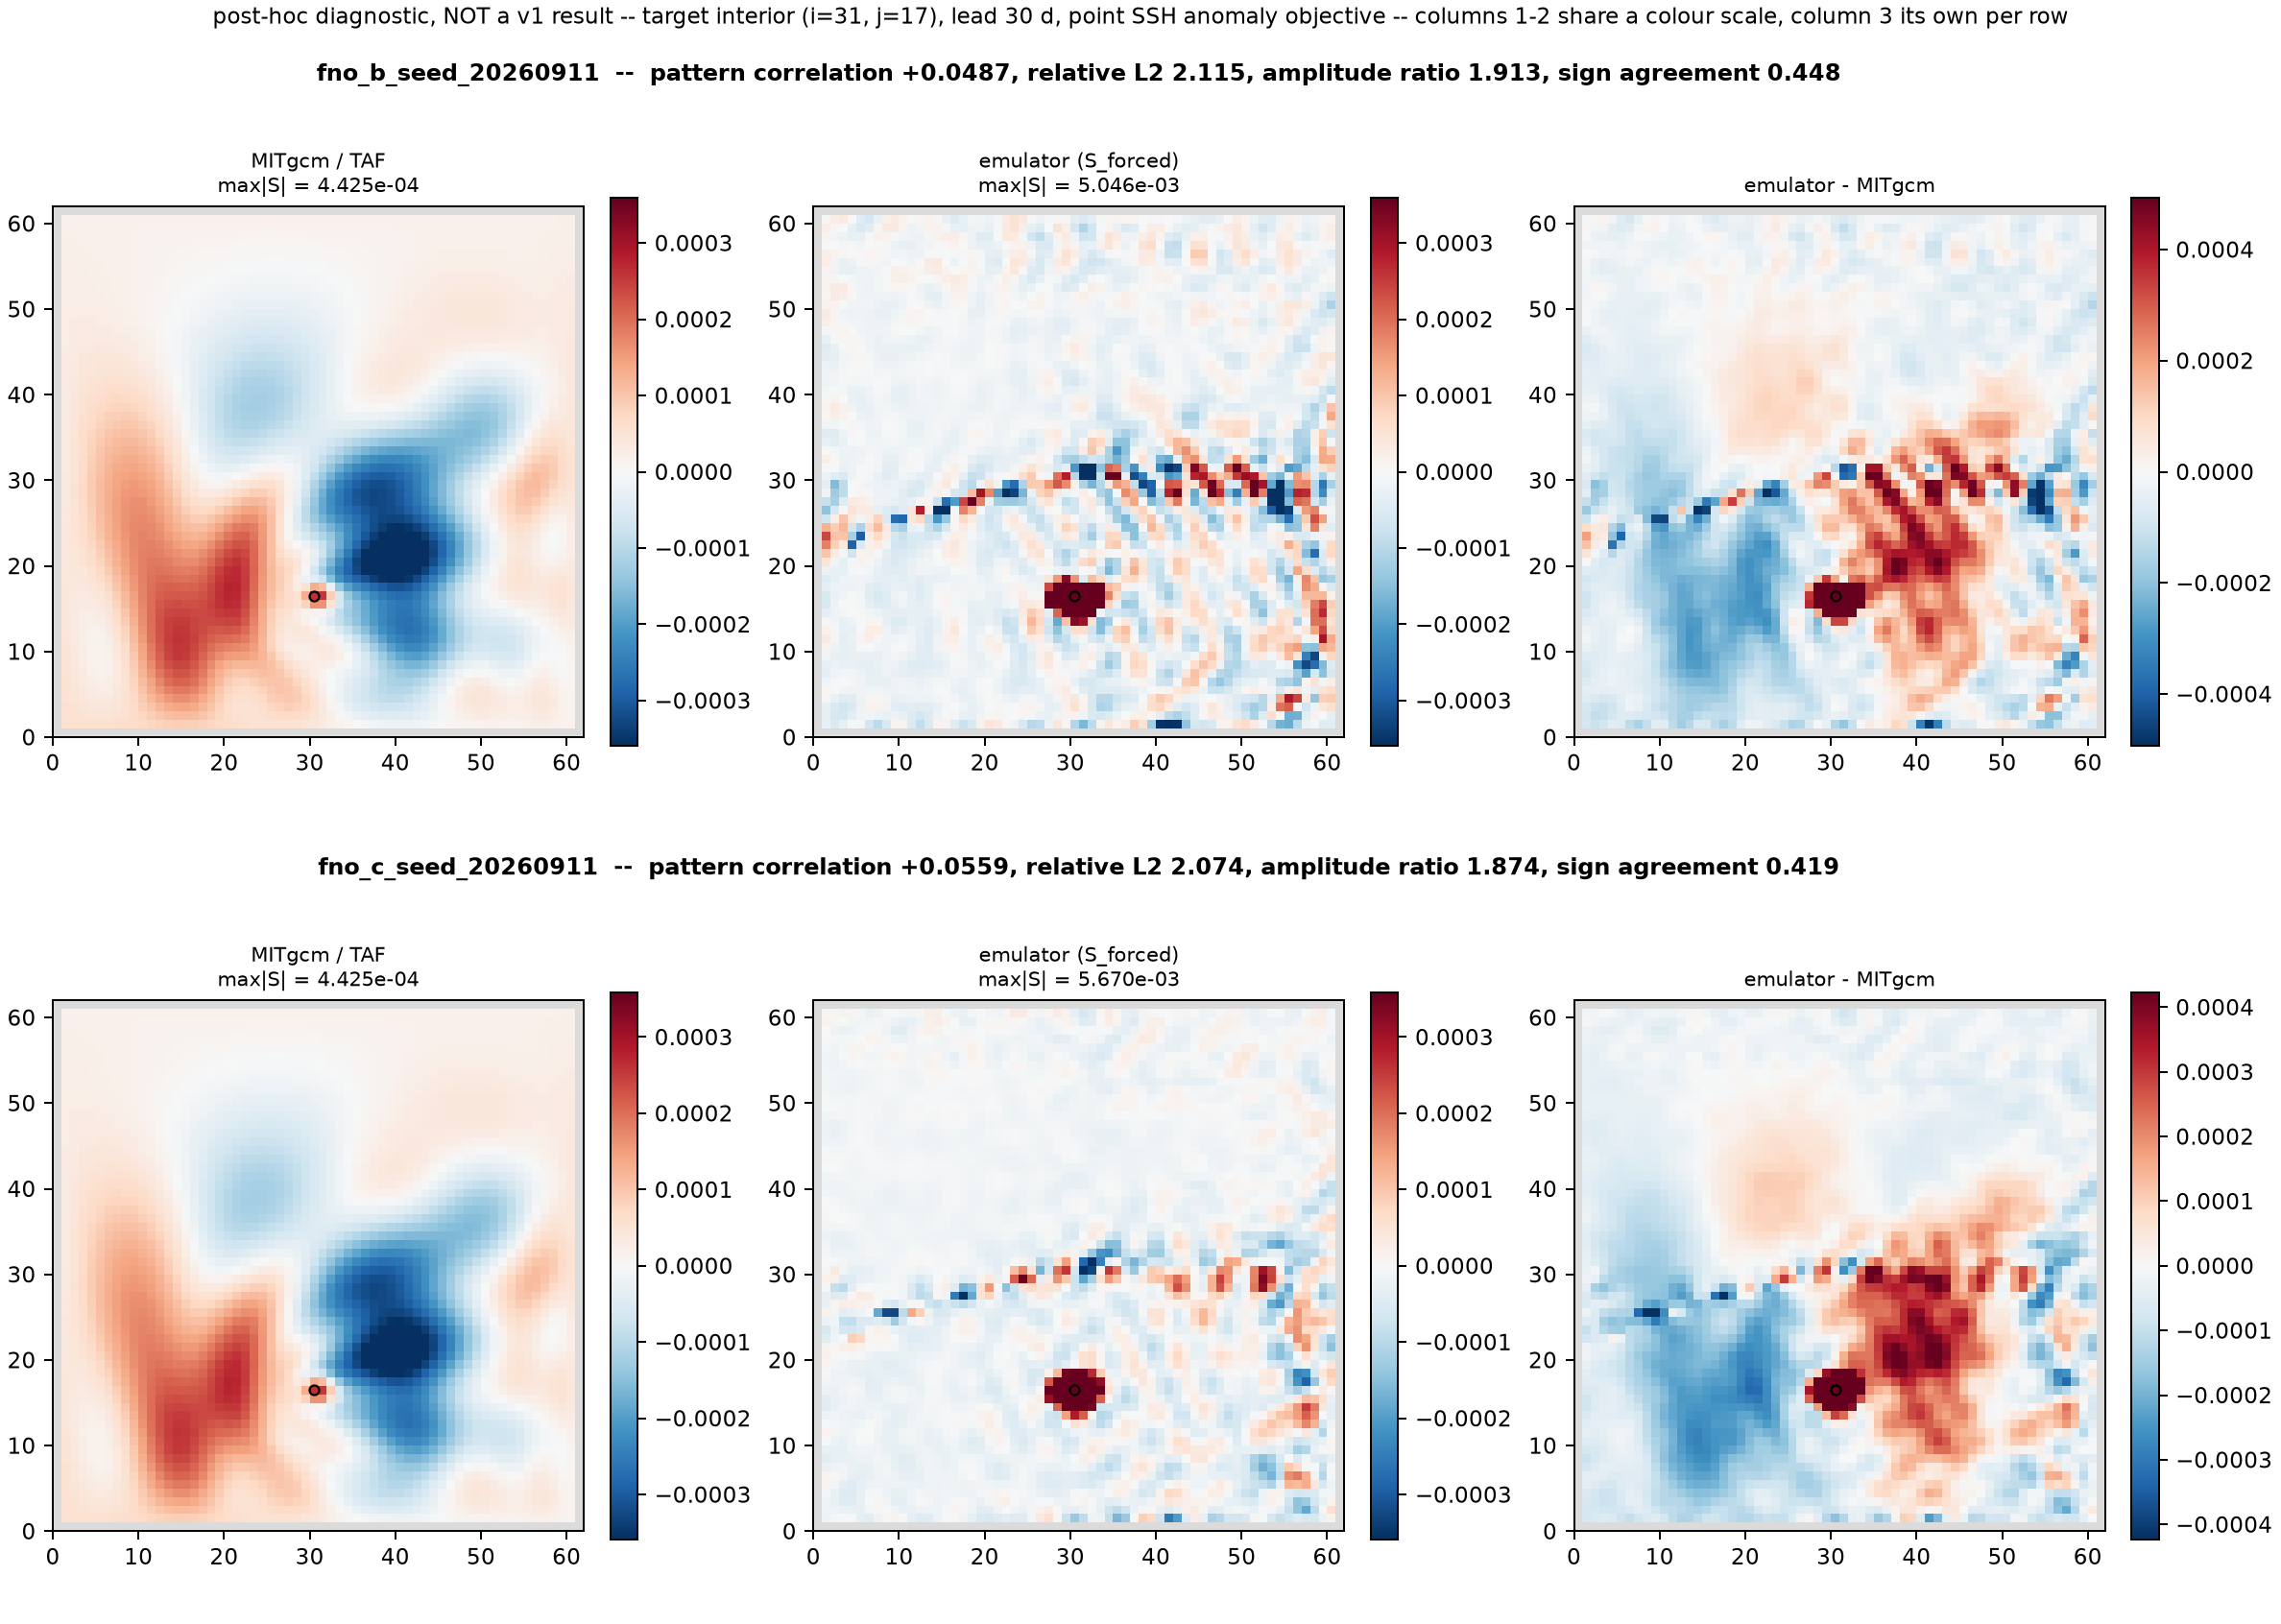
\includegraphics[width=\textwidth]{figures/adj_interior_ssh_anomaly_030.png}
\caption{Interior target, $J_{\mathrm{anom}}$, lead 30~d.}
\label{fig:int_anom030}
\end{figure}

\begin{figure}[htbp]
\centering
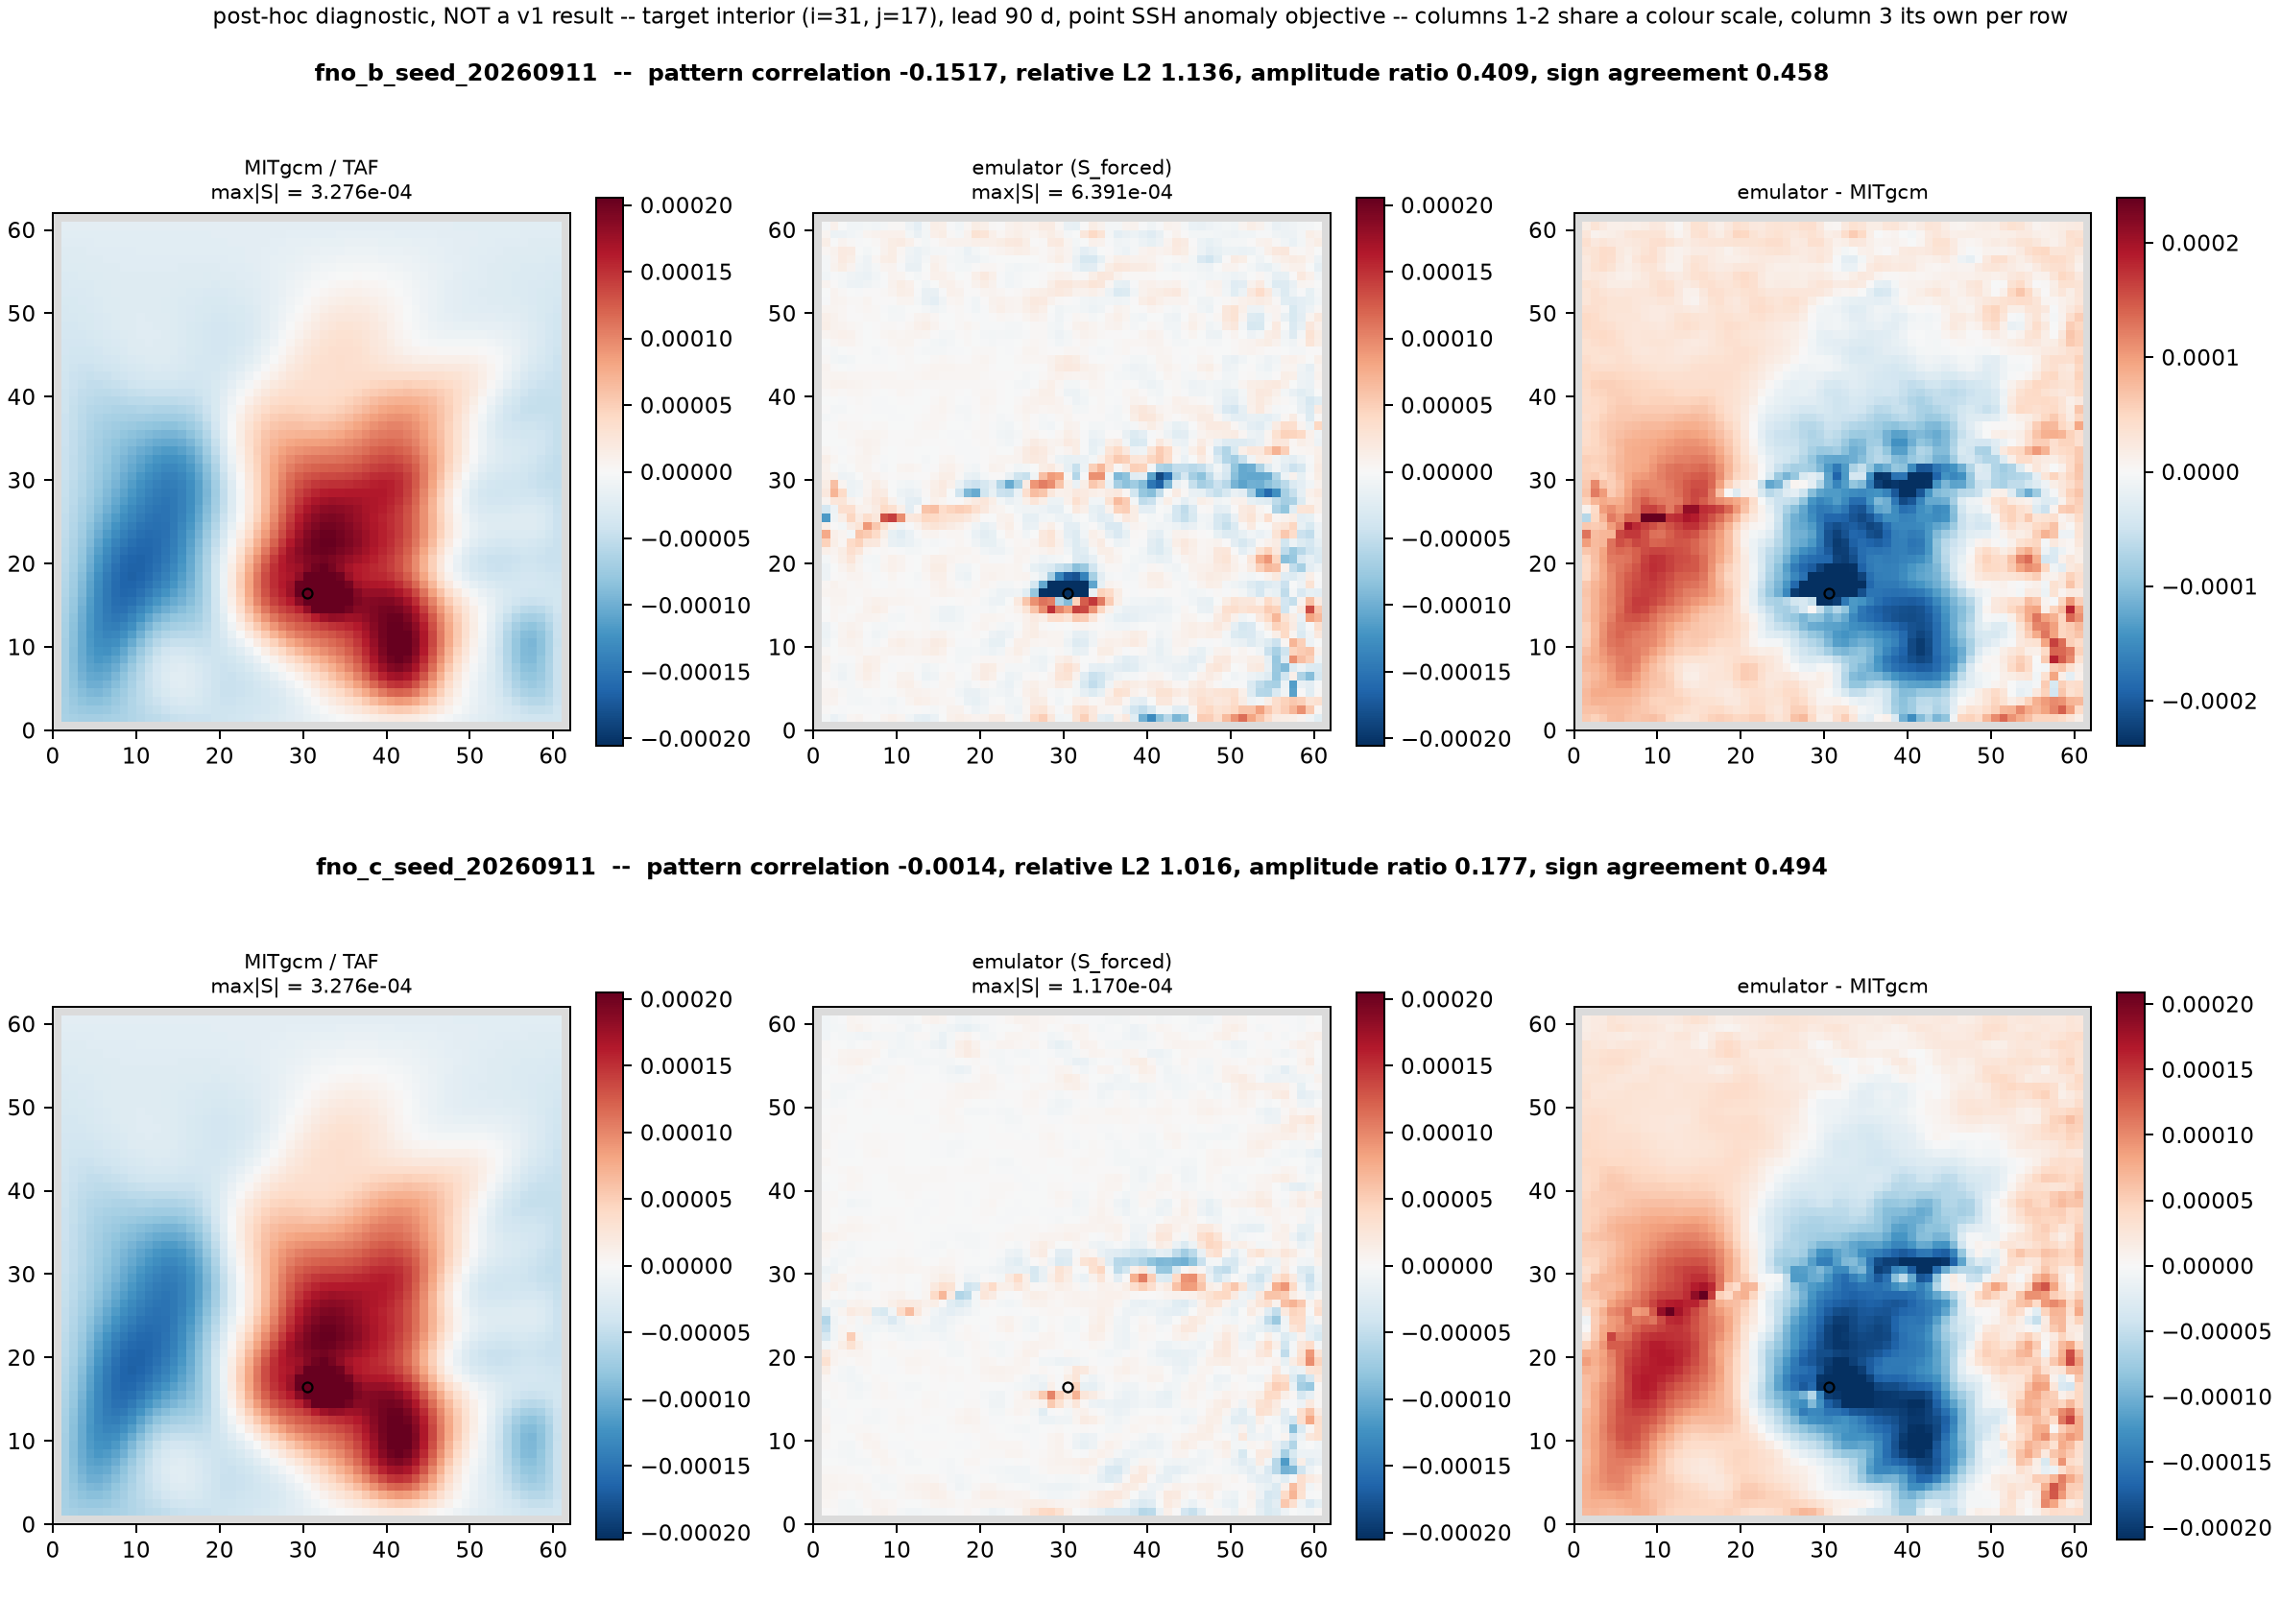
\includegraphics[width=\textwidth]{figures/adj_interior_ssh_anomaly_090.png}
\caption{Interior target, $J_{\mathrm{anom}}$, lead 90~d. The true map is a
clean two-lobed Rossby-propagation pattern; neither emulator reproduces any part
of it.}
\label{fig:int_anom090}
\end{figure}

\subsubsection{Eastern target}
\label{sec:eastern}

The eastern target sits at $(61,17)$, in the last wet column against the eastern
wall.

\begin{table}[H]
\centering
\small
\begin{tabular}{llrrrrrr}
\toprule
& & \multicolumn{3}{c}{Control} & \multicolumn{3}{c}{Response} \\
\cmidrule(lr){3-5}\cmidrule(lr){6-8}
Objective & Lead (d) & $\rho$ & $\varepsilon_2$ & $\alpha$ & $\rho$ & $\varepsilon_2$ & $\alpha$ \\
\midrule
$J_{\mathrm{raw}}$  & 10 & $+0.109$ & 10.213 & 10.243 & $+0.108$ & \textbf{9.835} & 9.863 \\
$J_{\mathrm{raw}}$  & 30 & $+0.109$ & 1.257 & 0.857 & $+0.106$ & \textbf{1.232} & 0.810 \\
$J_{\mathrm{raw}}$  & 90 & $-0.016$ & 1.004 & 0.087 & $+0.037$ & \textbf{0.999} & 0.026 \\
$J_{\mathrm{anom}}$ & 10 & $+0.178$ & 47.016 & 47.183 & $+0.177$ & \textbf{45.265} & 45.431 \\
$J_{\mathrm{anom}}$ & 30 & $+0.154$ & 6.633 & 6.713 & $+0.154$ & \textbf{6.264} & 6.339 \\
$J_{\mathrm{anom}}$ & 90 & $-0.034$ & 1.466 & 1.038 & $-0.014$ & \textbf{1.051} & 0.311 \\
\bottomrule
\end{tabular}
\caption{Eastern target $(61,17)$. The response arm again has the lower relative
$L_2$ in all six cells; the lead-90 anomaly cell is the largest single reduction
in this report (28\%).}
\label{tab:eastern}
\end{table}

\paragraph{Discussion} The eastern target produces the largest amplitude errors
in the study --- 47$\times$ at lead 10 under $J_{\mathrm{anom}}$ --- and also
the highest pattern correlations, $+0.18$. Both facts have the same cause. The
true lead-10 anomaly sensitivity (Figure~\ref{fig:east_anom010}) is a smooth,
large-scale dipole: strongly positive over the entire south-western quadrant,
negative through a broad lobe centred near $(42,20)$, with a thin band of
alternating sign right against the eastern wall where the target sits. Its
overall norm is small because the field is smooth and the eastern wall is the
quietest part of the basin, so the emulator's grid-scale error dominates the
ratio. At the same time, the emulator's map is broadly negative over most of the
basin, which happens to agree in sign with a large fraction of the reference ---
hence $\sigma=0.61$, the highest sign agreement anywhere in this report, and
$\rho=+0.18$. That is coincidental large-scale bias agreement, not structural
skill: the emulator's map is dominated by a boundary-hugging spike at the target
column ($\max|S|=1.27\times10^{-1}$ against $4.5\times10^{-4}$) and by speckle
along the jet, neither of which is present in truth.

The lead-90 anomaly cell is where the response term does the most good anywhere
in this report: $\varepsilon_2$ falls from 1.466 to 1.051 and $\alpha$ from 1.038
to 0.311, a 28\% reduction. But reading the two numbers together shows what
happened. The control arm's amplitude was already almost exactly right
($\alpha=1.04$) and its correlation was $-0.03$; it had the right amount of
sensitivity in entirely the wrong places. The response arm reduced the error by
having \emph{less} sensitivity ($\alpha=0.31$), not by relocating it. That is the
generic mechanism behind the improvements in these tables, and it is why a
falling $\varepsilon_2$ alongside a flat $\rho$ should not be read as progress
toward a faithful adjoint.

\begin{figure}[htbp]
\centering
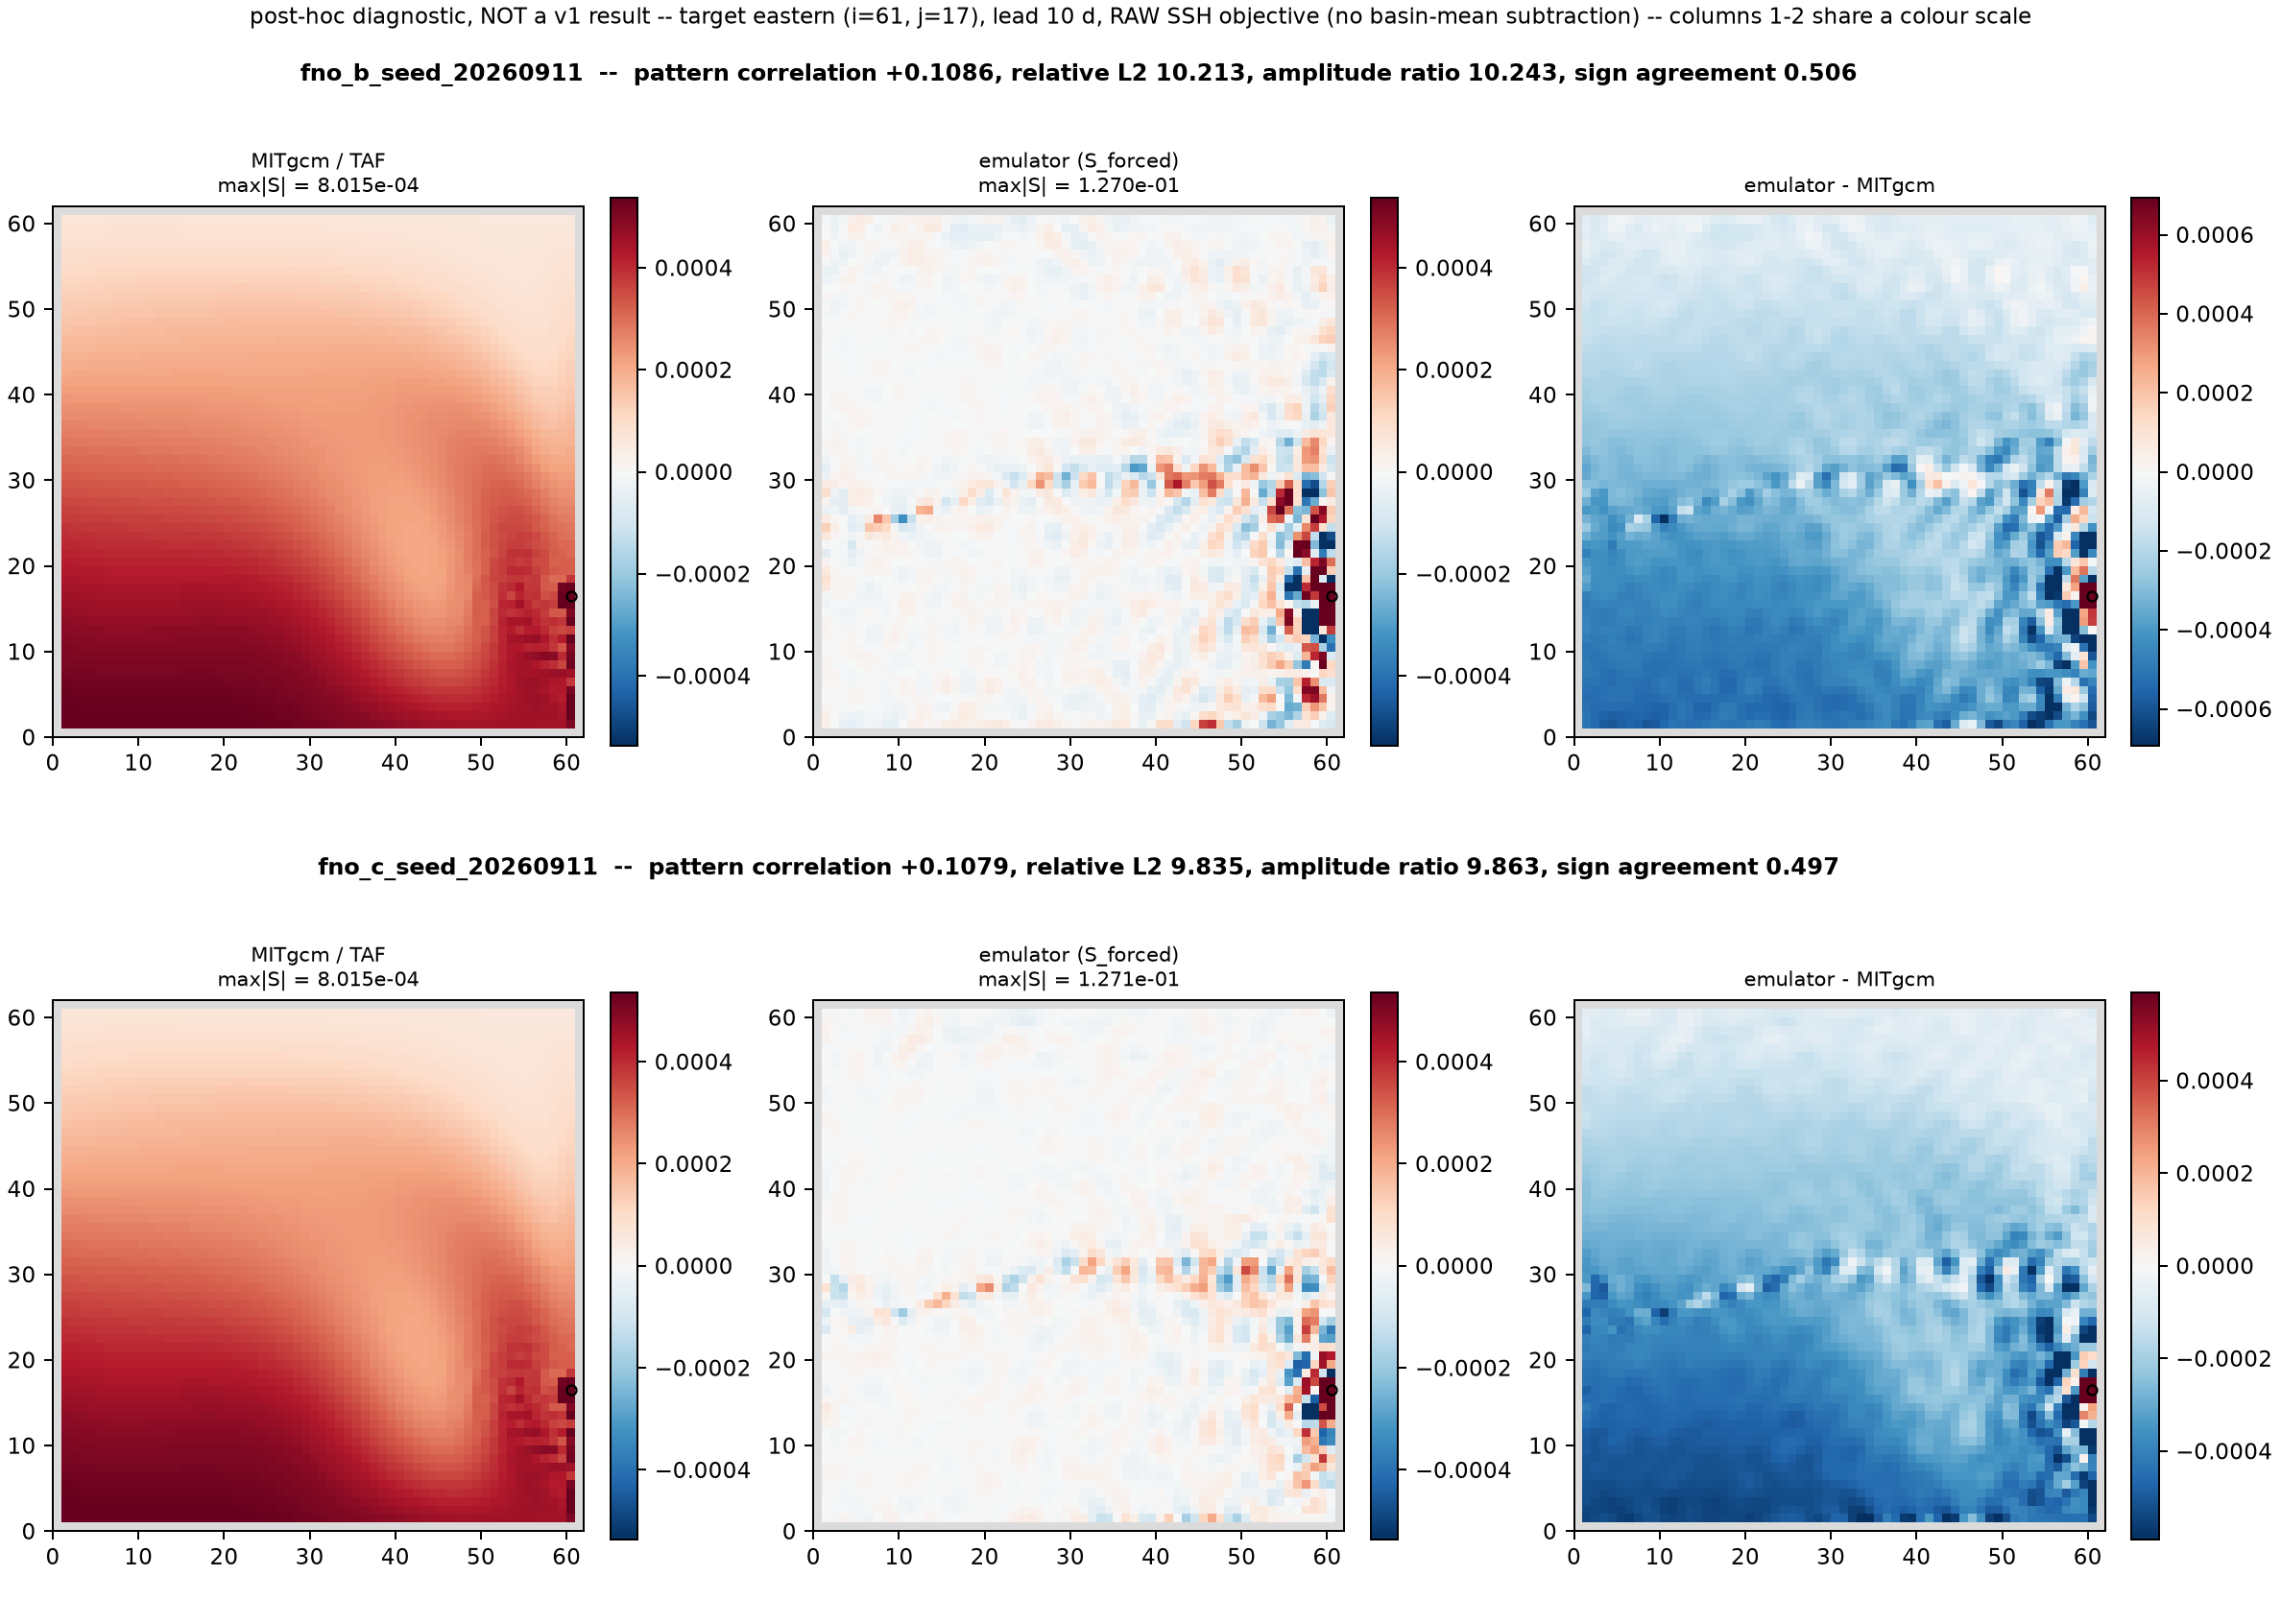
\includegraphics[width=\textwidth]{figures/adj_eastern_raw_ssh_010.png}
\caption{Eastern target, $J_{\mathrm{raw}}$, lead 10~d.}
\label{fig:east_raw010}
\end{figure}

\begin{figure}[htbp]
\centering
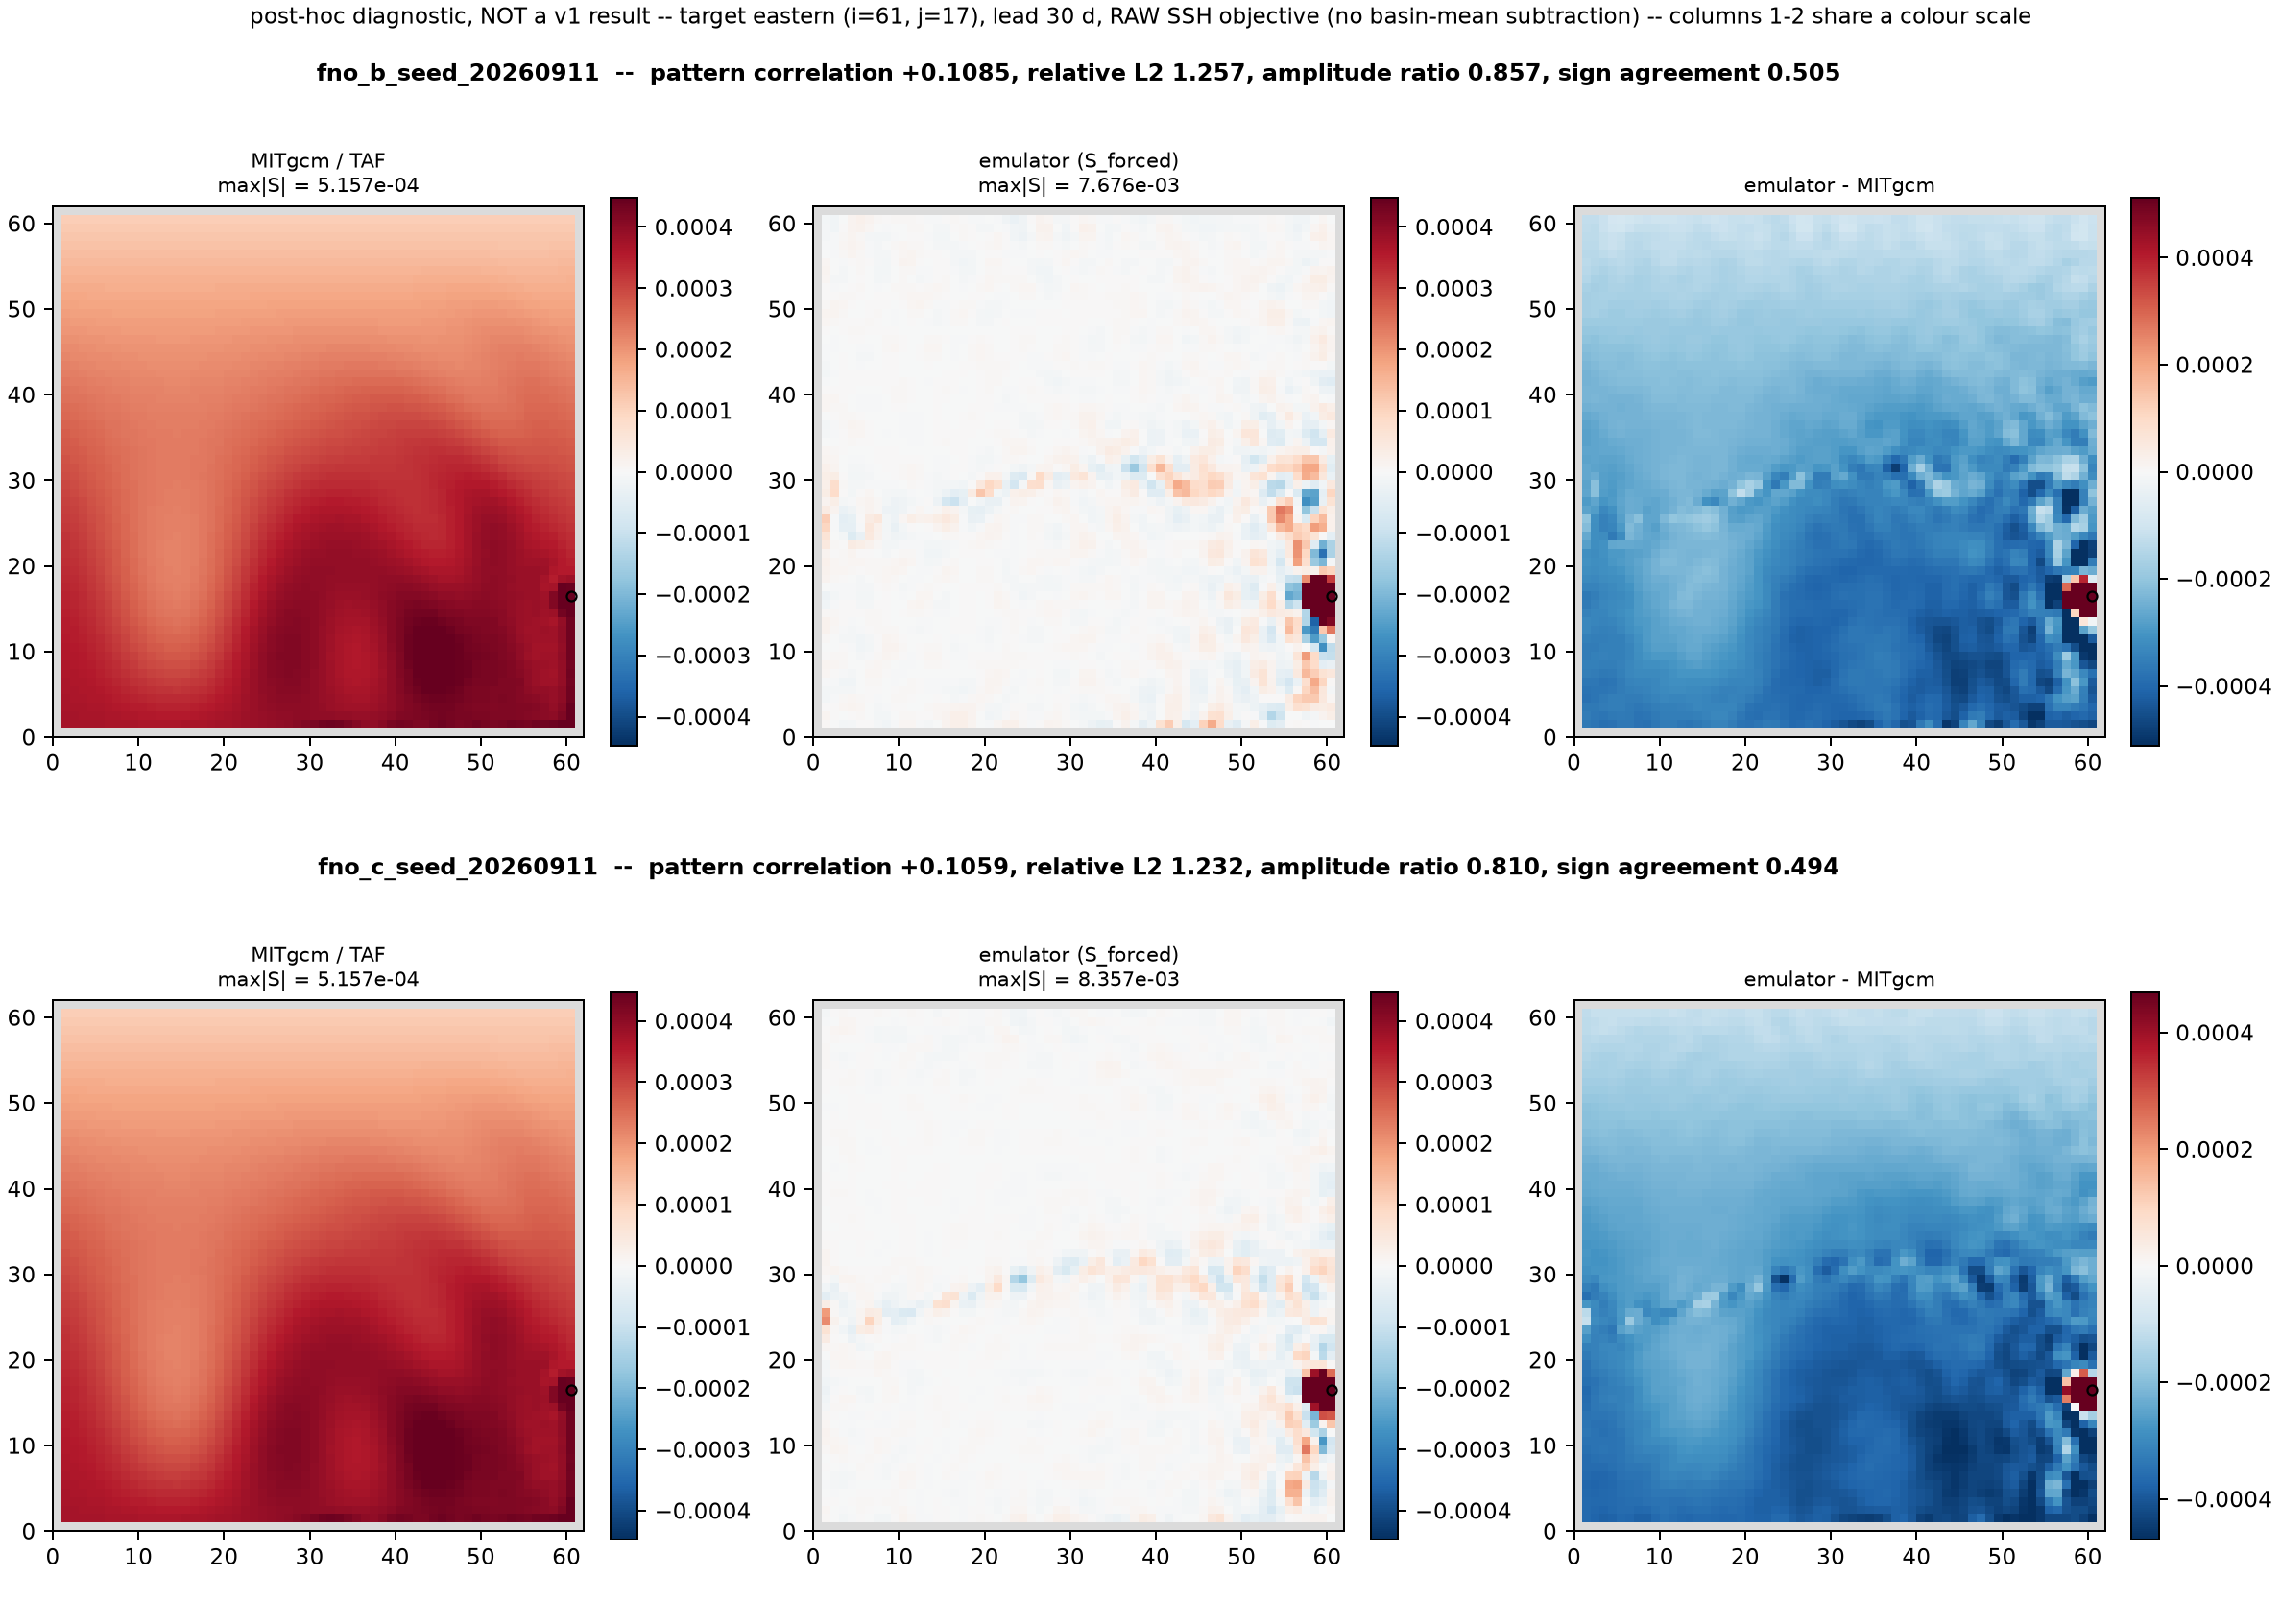
\includegraphics[width=\textwidth]{figures/adj_eastern_raw_ssh_030.png}
\caption{Eastern target, $J_{\mathrm{raw}}$, lead 30~d.}
\label{fig:east_raw030}
\end{figure}

\begin{figure}[htbp]
\centering
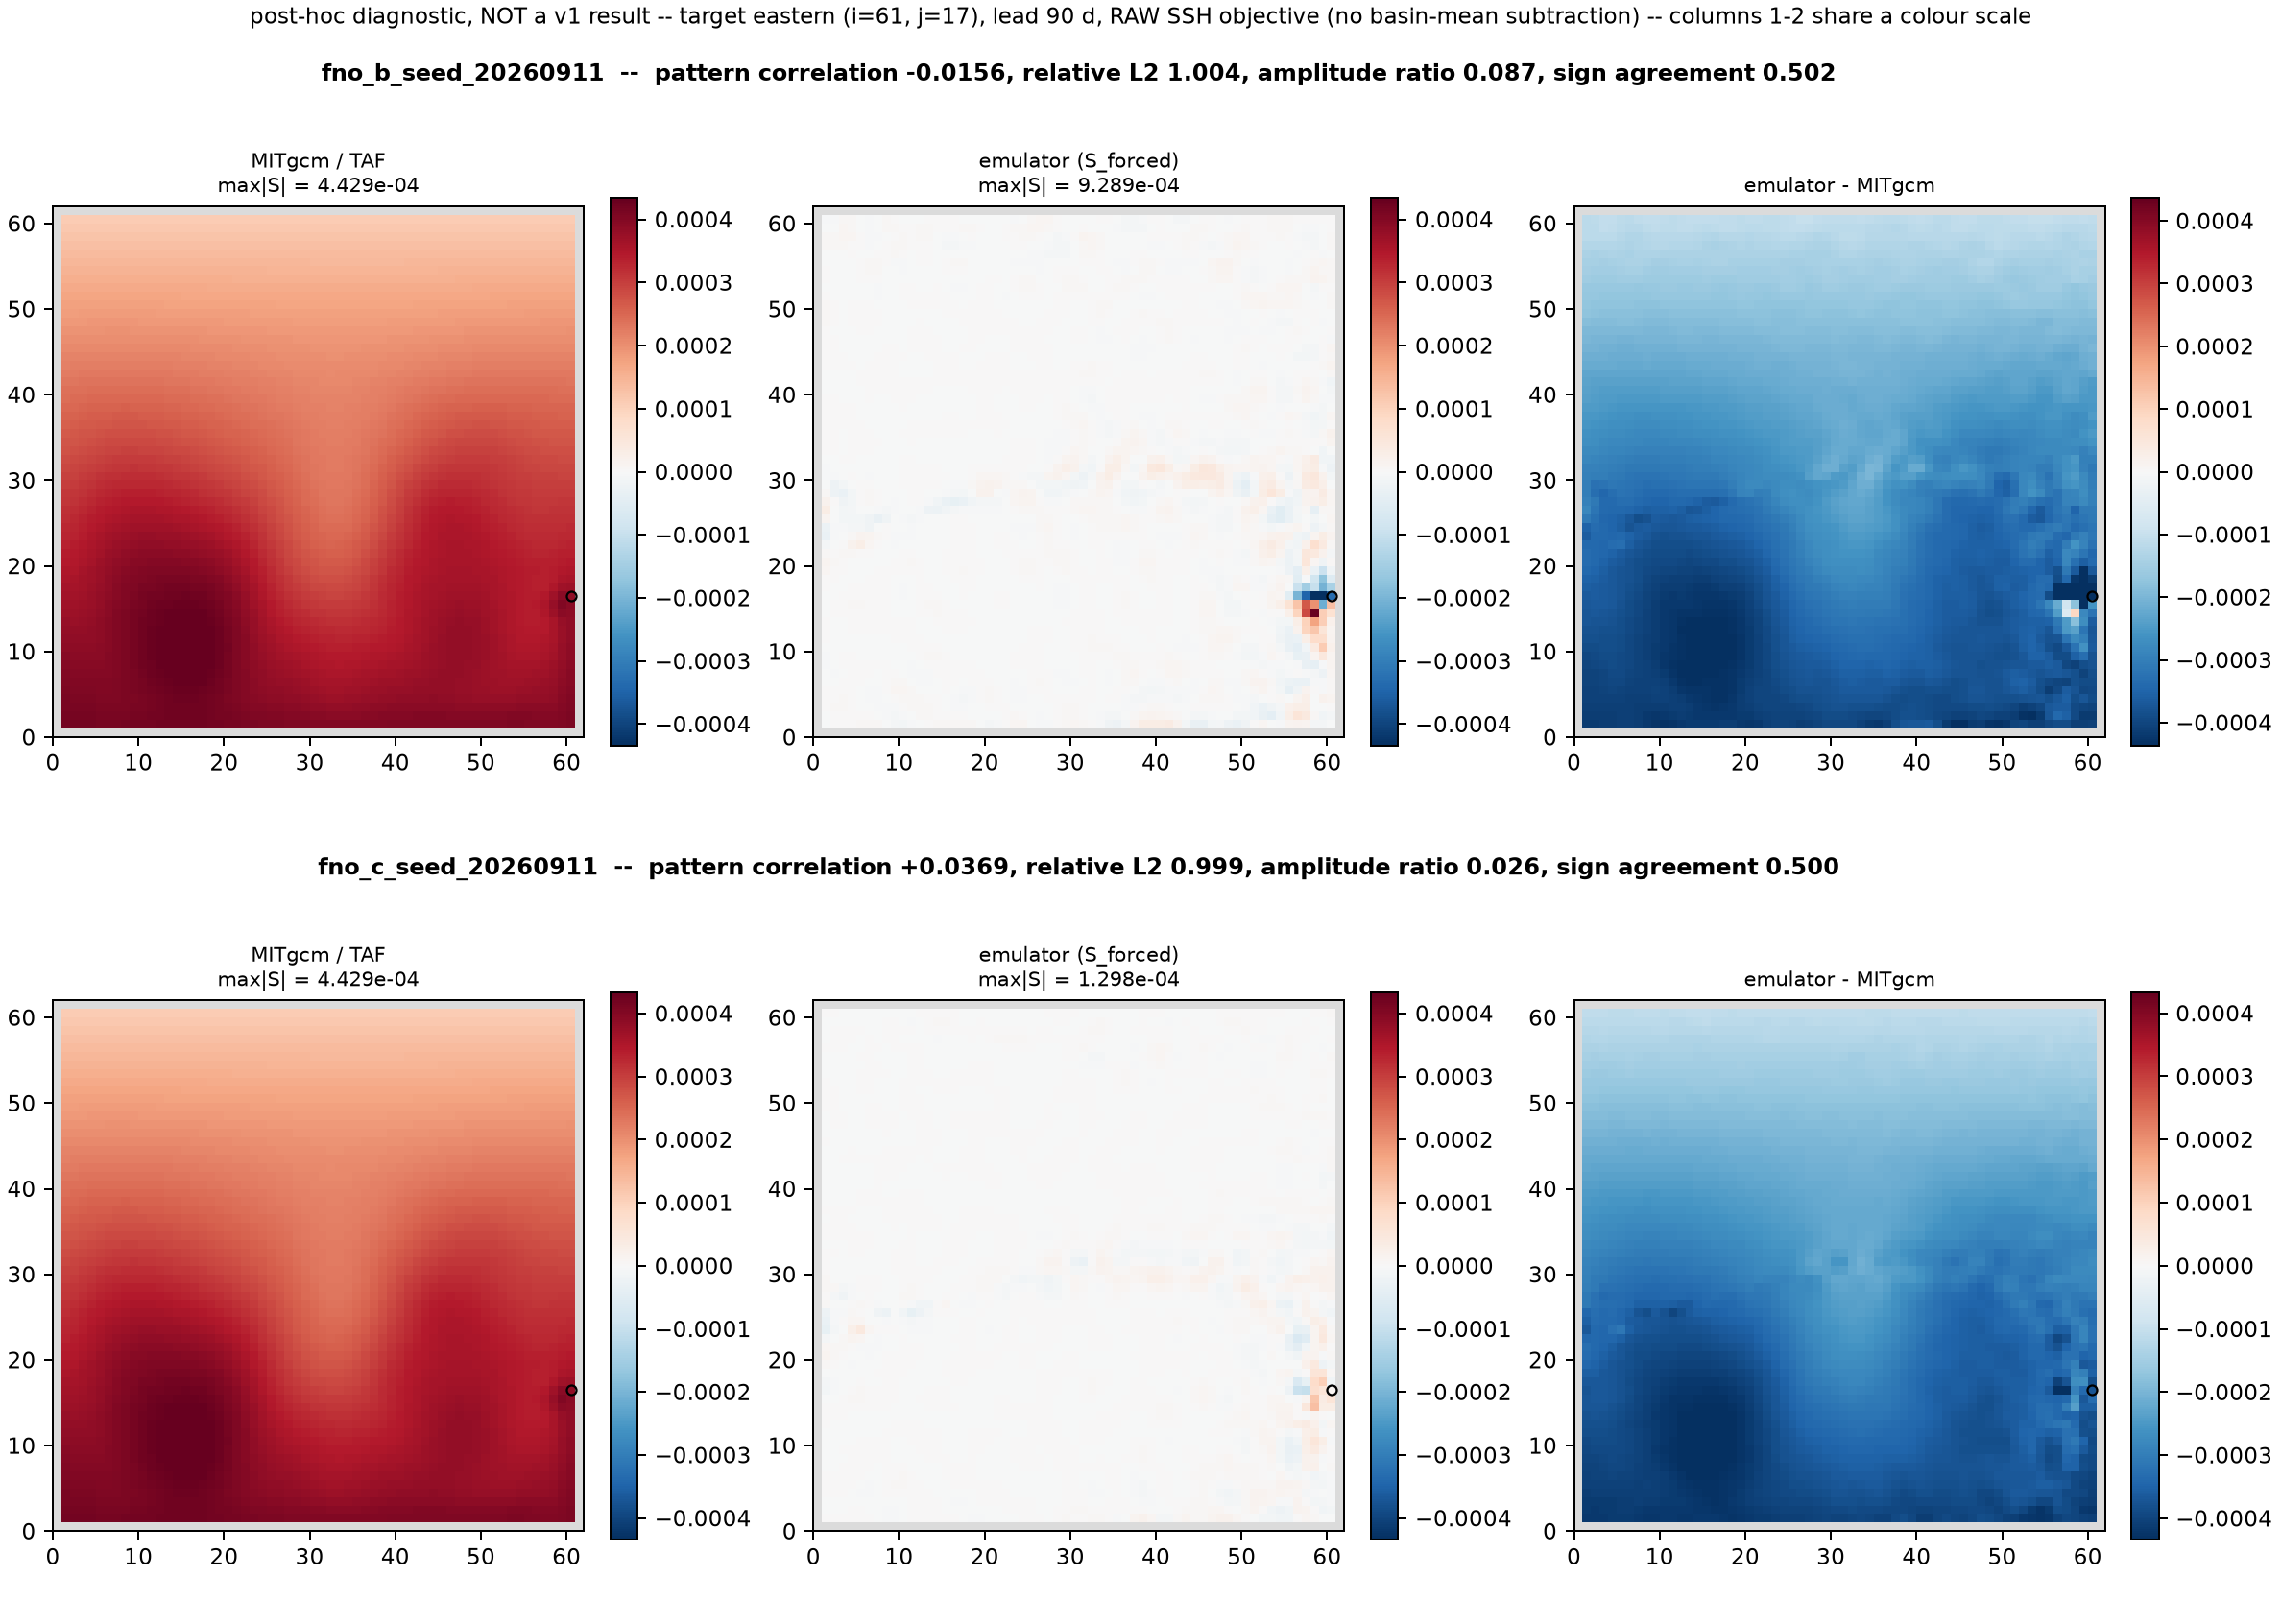
\includegraphics[width=\textwidth]{figures/adj_eastern_raw_ssh_090.png}
\caption{Eastern target, $J_{\mathrm{raw}}$, lead 90~d. Both emulators have
damped the signal to 3--9\% of truth, and $\varepsilon_2\to1$ accordingly.}
\label{fig:east_raw090}
\end{figure}

\begin{figure}[htbp]
\centering
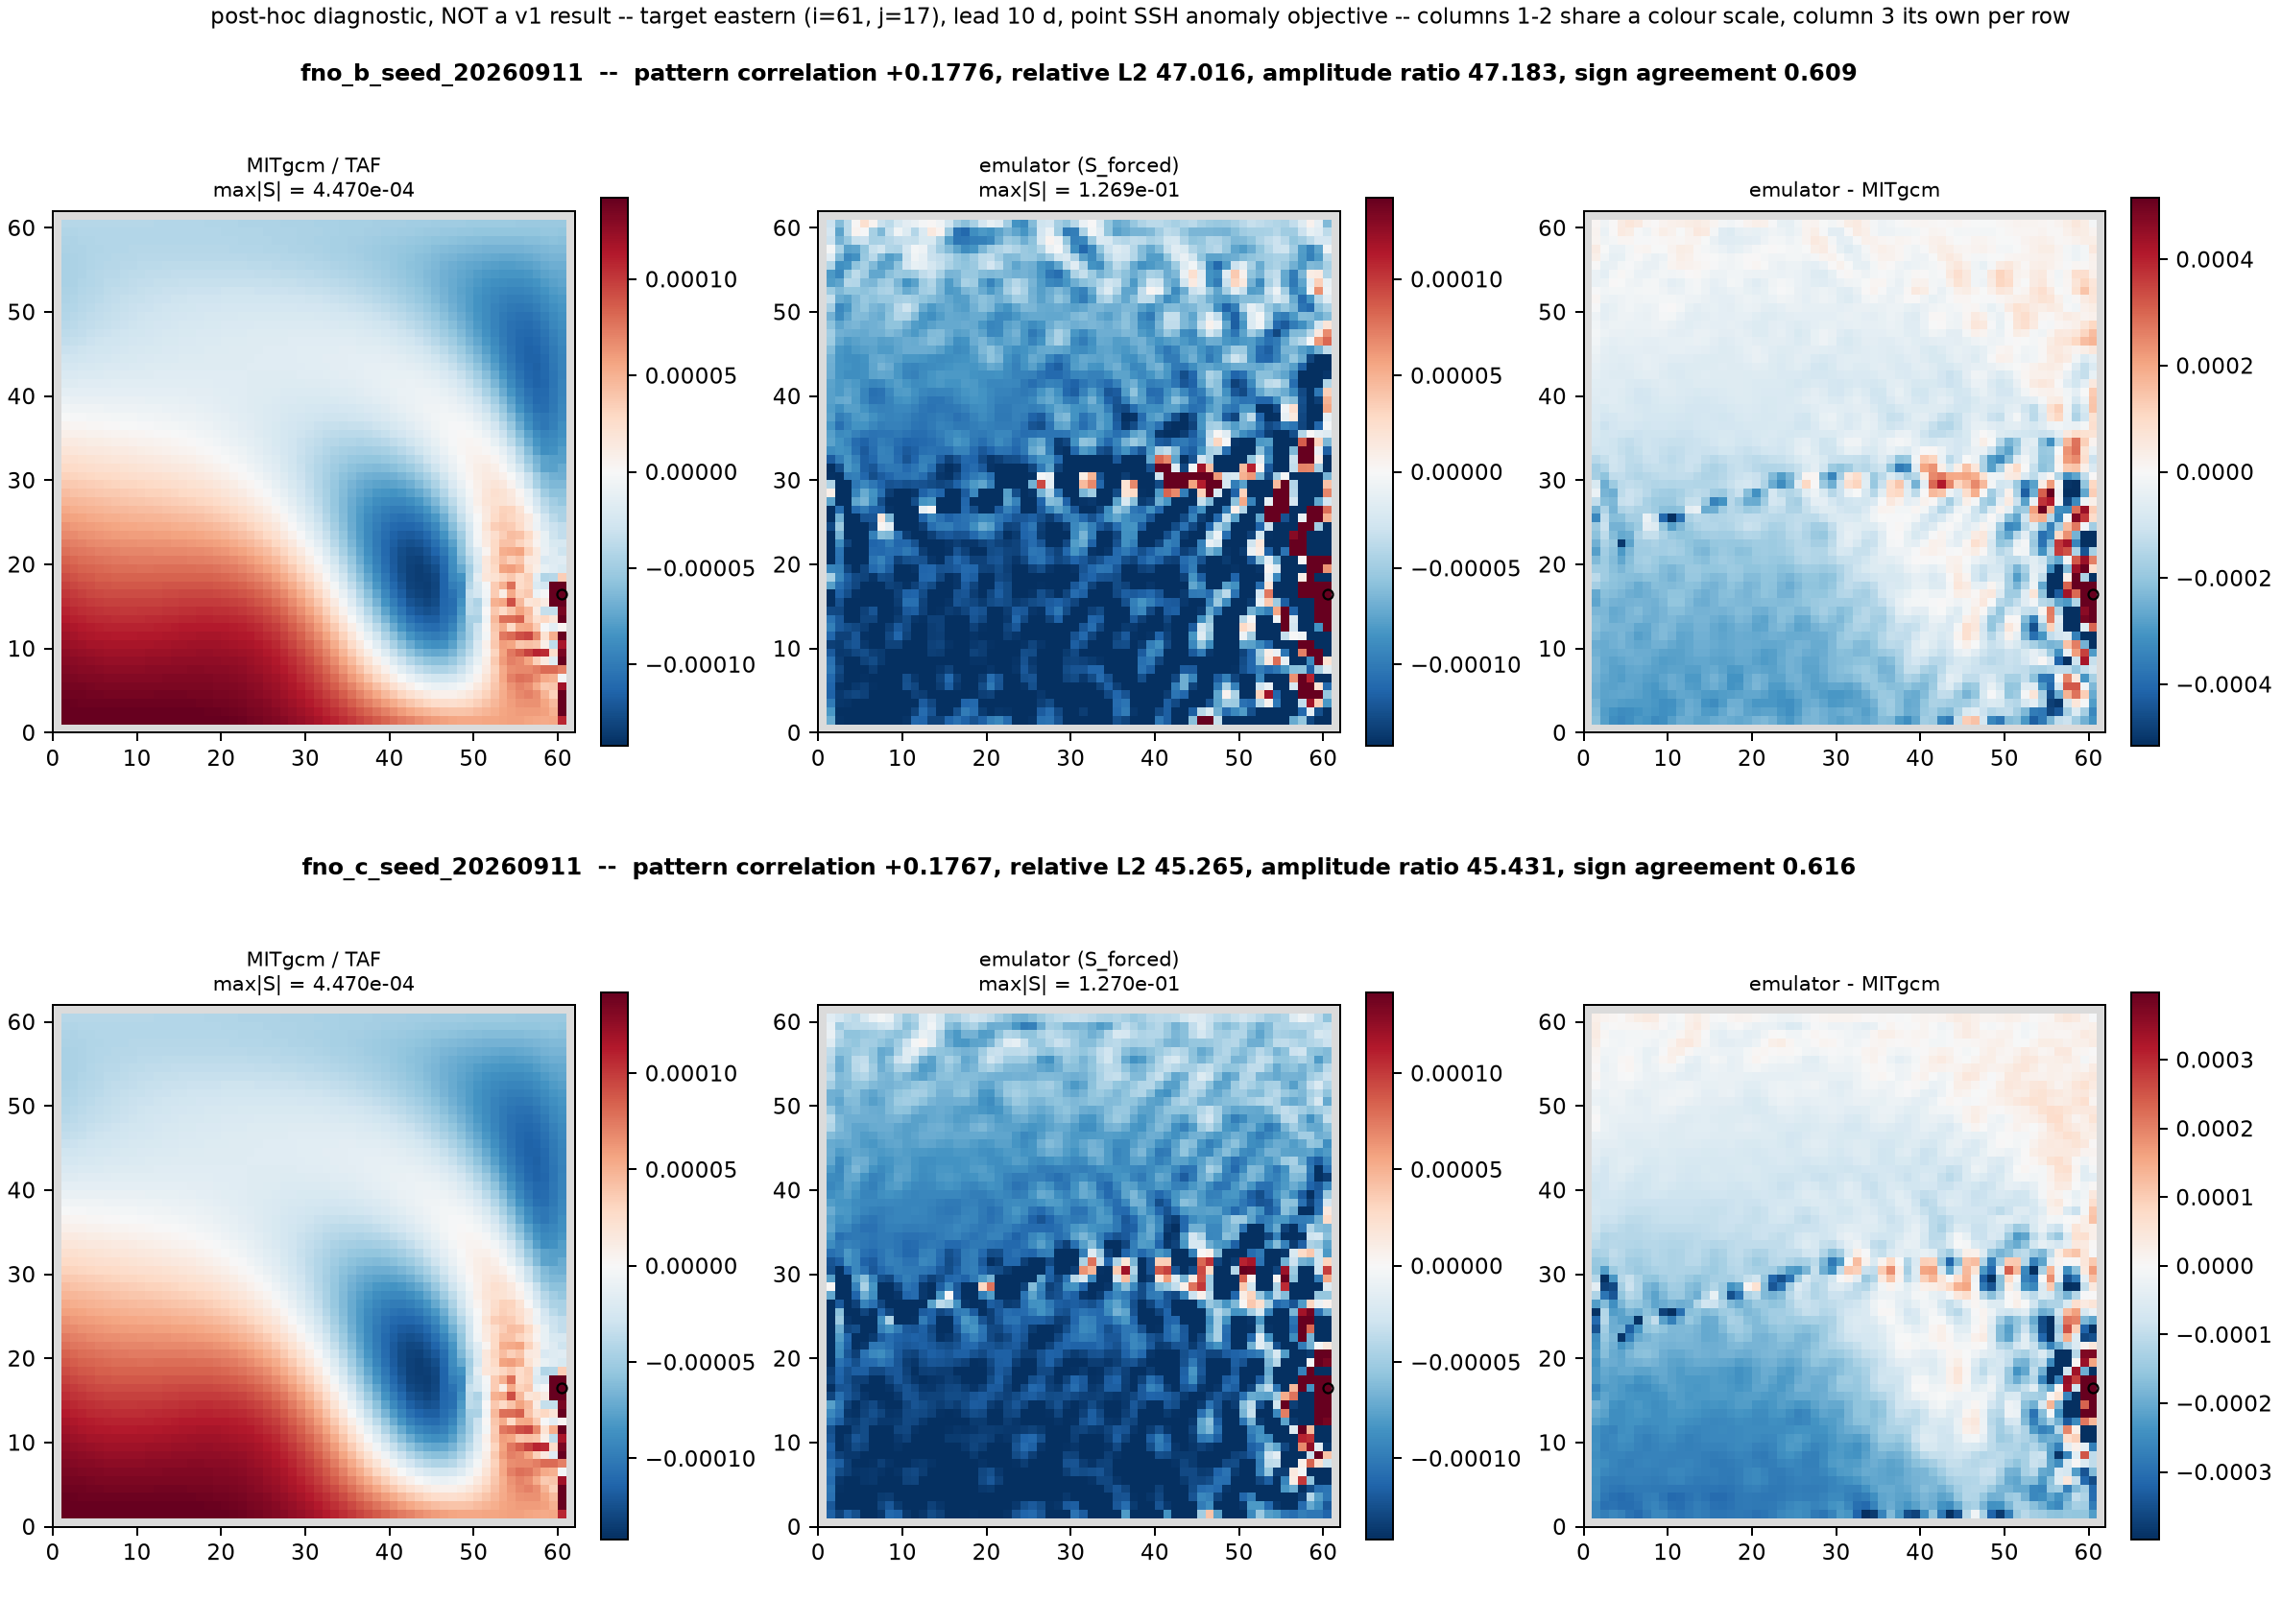
\includegraphics[width=\textwidth]{figures/adj_eastern_ssh_anomaly_010.png}
\caption{Eastern target, $J_{\mathrm{anom}}$, lead 10~d --- the largest
amplitude error in this report ($\alpha\approx47$). The reference is a smooth
large-scale dipole with a small norm; the emulator is dominated by a
boundary-hugging spike and jet-axis speckle.}
\label{fig:east_anom010}
\end{figure}

\begin{figure}[htbp]
\centering
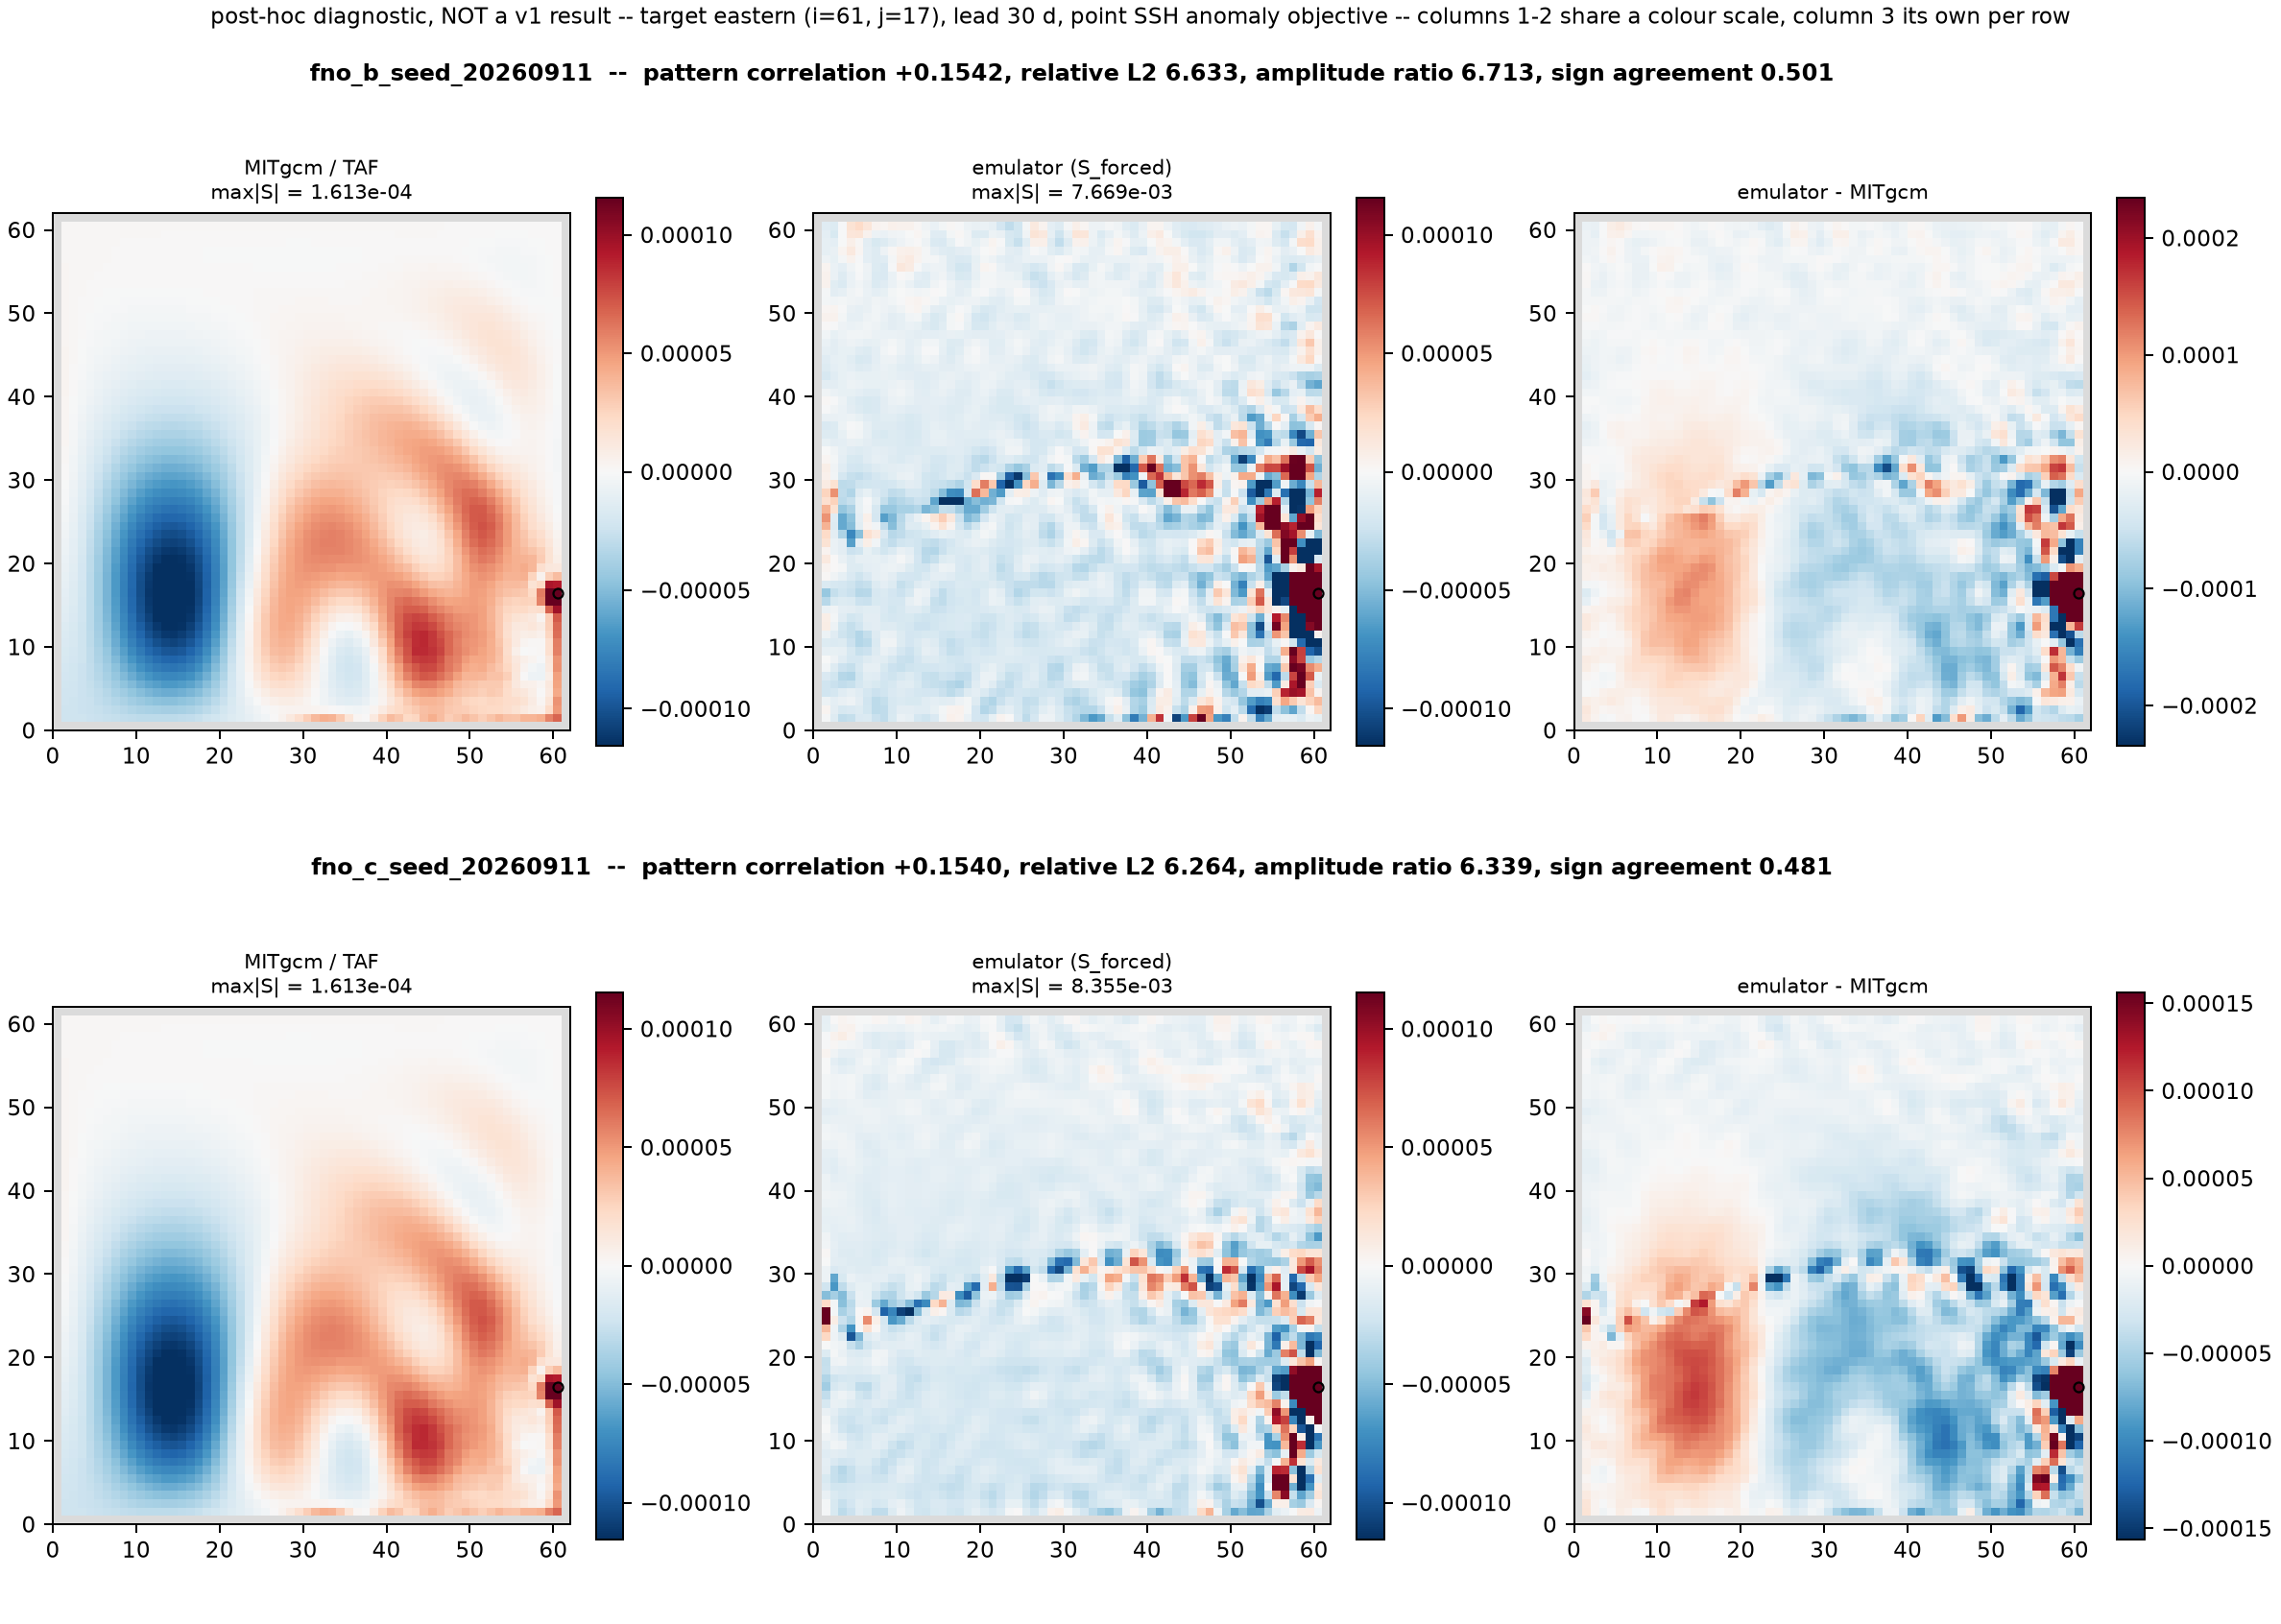
\includegraphics[width=\textwidth]{figures/adj_eastern_ssh_anomaly_030.png}
\caption{Eastern target, $J_{\mathrm{anom}}$, lead 30~d.}
\label{fig:east_anom030}
\end{figure}

\begin{figure}[htbp]
\centering
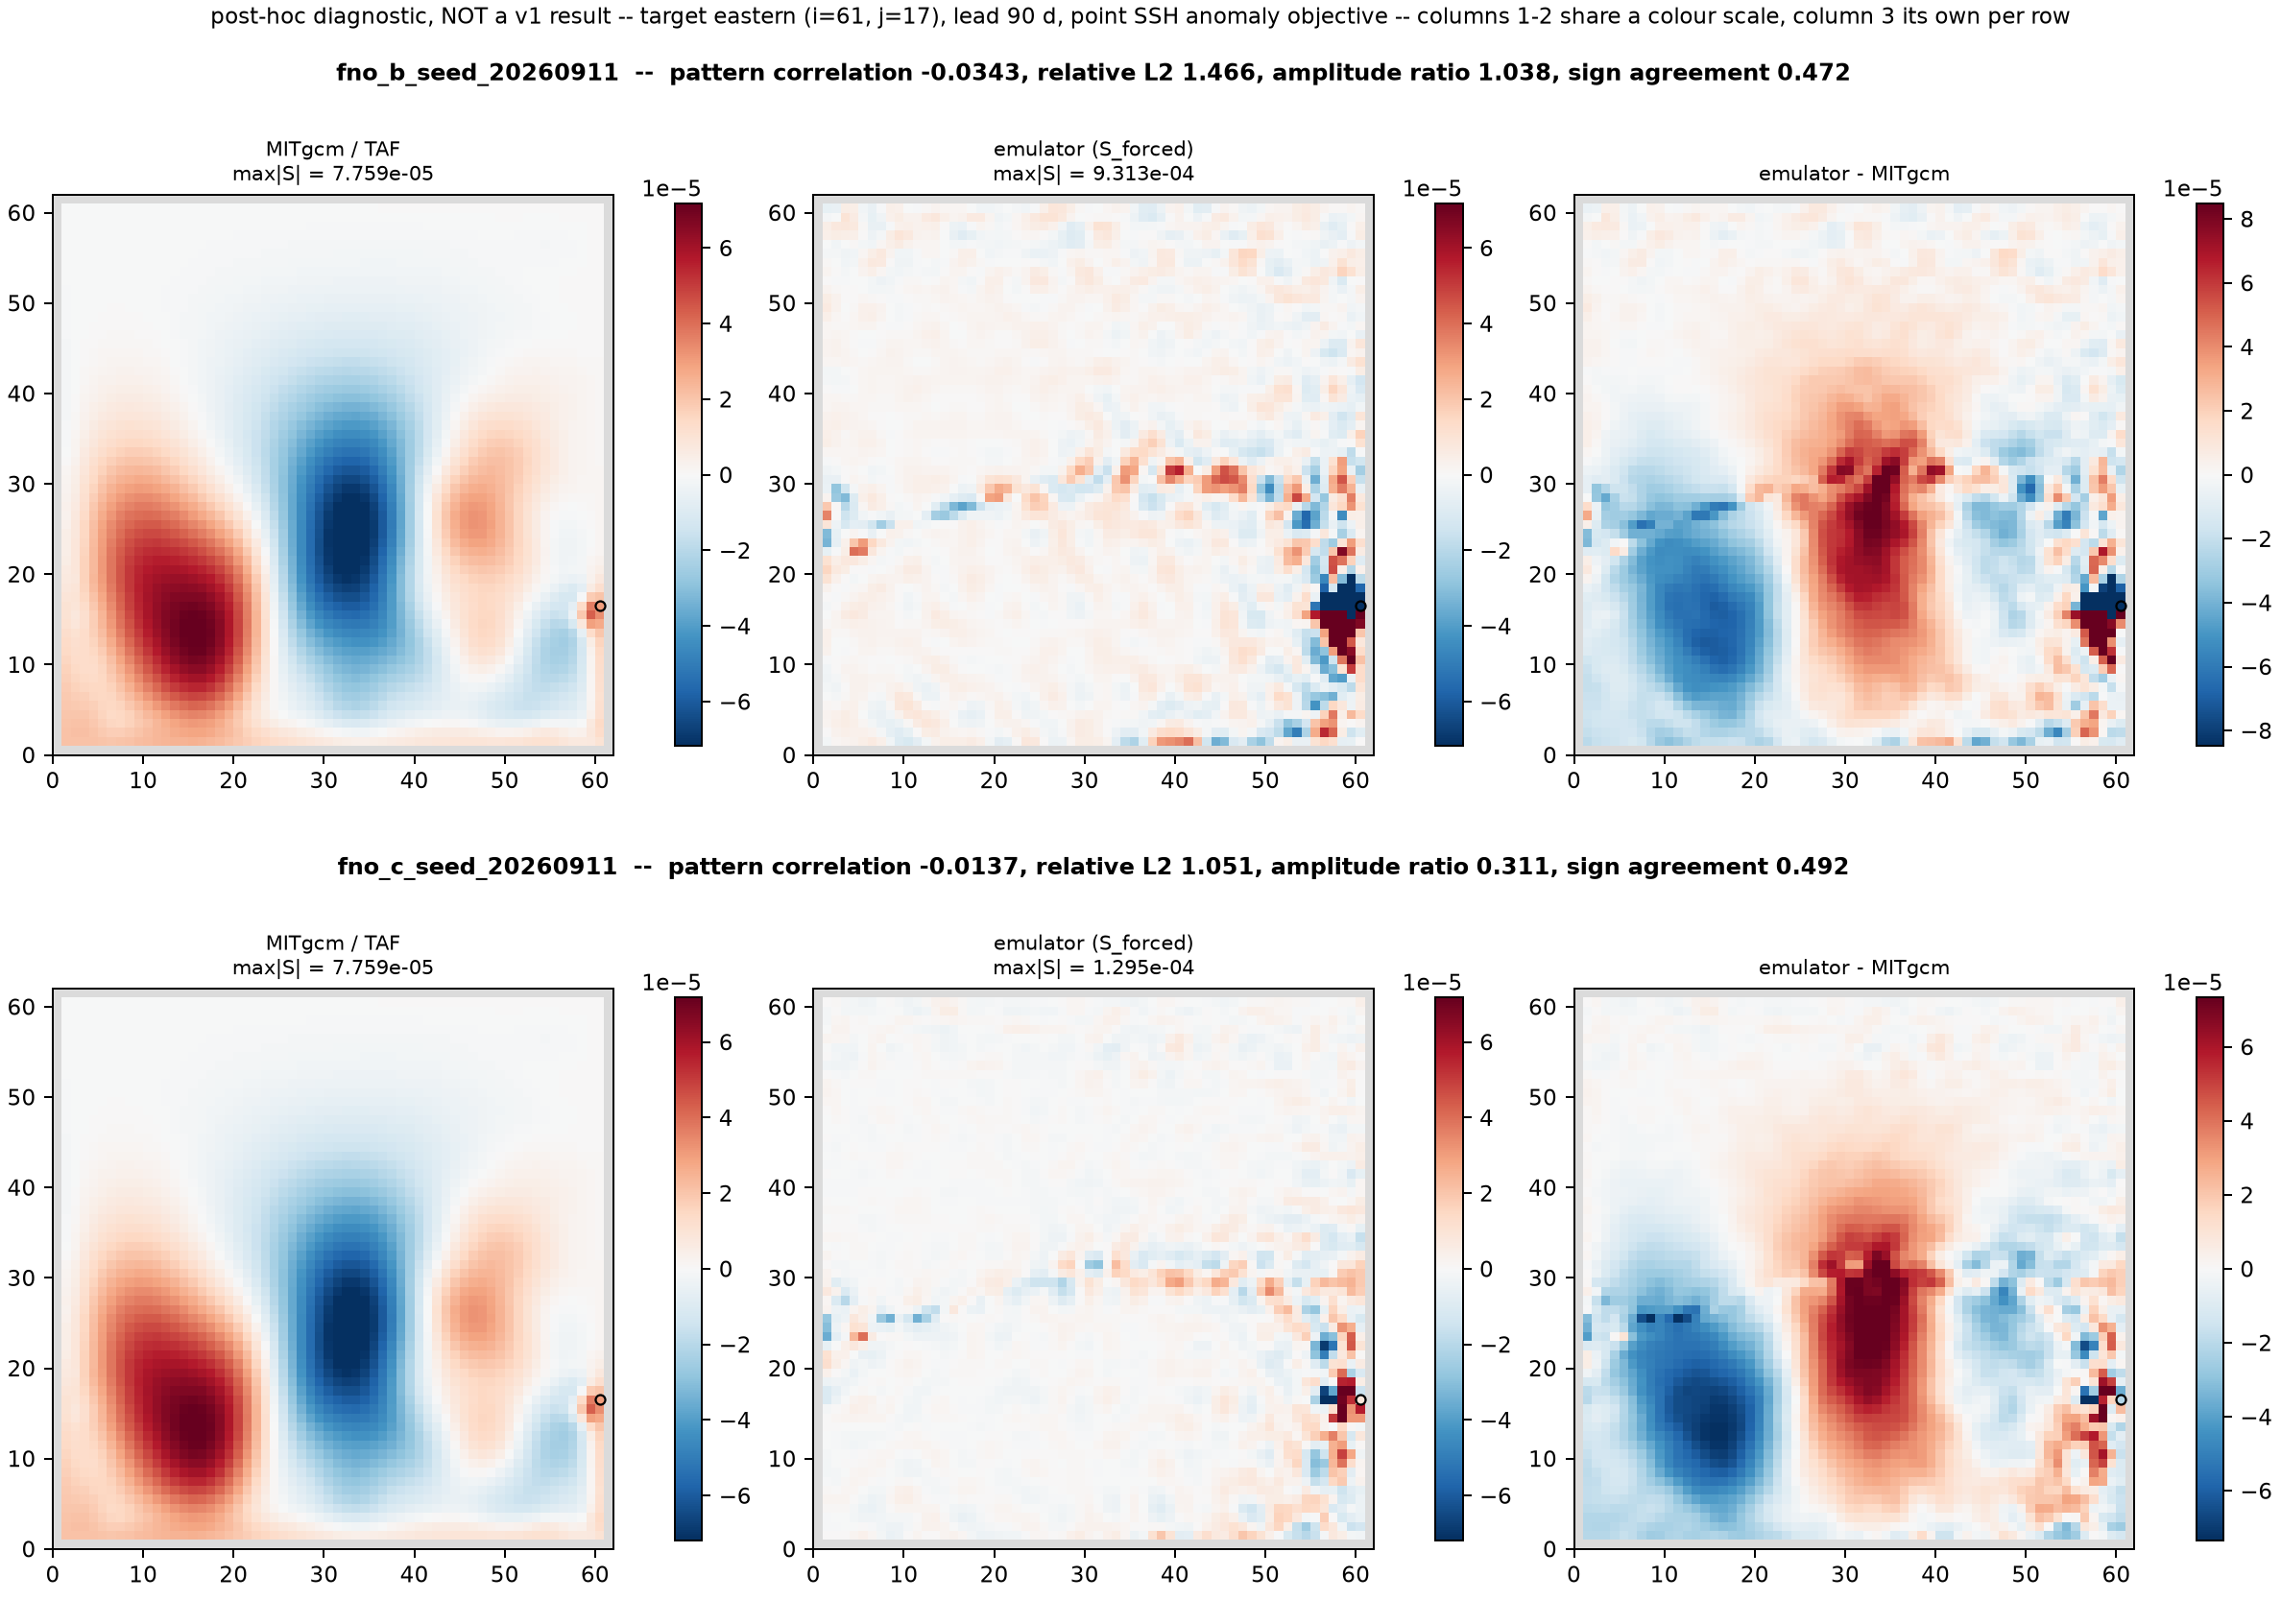
\includegraphics[width=\textwidth]{figures/adj_eastern_ssh_anomaly_090.png}
\caption{Eastern target, $J_{\mathrm{anom}}$, lead 90~d. The control's amplitude
is almost exactly right ($\alpha=1.04$) with correlation $-0.03$: the right
amount of sensitivity in the wrong places. The response arm lowers the error by
having less sensitivity, not by relocating it.}
\label{fig:east_anom090}
\end{figure}

\subsubsection{Western target}
\label{sec:western}

The western target is $p^\star=(2,17)$, the second wet column, inside the western
boundary current. This is the study's pre-declared confirmatory target, chosen
because boundary-current sensitivity is what an ocean adjoint is normally used
for and what a spectral emulator should find hardest.

\begin{table}[H]
\centering
\small
\begin{tabular}{llrrrrrr}
\toprule
& & \multicolumn{3}{c}{Control} & \multicolumn{3}{c}{Response} \\
\cmidrule(lr){3-5}\cmidrule(lr){6-8}
Objective & Lead (d) & $\rho$ & $\varepsilon_2$ & $\alpha$ & $\rho$ & $\varepsilon_2$ & $\alpha$ \\
\midrule
$J_{\mathrm{raw}}$  & 10 & $+0.064$ & 9.936 & 9.912 & $+0.071$ & \textbf{8.814} & 8.794 \\
$J_{\mathrm{raw}}$  & 30 & $+0.015$ & 1.563 & 1.224 & $+0.029$ & \textbf{1.280} & 0.827 \\
$J_{\mathrm{raw}}$  & 90 & $-0.022$ & 1.179 & 0.606 & $-0.023$ & \textbf{1.115} & 0.455 \\
$J_{\mathrm{anom}}$ & 10 & $+0.051$ & 40.854 & 40.892 & $+0.055$ & \textbf{36.222} & 36.263 \\
$J_{\mathrm{anom}}$ & 30 & $+0.009$ & 9.579 & 9.536 & $+0.027$ & \textbf{6.500} & 6.450 \\
$J_{\mathrm{anom}}$ & 90 & $-0.030$ & 7.063 & 6.962 & $-0.024$ & \textbf{5.371} & 5.254 \\
\bottomrule
\end{tabular}
\caption{Western target $(2,17)$, the confirmatory target. The response arm's
reductions in relative $L_2$ are the largest of the three targets under
$J_{\mathrm{anom}}$: 11\%, 32\% and 24\% at leads 10, 30 and 90.}
\label{tab:western}
\end{table}

\paragraph{Discussion} The western target is where the failure is most visually
stark. Under $J_{\mathrm{anom}}$ at lead 10 (Figure~\ref{fig:west_anom010}) the
reference is smooth and organized: a positive tongue extending east from the
boundary near $j\approx20$, a deep negative pool centred near $(46,10)$, positive
lobes on the northern rim and in the north-east, and a narrow band of
fine structure in the first few columns at the target itself --- the boundary
current's own signature. The emulator's map, on the same colour scale, is
saturated grid-scale noise across the entire basin, with alternating cells at
$\pm$ the full scale. Its peak value is $1.47\times10^{-1}$ against
$3.2\times10^{-4}$ for truth: a factor of 460 at the peak, 41 in $L_2$.
At lead 90 (Figure~\ref{fig:west_anom090}) the reference has organized itself
into a clean pair of meridionally elongated lobes --- exactly the westward Rossby
signal an ocean adjoint should show --- while the emulator has become a
diagonal-striped checkerboard, still 7$\times$ too large. This is the single
clearest statement in the study that the emulator's Jacobian is dominated by
high-wavenumber content that the true Jacobian does not contain.

Under $J_{\mathrm{raw}}$ (Figures~\ref{fig:west_raw010}--\ref{fig:west_raw090})
the reference at lead 10 is almost uniformly positive: because the basin mean is
exactly conserved, any perturbation anywhere raises the raw target value by
roughly its share of that conserved total, on top of the local boundary
structure. This is precisely the trivial signal that $J_{\mathrm{anom}}$'s mean
subtraction was designed to remove, and comparing the two objectives at the same
target and lead shows how much of the raw signal it accounts for: the amplitude
ratio drops from 41 to 9.9 when the pedestal is left in, because the pedestal
inflates the reference norm by roughly a factor of four while leaving the
emulator's grid-scale error unchanged.

The response arm's gains are largest here --- 32\% at lead 30, 24\% at lead 90,
under the confirmatory objective --- and it is the only target where the
amplitude ratio crosses from above 1 to below 1 under $J_{\mathrm{raw}}$
(1.22 to 0.83 at lead 30). Yet the pattern correlation moves from $+0.009$ to
$+0.027$ at lead 30 and stays negative at lead 90. The response term is
demonstrably doing something real and in a consistent direction; what it is
doing is calibrating magnitude, not structure.

\begin{figure}[htbp]
\centering
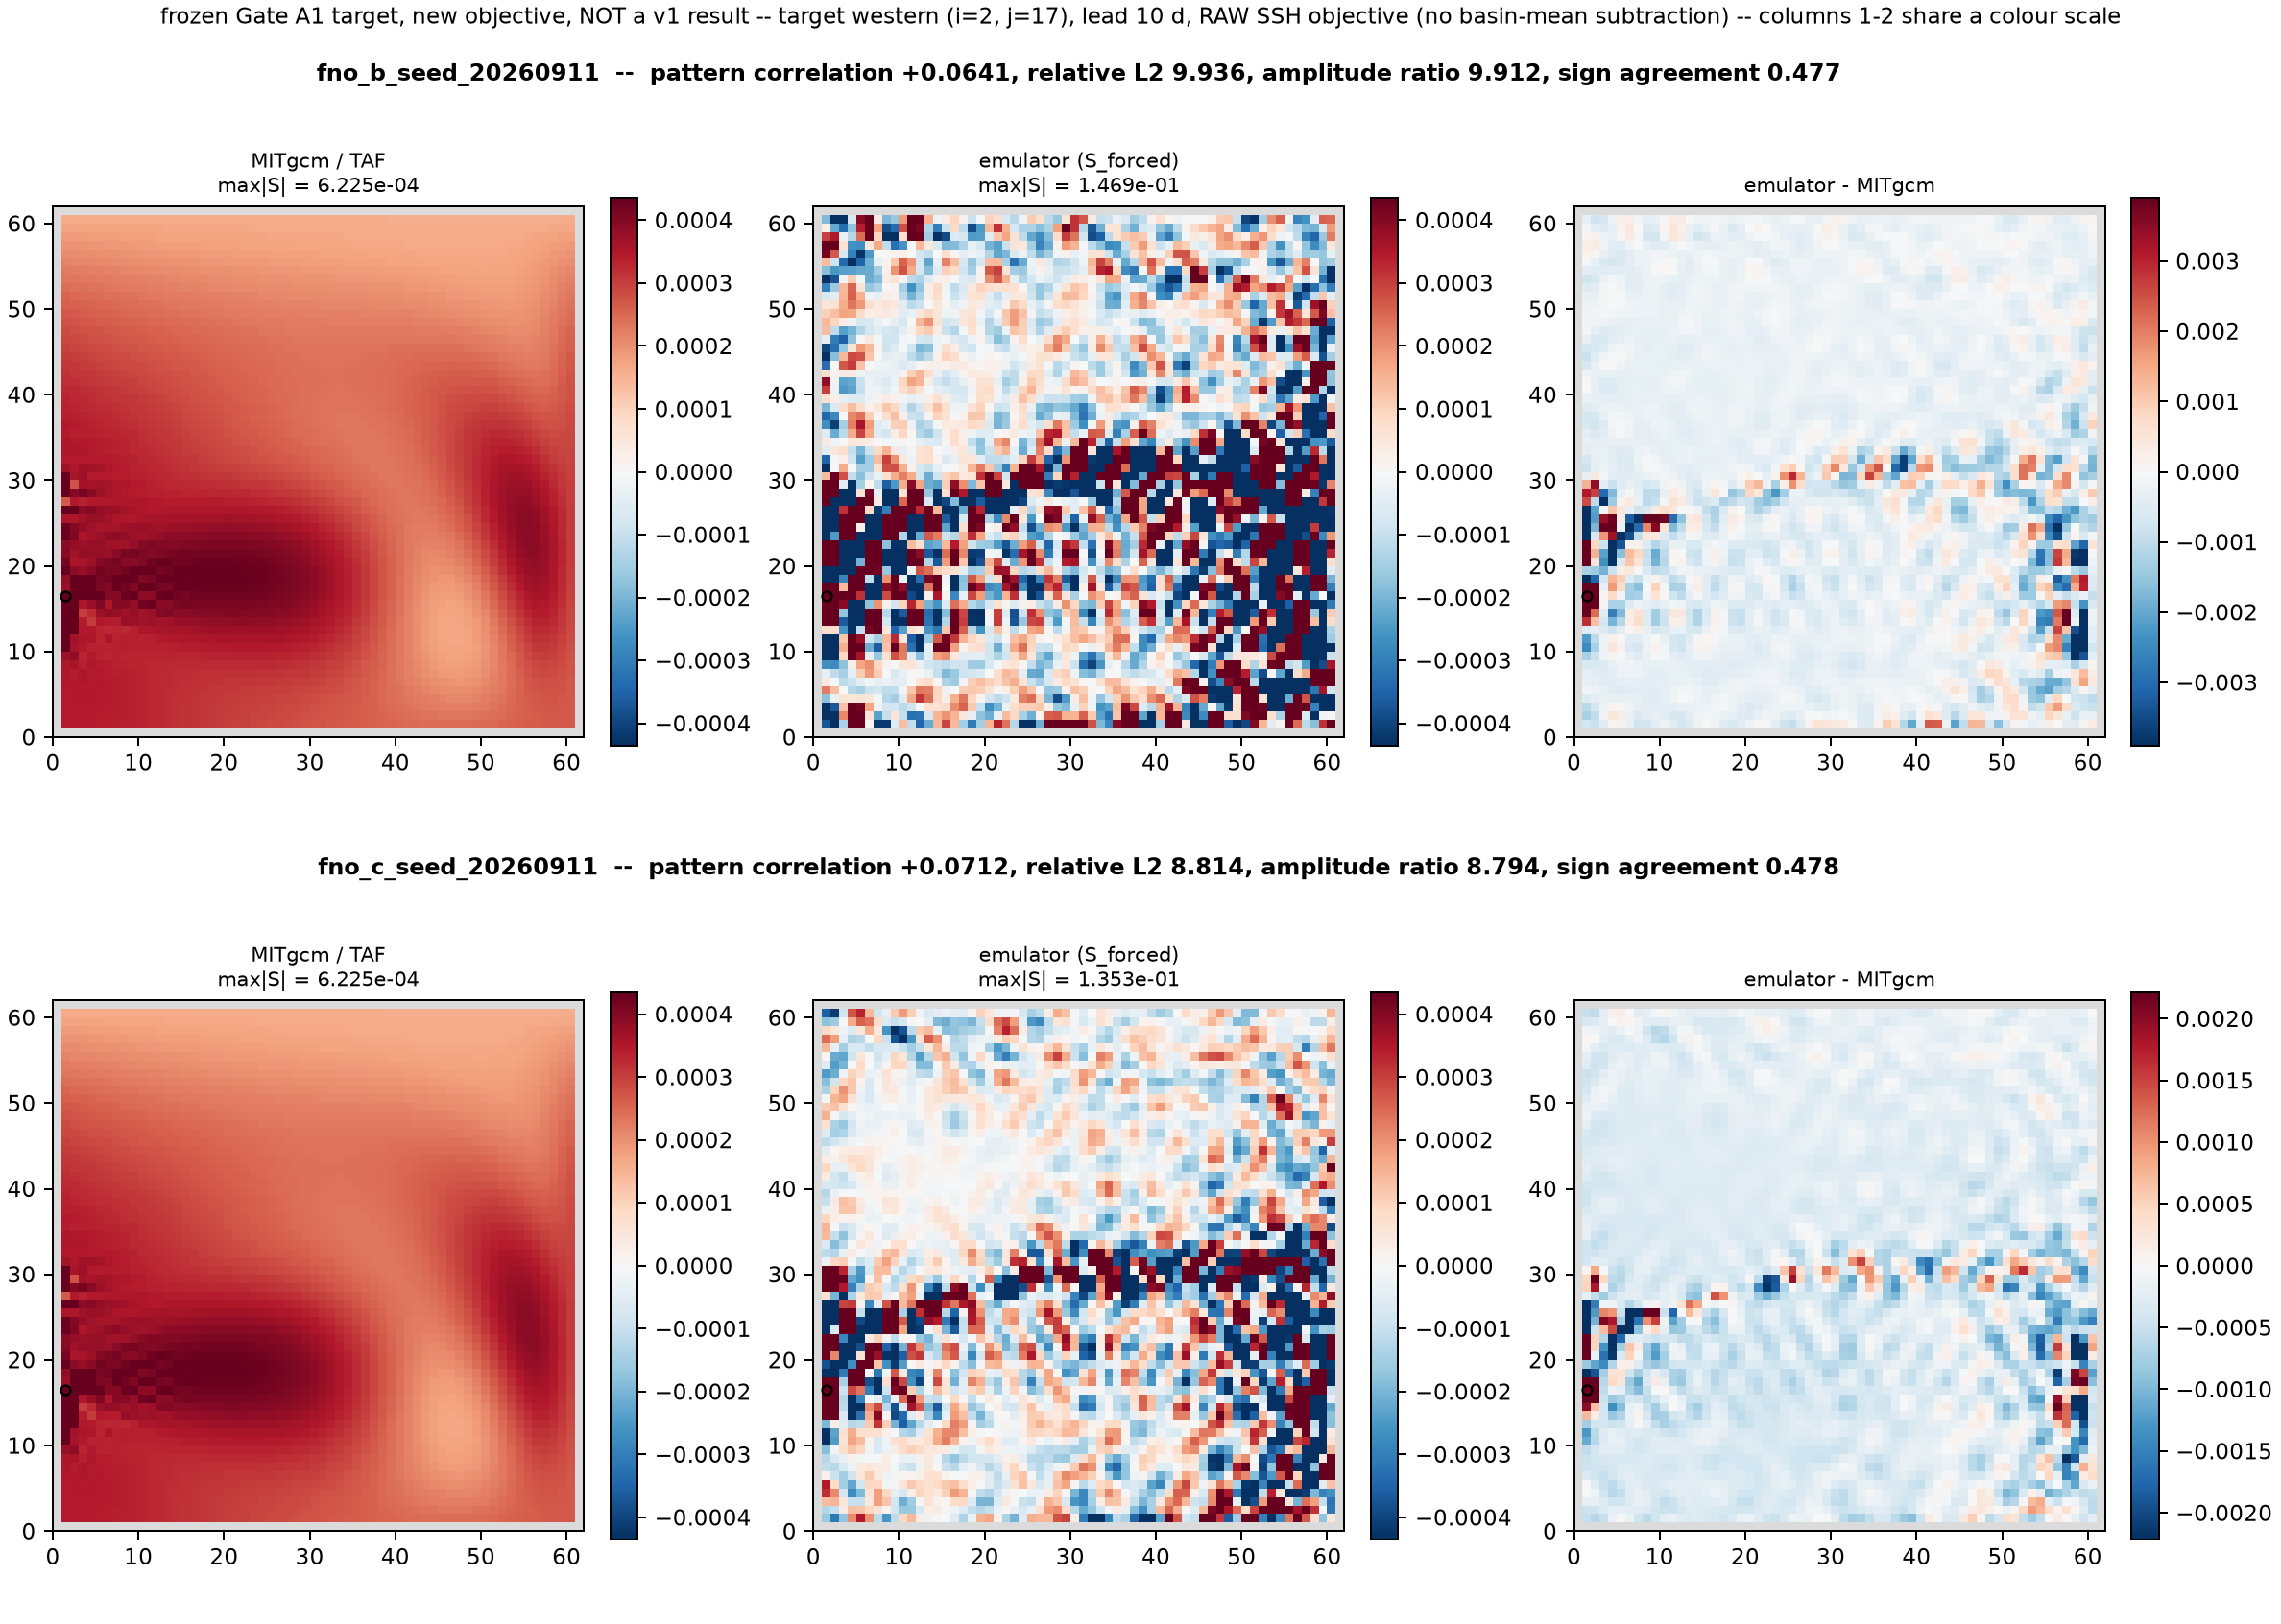
\includegraphics[width=\textwidth]{figures/adj_western_raw_ssh_010.png}
\caption{Western target, $J_{\mathrm{raw}}$, lead 10~d. The reference is almost
uniformly positive --- the exactly conserved basin-mean pedestal plus local
boundary structure --- which is what the anomaly objective's mean subtraction
removes.}
\label{fig:west_raw010}
\end{figure}

\begin{figure}[htbp]
\centering
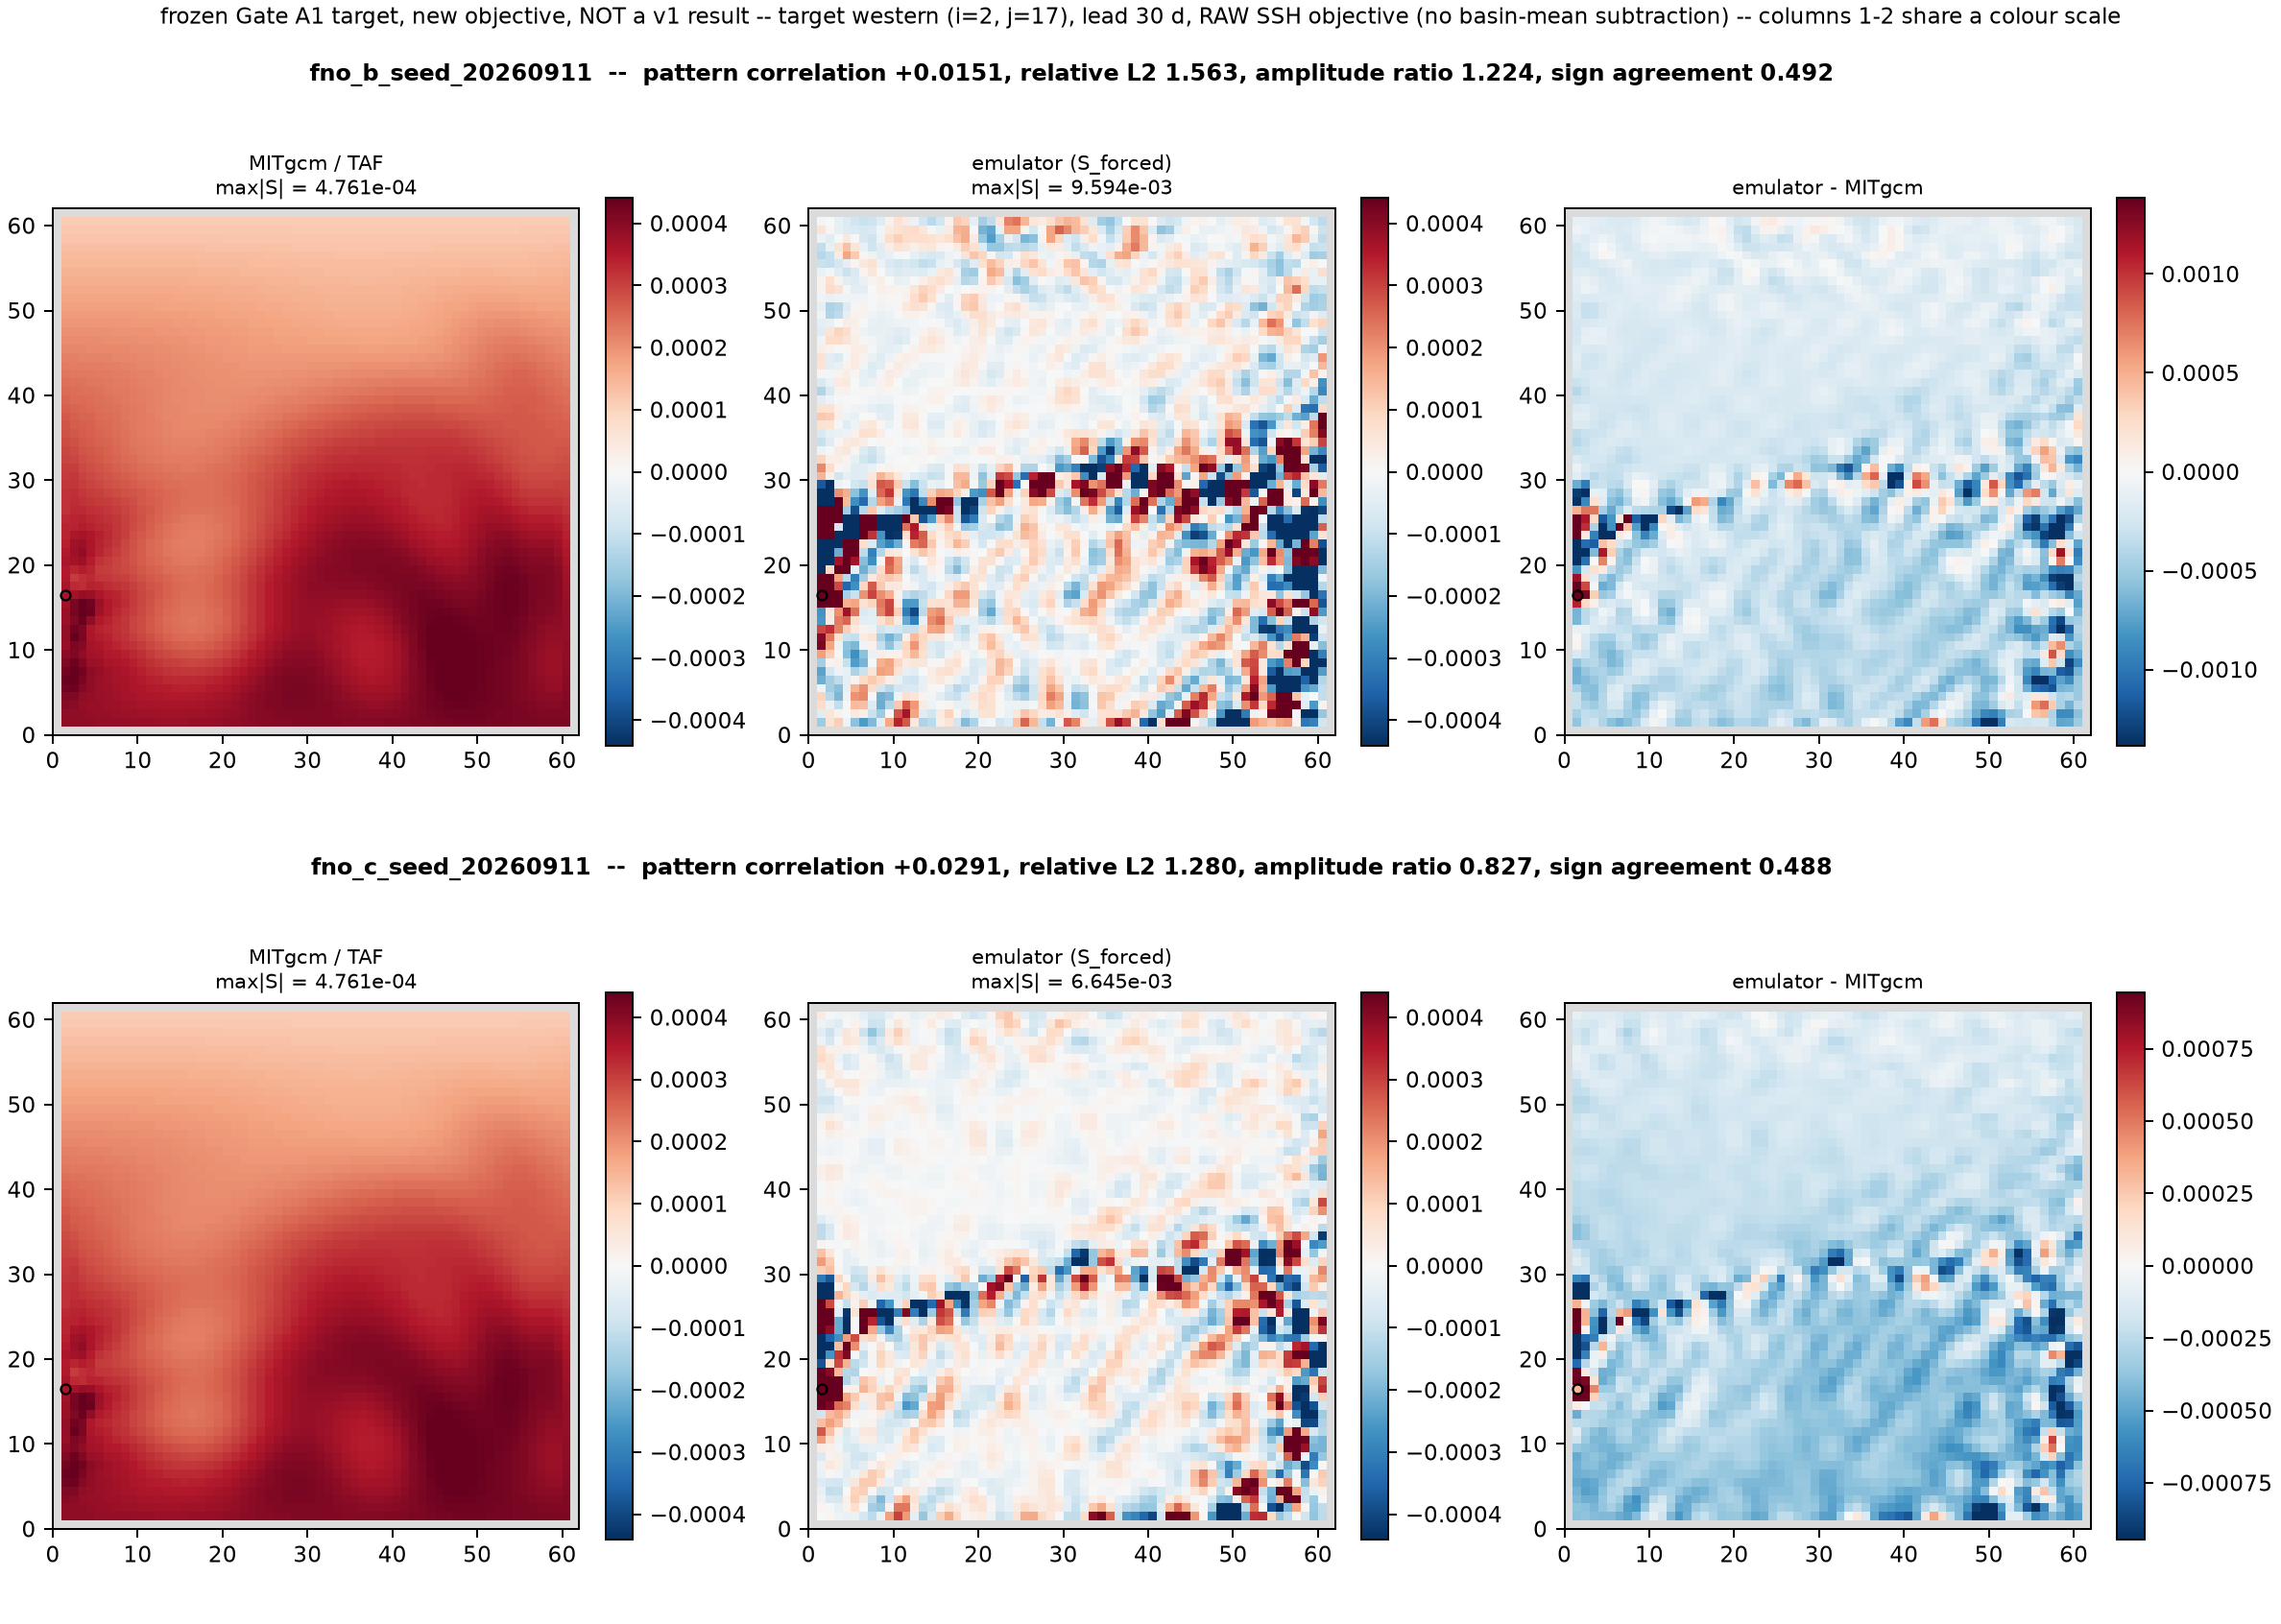
\includegraphics[width=\textwidth]{figures/adj_western_raw_ssh_030.png}
\caption{Western target, $J_{\mathrm{raw}}$, lead 30~d. The only cell in this
report where the response arm's amplitude ratio crosses from above to below 1
(1.22 $\to$ 0.83).}
\label{fig:west_raw030}
\end{figure}

\begin{figure}[htbp]
\centering
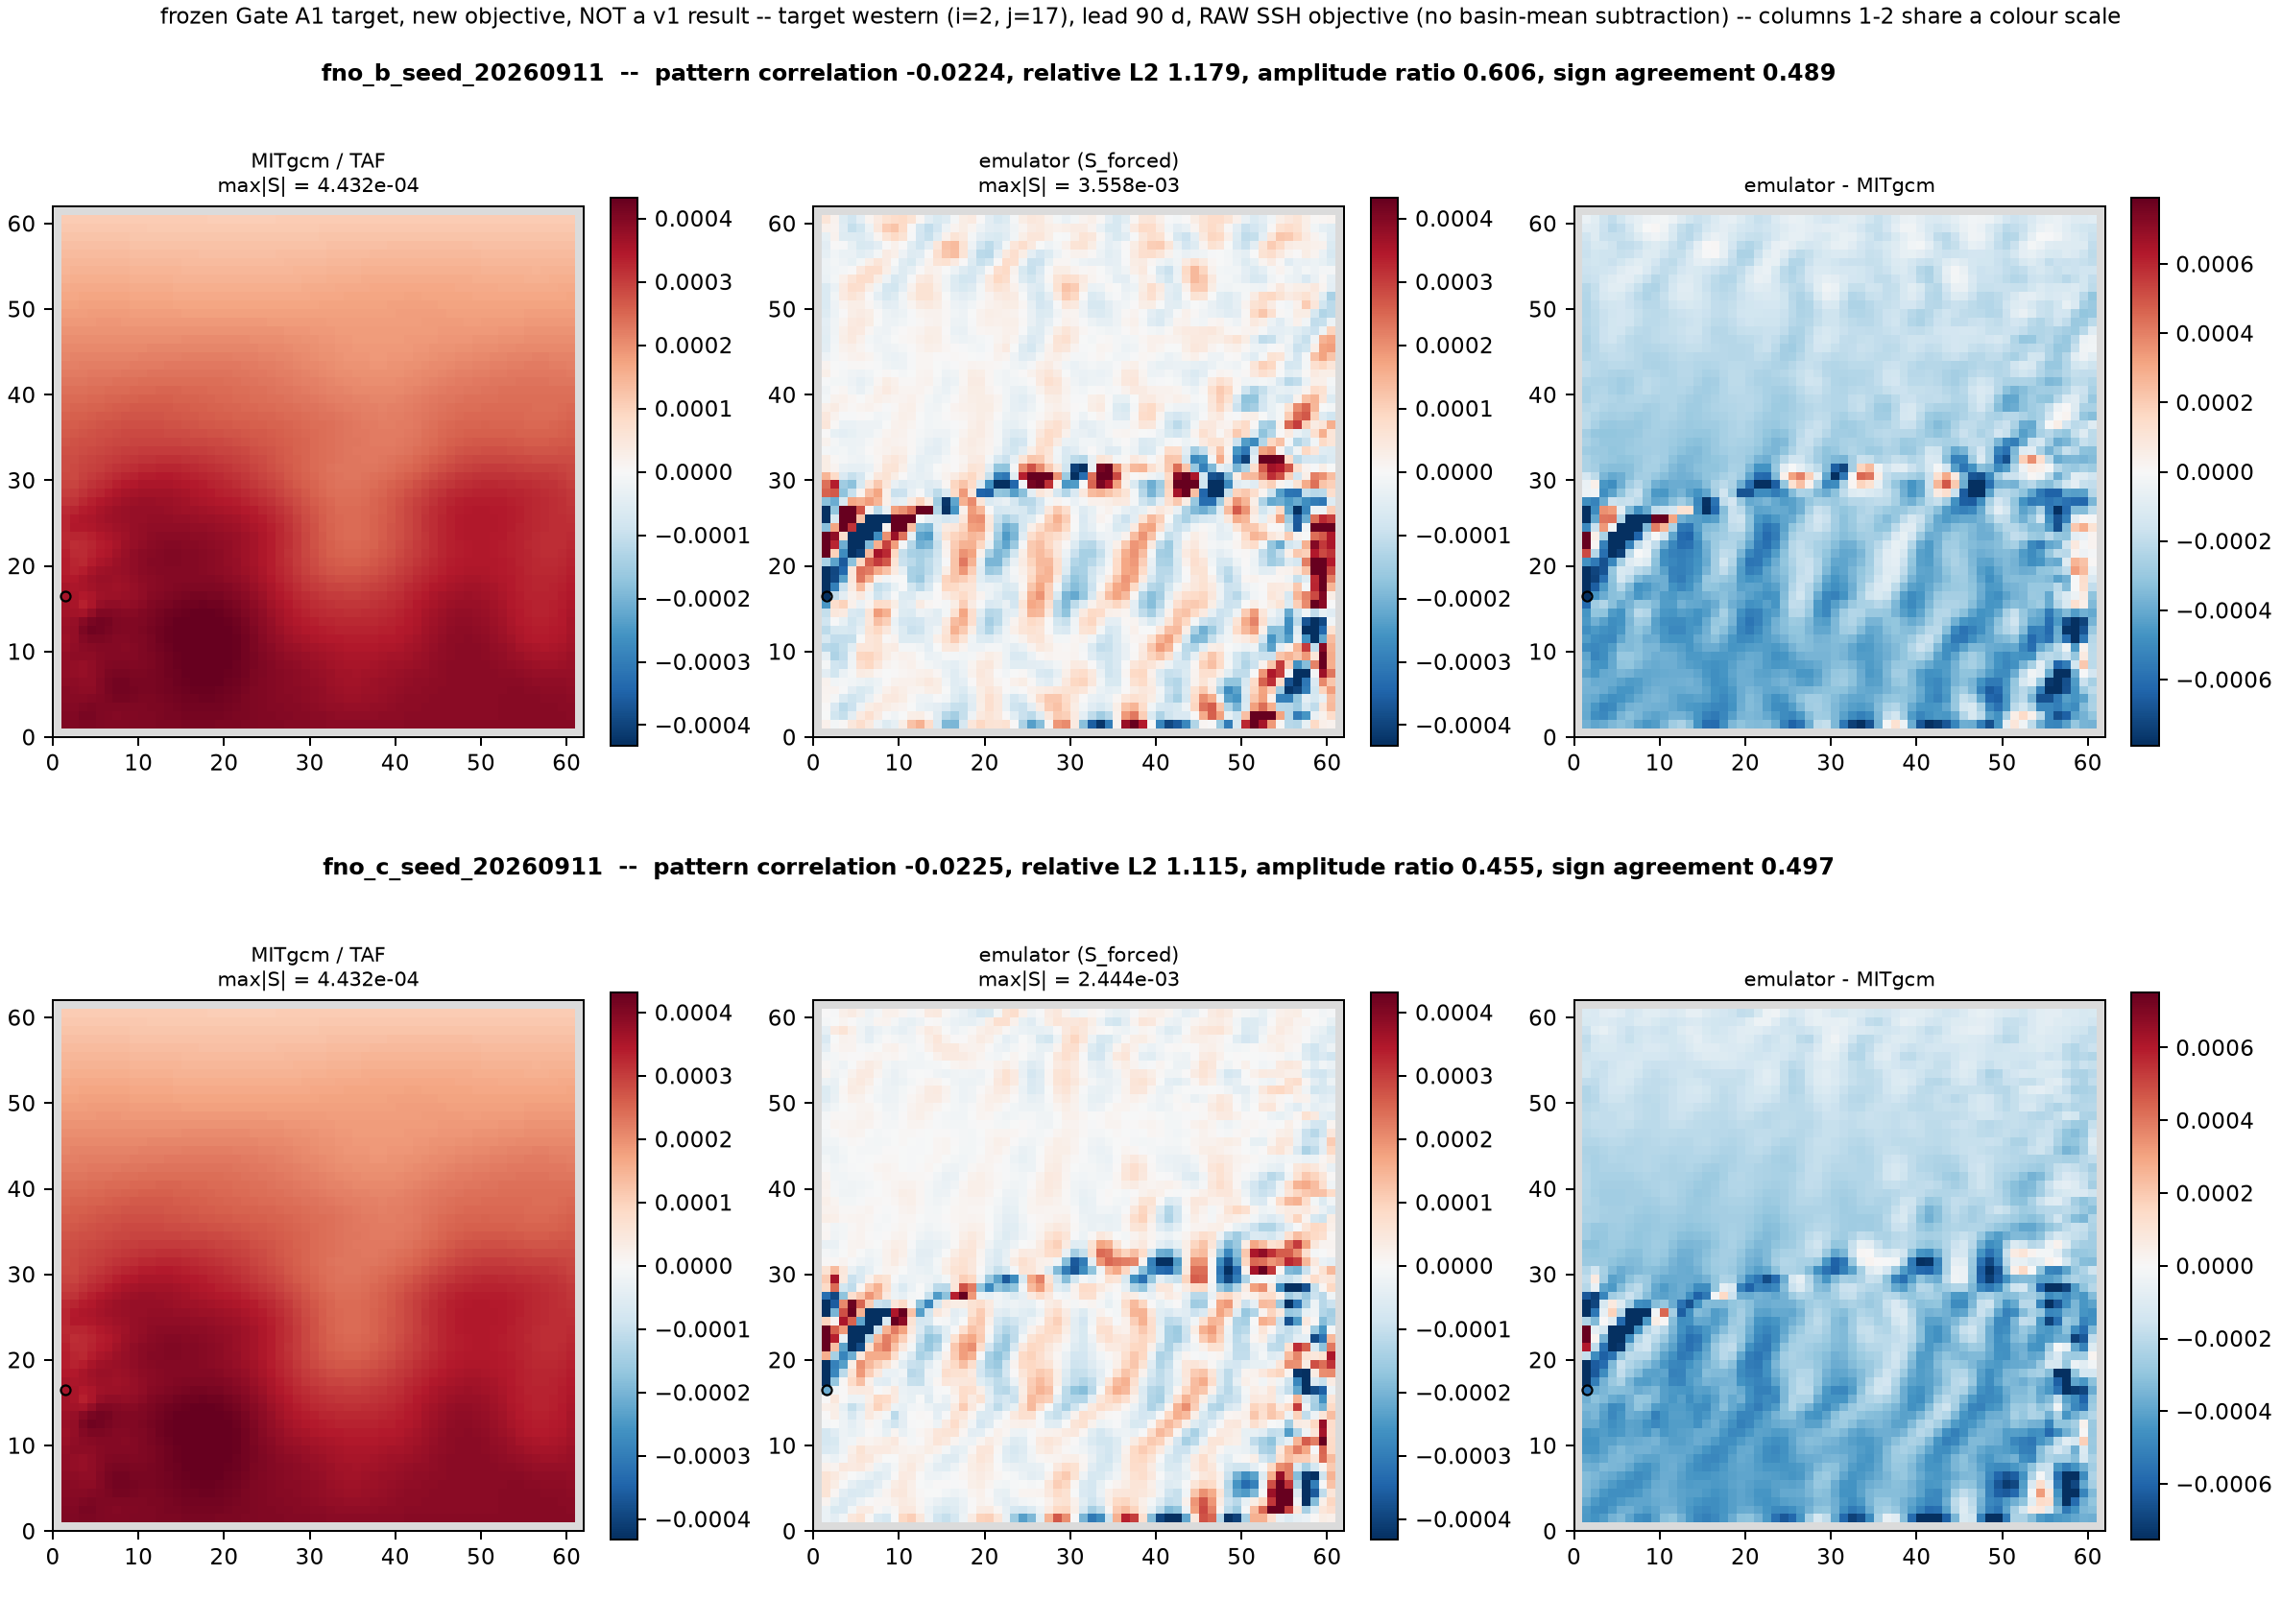
\includegraphics[width=\textwidth]{figures/adj_western_raw_ssh_090.png}
\caption{Western target, $J_{\mathrm{raw}}$, lead 90~d.}
\label{fig:west_raw090}
\end{figure}

\begin{figure}[htbp]
\centering
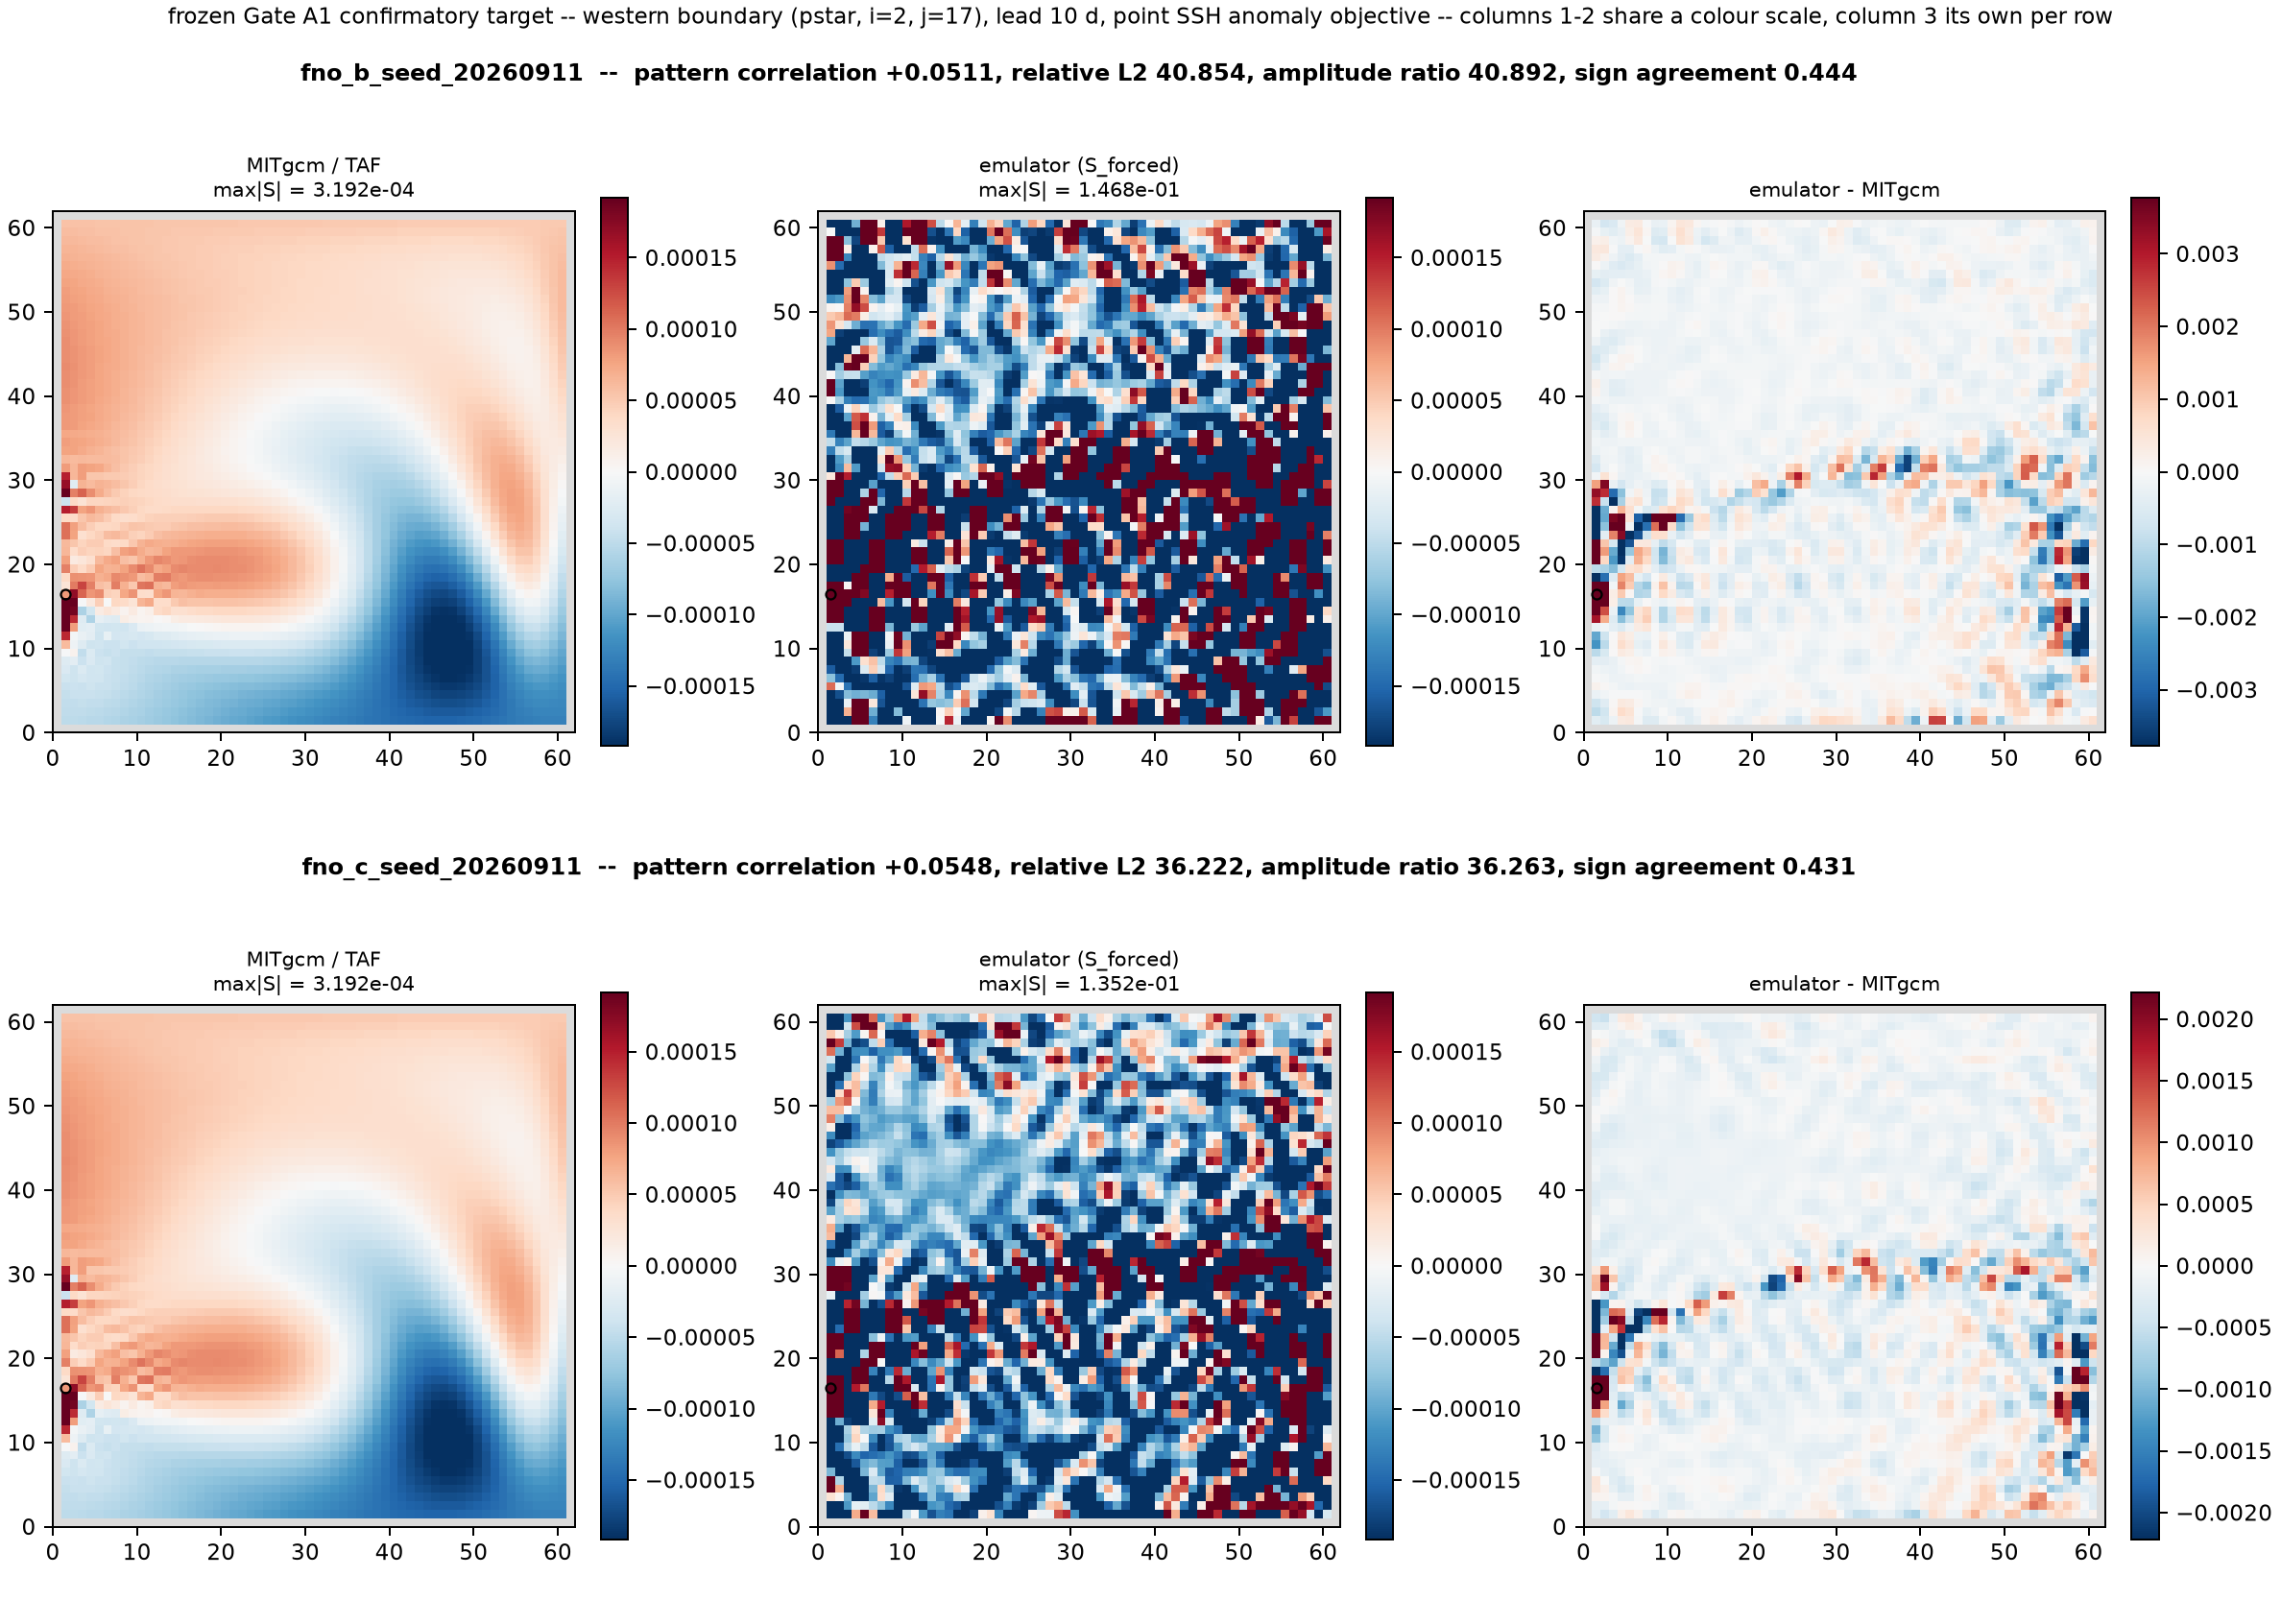
\includegraphics[width=\textwidth]{figures/adj_western_ssh_anomaly_010.png}
\caption{Western target, $J_{\mathrm{anom}}$, lead 10~d --- the study's
confirmatory cell. On a shared colour scale the reference is smooth and
organized while both emulator maps are saturated grid-scale noise, 460$\times$
too large at the peak.}
\label{fig:west_anom010}
\end{figure}

\begin{figure}[htbp]
\centering
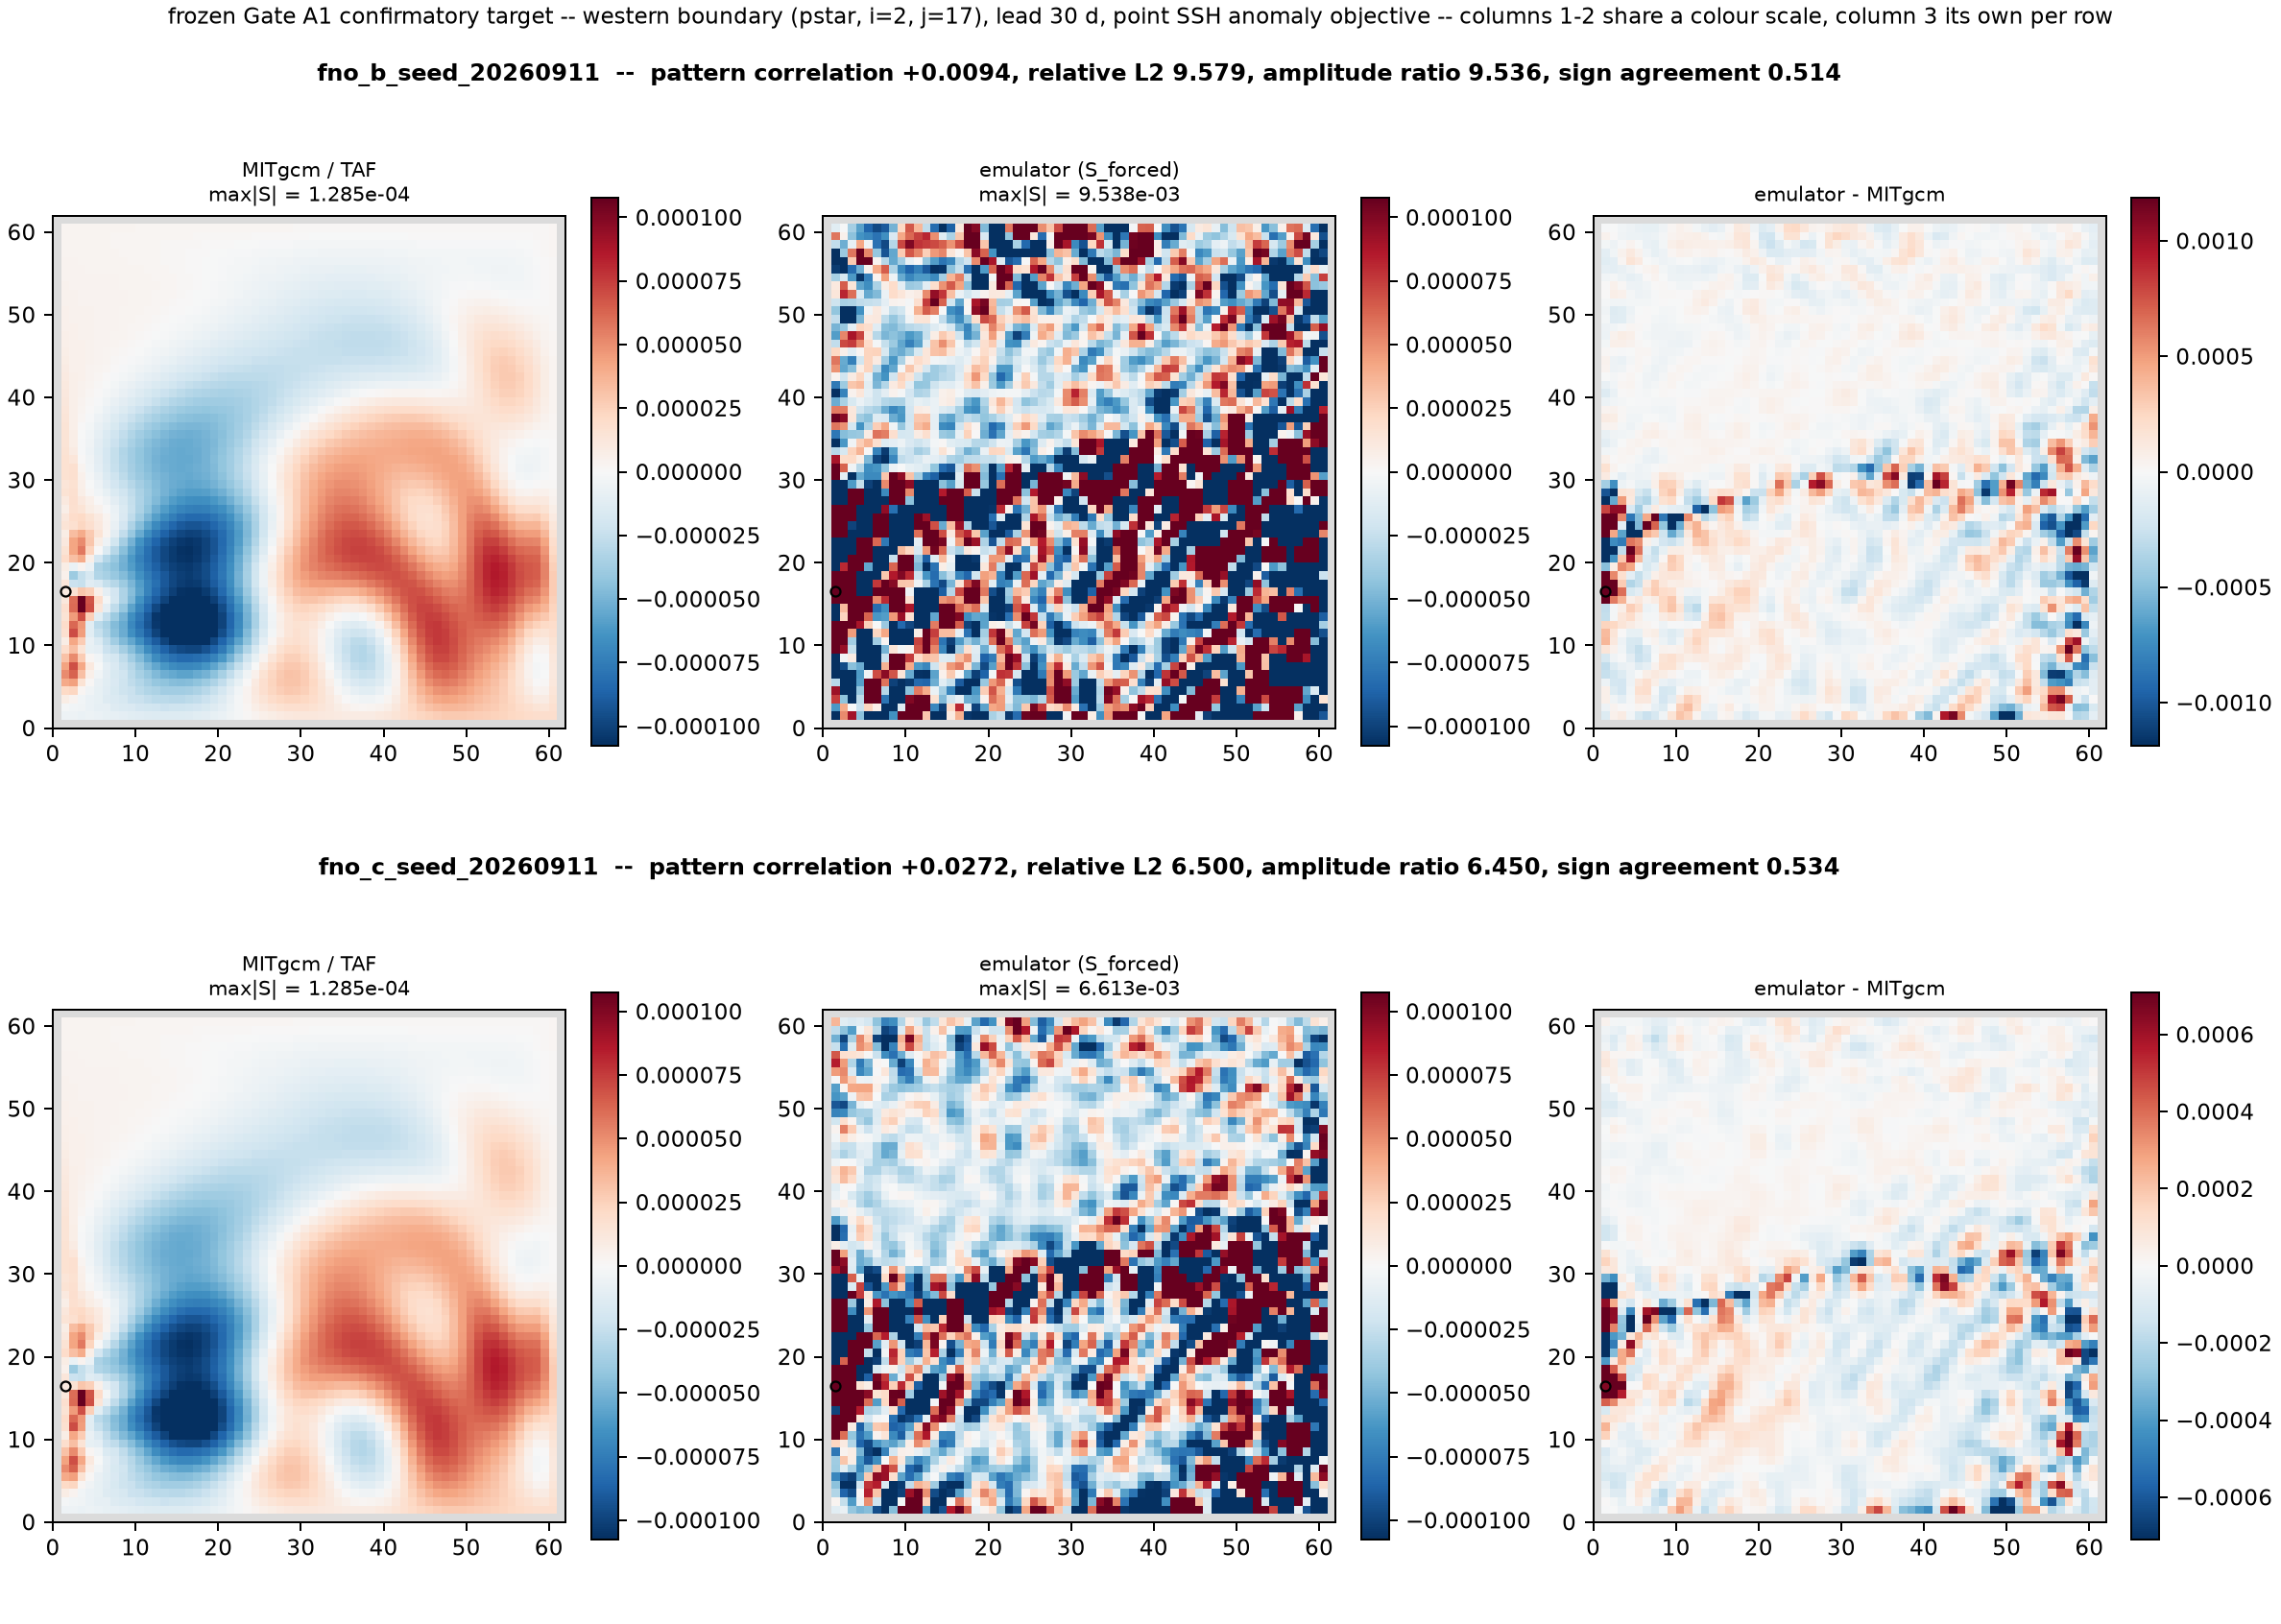
\includegraphics[width=\textwidth]{figures/adj_western_ssh_anomaly_030.png}
\caption{Western target, $J_{\mathrm{anom}}$, lead 30~d. The largest single
relative-$L_2$ reduction from the response term (9.58 $\to$ 6.50, 32\%), with
pattern correlation still at $+0.03$.}
\label{fig:west_anom030}
\end{figure}

\begin{figure}[htbp]
\centering
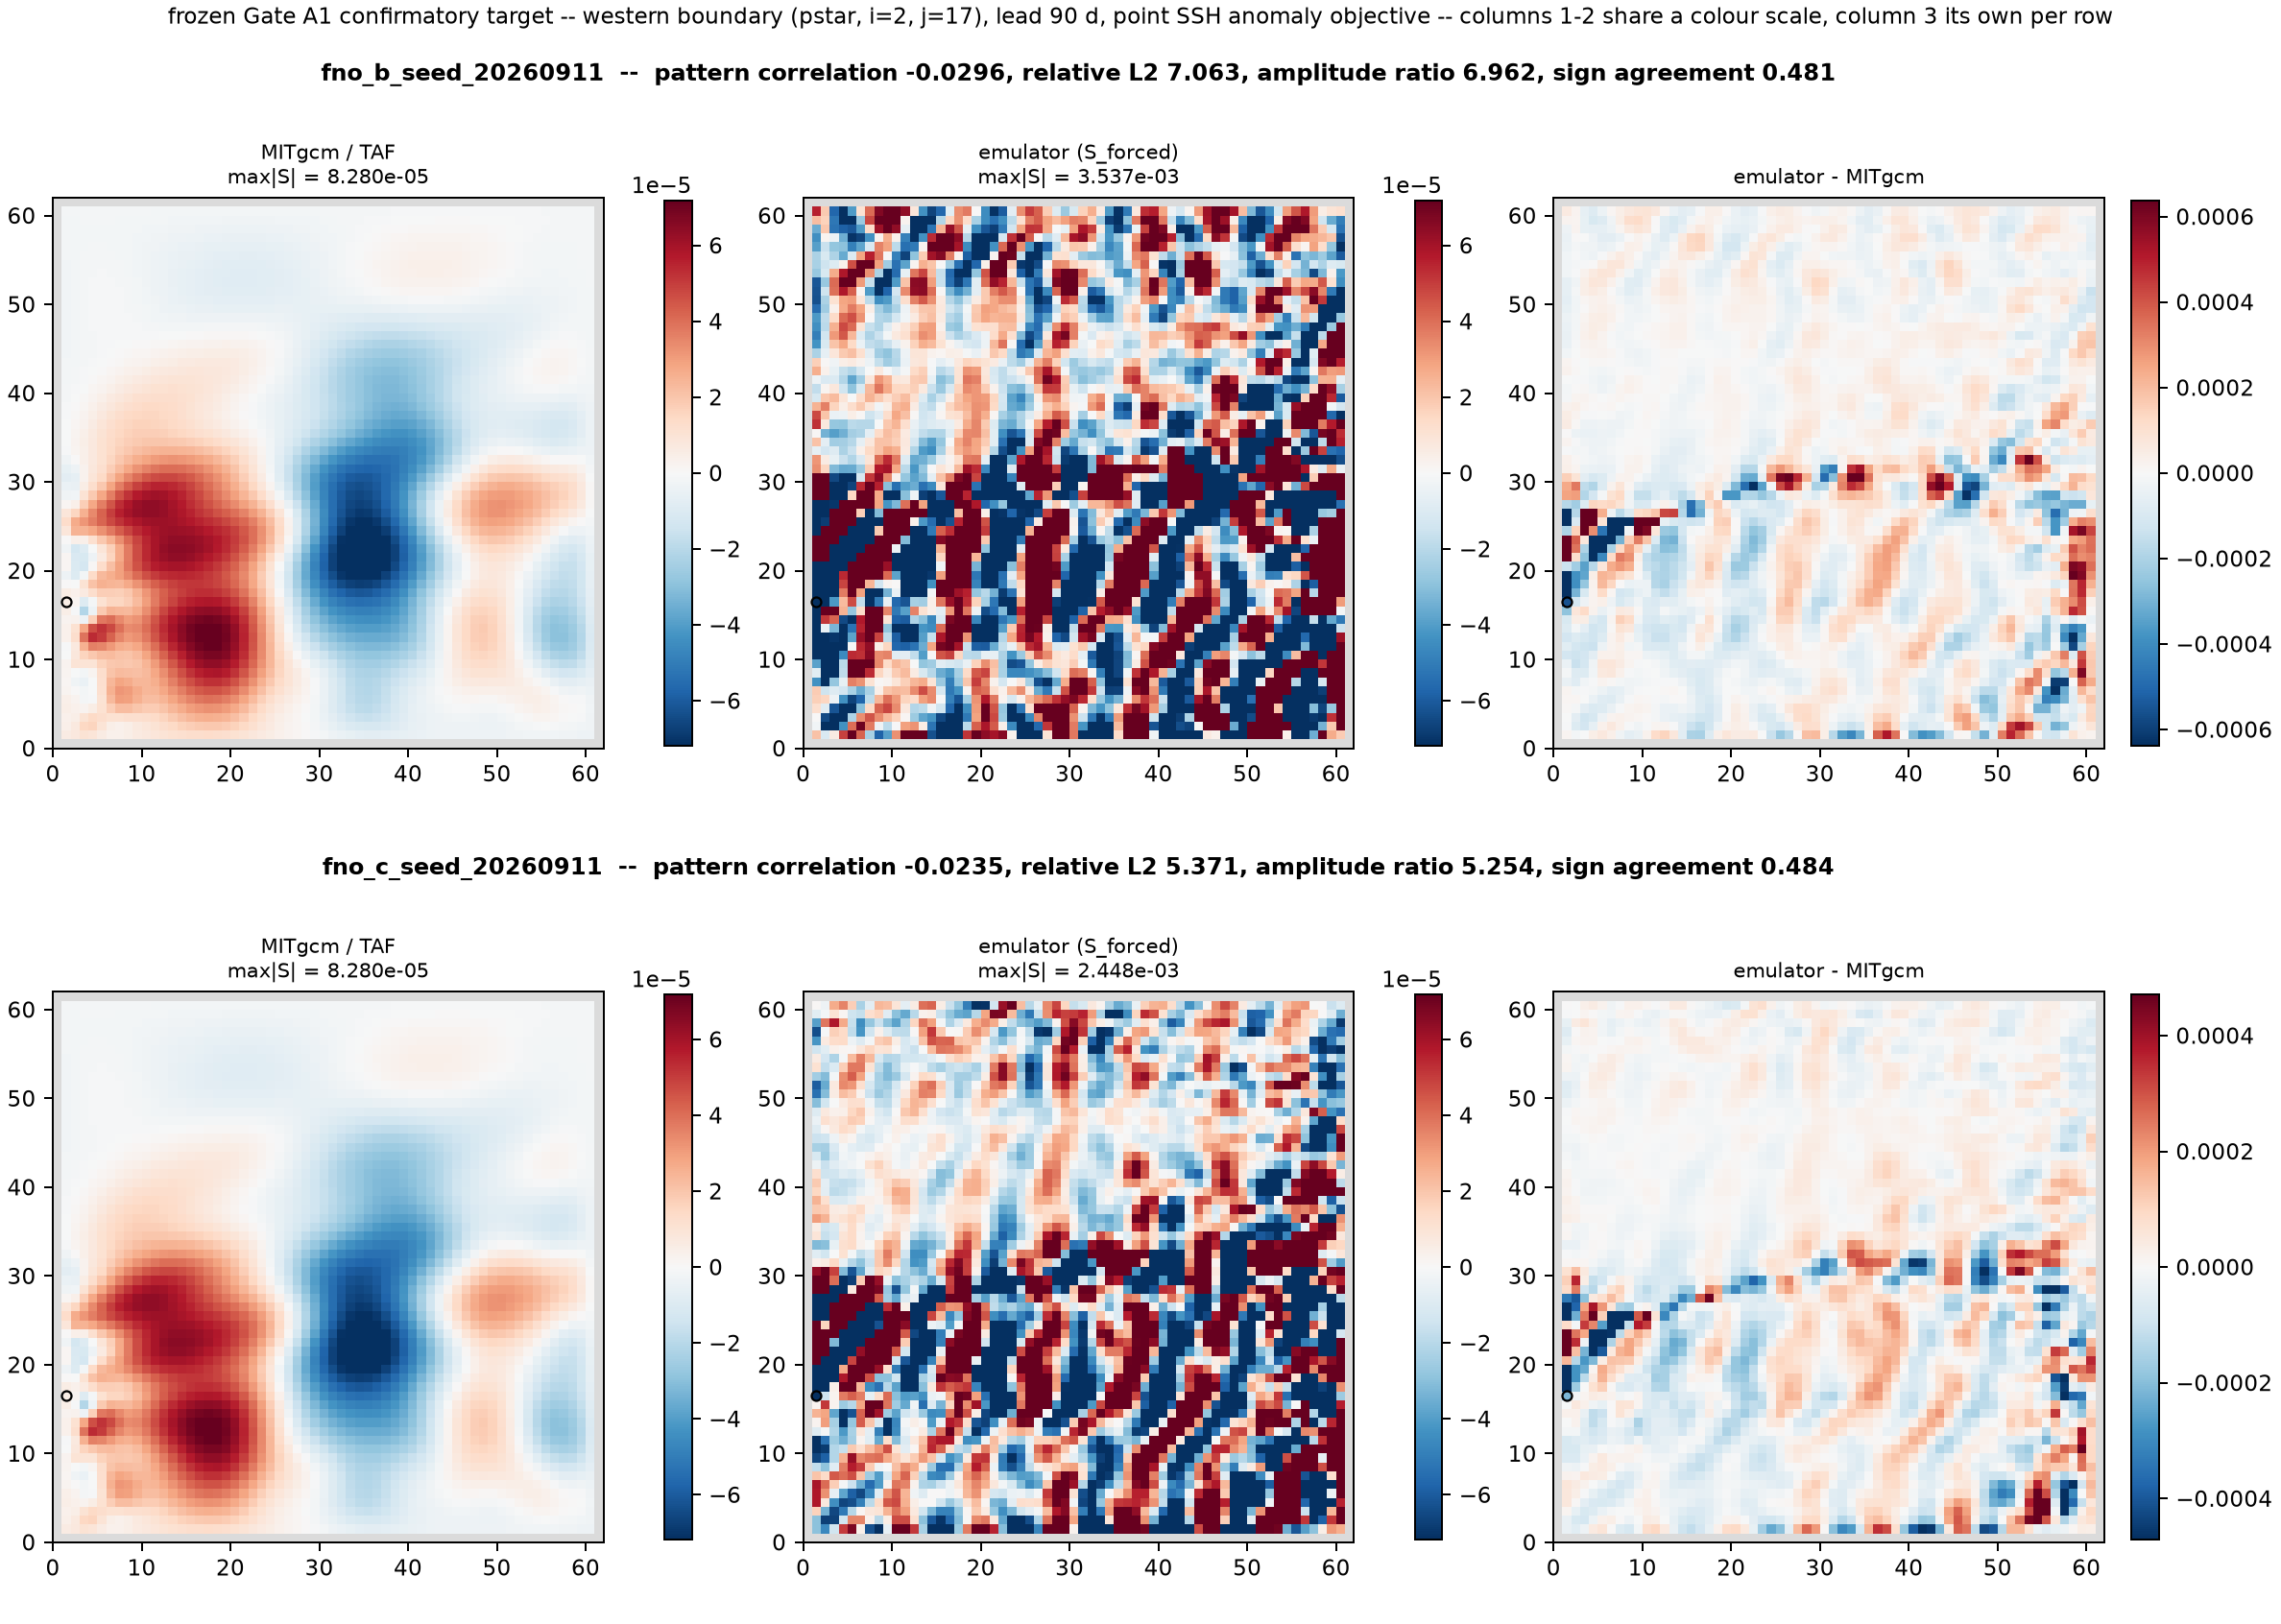
\includegraphics[width=\textwidth]{figures/adj_western_ssh_anomaly_090.png}
\caption{Western target, $J_{\mathrm{anom}}$, lead 90~d. \MITgcm{}'s adjoint has
organized into meridionally elongated Rossby lobes; both emulators show a
diagonal-striped checkerboard, still 5--7$\times$ too large.}
\label{fig:west_anom090}
\end{figure}

\section{Discussion}
\label{sec:discussion}

Three findings follow from Section~\ref{sec:results}, and they point in different
directions.

\paragraph{The response term works, in the sense it was designed to work}
Relative $L_2$ falls in all 18 (target, objective, lead) cells of
Tables~\ref{tab:interior}--\ref{tab:western}, by up to 32\%. That consistency is
not noise: the two arms share seed, data, split, schedule and every loss term but
one, so the sign of the difference is attributable to $L_{\mathrm{response}}$.
The study's pre-registered blind endpoint, computed on all three seeds before
this report, agrees --- relative $L_2$ fell in 24 of 24 confirmatory cells, with
a median ratio of 0.745, and for seed 20260911 specifically the aggregate
improvement was $\Delta_B$ ratio $0.743$, comfortably inside the pre-declared
$\le0.8$ threshold. The gate nonetheless returned \emph{negative}, because it is
judged on the pre-declared primary seed 20260724, whose $\Delta_B$ ratio was
$0.837$. Five of the six gate criteria passed. Reporting seed 20260911 here does
not change that verdict and is not intended to; it changes only which pair of
models the figures show.

\paragraph{But it corrects magnitude, not structure} Pattern correlation is the
metric the response term was supposed to move, and it does not move: across all
18 cells it stays between $-0.15$ and $+0.18$ for the control arm and between
$-0.03$ and $+0.18$ for the response arm, with no systematic difference. Every
improvement in Tables~\ref{tab:interior}--\ref{tab:western} is an amplitude
improvement, and in several cells --- eastern $J_{\mathrm{anom}}$ at lead 90 is
the clearest --- the response arm improves $\varepsilon_2$ by moving $\alpha$
\emph{away} from 1, i.e.\ by producing a smaller wrong answer. The duality
argument of Eq.~\eqref{eq:duality} explains why this is possible: matching
forward responses along a sampled set of directions constrains the adjoint's
projection onto that span, and with 672 directions in a state space of
$46\times62\times62\approx1.8\times10^{5}$ dimensions, the span is a vanishing
fraction of the whole. What the loss can cheaply satisfy is the overall scale of
the response; what it cannot reach is the geometry of the Jacobian in the
$\sim10^{5}$ unsampled directions, which is what pattern correlation measures.

\paragraph{The failure has a consistent physical shape} Across every target and
objective, the emulator's ten-day sensitivity is a near-delta at the target cell
plus grid-scale speckle along the jet axis and against the walls, whereas
\MITgcm{}'s is already basin-wide at ten days. That is the signature of an
operator whose derivative is close to the identity: an excellent forecast rule
for a slowly evolving ocean, and a wrong one for a basin in which barotropic
adjustment crosses the domain in days. That gap is not a resolution limit of
the ten-day step itself --- \MITgcm{}'s own adjoint reaches the whole basin
within one such interval, and a spectral operator does not need a signal to
physically cross the grid the way a local stencil would, since each retained
Fourier mode already couples every grid point in a single application. The more
likely explanation is architectural. Of the operations that make up each block
--- a per-mode spectral convolution, a linear channel-mixing term applied
identically at every grid point, a channel-wise multilayer perceptron, and
pointwise layer normalization --- only the spectral convolution can connect two
different grid cells at all; the rest, together with the lifting and
projection layers bracketing the three blocks, act independently at each point
and so can only ever contribute to the map's response at its own cell, never
to its spread. The bias-free local correction added at the end is local by
construction, coupling each cell only to its immediate few neighbours. A
derivative built mostly from these pointwise and local pieces, with the
spectral path's low-wavenumber content weighing in only weakly, is exactly a
near-delta with a narrow high-wavenumber halo --- which is what is observed. A
related diagnostic on this project's production checkpoint, which shares this
architecture, is consistent with that picture without establishing it for the
two arms studied here: halving the local correction's magnitude at inference
cut the long-horizon spurious anomaly's high-wavenumber power 24-fold, at a
cost of 3.9-fold worse short-lead surface-pressure error --- evidence that this
one pathway carries a large share of both the short-lead skill and the
long-horizon artefact. Nothing in the eight-term forecast objective constrains
which pathway carries the derivative, since it never evaluates the derivative
at all and rewards a near-persistent map cheaply at short lead, so training has
no reason to shape the one pathway capable of the smooth, basin-wide coupling
\MITgcm{}'s adjoint shows; forward response data supervised at the same
ten-day cadence inherits that same blindness. The mean-conservation
result (Section~\ref{sec:mean}) is the counterpart at the other extreme: a mode
with true amplification exactly 1 is damped by a near-constant $0.38$ per call,
which is exactly what a stability regularizer designed to prevent autoregressive
blow-up will do to a neutral mode. Both emulators are simultaneously far too
sensitive at high wavenumber and far too damped at the largest scale.

\paragraph{Forward cost} The response term is not free. On this seed, at day
2{,}000 the response arm's error exceeds climatology in all three primary fields
while the control arm's does not, its worst-case normalized amplitude rises from
6.55 to 9.89 (past the declared ceiling of 8), and its member spread at day
2{,}000 widens by more than an order of magnitude. Across the three seeds the
sign of the paired forward difference flips, so this is not a systematic
degradation attributable to $L_{\mathrm{response}}$ --- seed-to-seed variance in
long-rollout behaviour is larger than the treatment effect. That variance is
itself the more important observation: a training recipe whose day-2{,}000
climatology ratio ranges from 0.22 to 5.79 across three seeds is not yet
controlling the property it needs to control, and no adjoint-fidelity conclusion
drawn from a single seed of such a recipe would be safe. It is the reason the
study's frozen contract requires three paired seeds and forbids selecting a best
one.

\section{Conclusion}
\label{sec:conclusion}

A matched pair of \FNO{} emulators, identical except for one added
forward-perturbation-response loss term, was trained on the weakly turbulent S0
double gyre and compared both forward and against \MITgcm{}/TAF adjoint
sensitivities at three targets, two cost functionals and three leads. Forward,
the two arms follow the same evolution to roughly day 700 and then separate, with the
control arm remaining below climatology to day 2{,}000 on this seed and the
response arm crossing it. In the adjoint, the response term reduces the
sensitivity error consistently --- relative $L_2$ falls in every cell measured,
by up to 32\% --- but leaves pattern correlation flat near zero everywhere. The
emulator's ten-day Jacobian remains near-identity plus grid-scale noise where the
true one is already basin-wide, and both arms damp the exactly conserved
basin-mean sea-level mode by a factor of $\approx0.38$ per ten-day call.

The conclusion is that matching forward response magnitudes is insufficient to
recover adjoint structure. A response loss over a few hundred sampled directions
constrains the Jacobian's projection onto that span, and the scale of the
response is the cheapest way to satisfy that constraint; the geometry of the
operator in the remaining $\sim10^{5}$ directions is untouched. A direct
follow-up should first separate each trained model's ten-day raw-SSH sensitivity
into the contributions of the external $3\times3$ local branch and the Fourier
backbone, evaluated at the same \MITgcm{} state. This diagnostic would test
whether removing the local contribution improves spatial agreement with the
reference adjoint, rather than merely reducing sensitivity amplitude. The next
controlled experiment would retrain both the control and response models without
the $3\times3$ branch, keeping each arm's data, losses, training schedule and
budget matched to its original counterpart. Retraining would allow the backbone
to compensate for the removed branch. Evaluation against independent
\MITgcm{}/TAF adjoints should assess spatial structure, sign, amplitude and
mean-mode conservation, alongside forward accuracy and long-rollout stability.
If the backbone alone retains the poor sensitivity structure, removing the local
branch will be insufficient. This comparison should use multiple paired seeds
under a new pre-registered cycle, so that any improvement can be distinguished
from the substantial seed-to-seed variation documented here.

\section*{Data Availability}
\label{sec:data-availability}

The code, configurations and selected figures for both models discussed in
this report are available at
\url{https://github.com/m-jalabert/adjoint-faithful-fno}. Both the control
model (arm B, \texttt{model\_c\_adjoint\_faithful\_nominal\_control\_v1}) and
the response model (arm C, \texttt{model\_c\_adjoint\_faithful\_response\_v1})
are available on the \texttt{main} branch. The former
\texttt{adjoint-faithful-response-training-v1} branch has been incorporated
into \texttt{main} and removed. Commit
\texttt{94137c39fa8aca62a7345f816f0a0b33f12e84cd} records the code and
configurations used by this report and provides a fixed reference for
reproduction. Raw \MITgcm{} trajectories, restart pickups, processed datasets
and trained checkpoints are stored separately on HPC scratch and are not
included in Git. Readers must regenerate the trajectories and train the
models, or obtain those artifacts separately. The repository's
\texttt{docs/ADJOINT\_HANDOVER.md} describes the required environment,
data regeneration, training and evaluation steps.

\bibliographystyle{elsarticle-num}
\bibliography{references}

\appendix

\section{Verifying the two sensitivity pipelines}
\label{app:trust}

This appendix describes how each of the two sensitivity maps compared in
Section~\ref{sec:adjoint} is produced and independently checked, for a reader
who did not write either pipeline and wants to know what stands behind a
number in Tables~\ref{tab:mean}--\ref{tab:western} before trusting it.

\subsection{$S_{\mathrm{forced}}$ versus $S_{\mathrm{free}}$: which state the Jacobian is evaluated at}
\label{app:forced-free}

Both variants are built from the identical trained one-step Jacobian
$DF_\theta$ and the identical reverse-mode machinery; they differ only in
which states the interior links of the chain rule are evaluated at, not in
how the derivative is computed.

Write $x_0$ for the shared true initial state at day 7200, $x_1^M,\dots,x_k^M$
for \MITgcm{}'s true states at the following ten-day steps, and $x_0^F=x_0$,
$x_{j+1}^F=F_\theta(x_j^F)$ for the emulator's own autoregressive iterates.
Because the cost is linear in the final state, $J(x_k)=w\cdot x_k[\eta]$, the
seed $\nabla_{x_k}J$ does not depend on $x_0$, and reverse accumulation
through the $k$-fold composition $F_{\theta,k}=F_\theta\circ\cdots\circ
F_\theta$ gives a product of $k$ one-step Jacobian transposes,
\begin{equation}
\frac{\partial J}{\partial x_0} \;=\;
DF_\theta(x_0)^{\mathsf T}\,DF_\theta(x_1)^{\mathsf T}\cdots
DF_\theta(x_{k-1})^{\mathsf T}\,\nabla_{x_k}J.
\label{eq:chain-product}
\end{equation}
The only freedom left in Eq.~\eqref{eq:chain-product} is which states
$x_1,\dots,x_{k-1}$ the $k-1$ interior factors sit at, and $\Sforced$ and
$S_{\mathrm{free}}$ answer that differently.

\begin{equation}
S_{\mathrm{free}} \;=\;
DF_\theta(x_0^F)^{\mathsf T}\,DF_\theta(x_1^F)^{\mathsf T}\cdots
DF_\theta(x_{k-1}^F)^{\mathsf T}\,\nabla_{x_k}J,
\qquad x_{j+1}^F = F_\theta(x_j^F),
\label{eq:sfree}
\end{equation}
evaluated along the emulator's own forecast, is exactly
$DF_{\theta,k}(x_0)^{\mathsf T}\nabla_{x_k}J$ --- the true total derivative of
the deployed $k$-step autoregressive map, because $x_j^F$ really is what
$F_\theta$ produces at step $j$. This is \texttt{free\_chain}: one forward
rollout, then a single \texttt{torch.autograd.grad} call through the whole
composed graph.

\begin{equation}
S_{\mathrm{forced}} \;=\;
DF_\theta(x_0^M)^{\mathsf T}\,DF_\theta(x_1^M)^{\mathsf T}\cdots
DF_\theta(x_{k-1}^M)^{\mathsf T}\,\nabla_{x_k}J,
\label{eq:sforced}
\end{equation}
where $x_j^M$ is \MITgcm{}'s own true state at step $j$, supplied externally
at every step rather than generated by iterating $F_\theta$. This is not the
Jacobian of any single map that could be evaluated forward --- one cannot
autoregress ``on truth'' without external correction at every step --- it is
$k$ independently evaluated one-step Jacobians of $F_\theta$, chained by
matrix multiplication exactly the way \MITgcm{}'s own adjoint chains $k$
one-step Jacobians of the true dynamics along the true trajectory: TAF
linearizes the nonlinear model about its own nonlinear forward trajectory at
every timestep, by definition of an adjoint. This is \texttt{forced\_chain}:
$k$ separate \texttt{torch.autograd.grad} calls, one per step, each seeded
from the archived truth state rather than from the previous step's emulator
output.

$F_\theta$ is a nonlinear operator, so $DF_\theta$ genuinely depends on where
it is evaluated: $DF_\theta(x_j^F)\neq DF_\theta(x_j^M)$ whenever
$x_j^F\neq x_j^M$. Since the emulator's own forecast drifts from \MITgcm{}
truth as $j$ grows --- exactly the forward RMSE of Table~\ref{tab:forward} ---
the interior factors in Eqs.~\eqref{eq:sfree}--\eqref{eq:sforced} are
evaluated at increasingly different points for $k\ge2$, and
\begin{equation}
S_{\mathrm{forced}} - S_{\mathrm{free}} \;=\;
\Big[\textstyle\prod_{j} DF_\theta(x_j^M)^{\mathsf T}
- \prod_{j} DF_\theta(x_j^F)^{\mathsf T}\Big]\,\nabla_{x_k}J
\label{eq:forced-free-gap}
\end{equation}
is a direct measure of that trajectory divergence propagated through $k-1$
Jacobian factors, not a difference in how either side's derivative is
computed. At $k=1$ (lead 10) there is a single factor and $x_0^F=x_0^M=x_0$
trivially, so the two are identical bit for bit --- that identity is the
third check in Section~\ref{app:trust-fno}, below. The fraction-of-a-percent
agreement reported in Section~\ref{sec:setup} at this study's leads is the
empirical statement that trajectory error stays small relative to Jacobian
error here: most of the disagreement against \MITgcm{} in
Section~\ref{sec:adjoint} is $DF_\theta\neq DM$, not $x^F\neq x^M$.

\subsection{The \MITgcm{}/TAF reference adjoint}
\label{app:trust-mitgcm}

\MITgcm{}'s adjoint is not approximated or hand-derived: it is produced by
TAF (Transformation of Algorithms in Fortran, FastOpt), a source-to-source
automatic-differentiation tool that differentiates the model's own Fortran in
reverse mode. The differentiation itself is a single step inside
\texttt{slurm/mitgcm/af\_s0\_adjoint\_build.sbatch}: \texttt{make adall}
invokes \texttt{staf}, which submits the preprocessed forward source,
\texttt{ad\_input\_code.f}, to FastOpt's server and receives back the adjoint
source, \texttt{ad\_input\_code\_ad.f}. Every step before that is ordinary
C-preprocessing and \texttt{genmake2} configuration; every step after it is an
ordinary \texttt{gfortran} compile. \texttt{af\_fno/mitgcm/input\_ad/data.autodiff}
requests the exact adjoint (\texttt{inAdExact = .TRUE.}), with no divided or
approximate variant.

The control variable --- the quantity the adjoint is taken with respect to
--- is the initial sea surface height, wired through
\texttt{ALLOW\_GENARR2D\_CONTROL} in
\texttt{af\_fno/mitgcm/code\_ad/\allowbreak CTRL\_OPTIONS.h} and configured in
\texttt{af\_fno/mitgcm/input\_ad/data.ctrl}. This checkout's alternative,
\texttt{ALLOW\_ETAN0\_CONTROL}, compiles but is dead code --- its
implementation sits entirely inside a preprocessor guard that nothing in this
build defines --- so it silently returns a gradient of exactly zero; the live
path is confirmed never to regress to it. The cost functional itself,
$J=\sum_{ij} w_{ij}\,\eta_{ij}(T)$, is defined in
\texttt{af\_fno/mitgcm/code\_ad/cost\_test.F}, with the weight field $w$ read
as an ordinary constant, not a control, from a run-time \texttt{costWeight.bin},
wired in \texttt{af\_fno/mitgcm/input\_ad/data.cost}. The trajectory the
adjoint is linearized about is staged by \texttt{scripts/stage\_adjoint\_run.py},
whose physics namelists are identical to the renderer that produced every
forward training segment; only the run's start iteration and dump frequency
differ. The reverse sweep's own memory management --- how TAF checkpoints the
forward trajectory so it can be replayed backward without storing every
timestep --- is configured in \texttt{af\_fno/mitgcm/code\_ad/tamc.h} and is
sized to cover the full window used in this report.

Trusting the resulting gradient rests on four independent checks, all run
after the build and before any number in Section~\ref{sec:adjoint} is
produced. First, a direct finite-difference test: the control is perturbed by
$\pm\epsilon$ at a chosen cell, the forward model is run twice, and the
centred difference is compared against the adjoint's value at that cell,
swept over $\epsilon\in\{10^{-3},\dots,10^{-6}\}$ so that agreement is judged
by whether the error shrinks and then plateaus across four orders of
magnitude rather than by a single favourable epsilon. This is configured in
\texttt{af\_fno/mitgcm/input\_ad/data.grdchk} and run by
\texttt{slurm/mitgcm/af\_s0\_adjoint\_grdchk.sbatch}, which sweeps every
target cell used in this study plus points along the western boundary current
and one offshore point; the achievable precision is set by the pressure
solver's own convergence tolerance (\texttt{cg2dTargetResidual}$=10^{-7}$,
identical to every forward S0 segment), not by any looseness in the adjoint
itself. Second, \texttt{scripts/extract\_mitgcm\_adjoint.py} checks internal
consistency: the twenty-day run's adjoint state at day 7210 must equal the
independently produced ten-day run's map; the returned sensitivity must be
exactly zero on all 244 land cells and finite everywhere; and the cost value
the model itself prints must equal an independently computed
$\sum w_{ij}\eta_{ij}$ in NumPy. Third, the same script checks the one case
whose answer is known analytically: with the cost set to the pure
area-weighted mean of $\eta$, the returned sensitivity must equal the weight
field itself at every lead, because this configuration's implicit free
surface with \texttt{exactConserv} conserves that mean exactly --- a case
with no free parameters to tune and no room for the two sides to agree by
coincidence. Fourth, every downstream extraction records the SHA-256 of the
executable that produced it, so a later run using a different build --- a
different TAF submission, a different compiler flag --- is caught rather than
silently mixed into the same dataset.

\texttt{tests/test\_mitgcm\_adjoint.py} encodes the compile-time and namelist
half of all of this as ordinary tests --- which preprocessor flags must be
defined, which must not, the tile-local indexing that
\texttt{af\_s0\_adjoint\_grdchk.sbatch} depends on, the checkpoint budget in
\texttt{tamc.h} --- runnable without \MITgcm{}, TAF or a GPU, so a change to
the build configuration that would silently break the adjoint fails in
continuous testing before it ever reaches a cluster job.

\subsection{The \FNO{} emulator's reverse-mode gradient}
\label{app:trust-fno}

The emulator side needs no separate adjoint code: \texttt{S\_forced} and
\texttt{S\_free} are produced by ordinary reverse-mode automatic
differentiation (PyTorch \texttt{autograd}) through the same trained network
used for forecasting, implemented in \texttt{scripts/fno\_adjoint\_ft90.py}.
\texttt{scripts/fno\_adjoint\_model.py} is a thin registry over that one
script --- which checkpoint, which report, which output directory --- used
identically for the frozen parent model and for every paired control/response
replicate in this study, so the same differentiation machinery produces every
map compared in this report.

Trust here starts with knowing that the thing being differentiated is exactly
the thing that was deployed. \texttt{load\_frozen\_model} loads the published
checkpoint with strict key matching, asserts the loaded parameter count
against the value recorded when the checkpoint was written, and freezes every
weight; a companion check then walks every module confirming that no
training-time hook, parametrization or spectral-norm estimator buffer is
still attached to the loaded network, since any of those would mean the
differentiated map is not the one the model actually deploys.

A genuine numerical defect was found and fixed here, and is verified rather
than assumed away. The third-party spectral-convolution layer that holds
97.95\% of this architecture's parameters allocates its internal Fourier
working buffer in single precision regardless of the model's own dtype, so
casting the model to double precision left almost the entire operator's
gradient computed in float32 while every downstream report claimed float64.
\texttt{DoublePrecisionSpectralConv} in
\texttt{scripts/fno\_adjoint\_ft90.py} patches that buffer to follow the
model's precision, and \texttt{verify\_double\_precision\_spectrum} confirms
the fix took effect twice over: by directly observing the buffer's dtype
during a forward pass, and by checking the adjoint identity
$\langle v,Ju\rangle=\langle J^{\mathsf T}v,u\rangle$ on the affected layer,
which only holds to machine precision once the promotion is in place.

The Jacobian-vector products themselves are built inside
\texttt{FrozenOperator} (\texttt{scripts/\allowbreak fno\_adjoint\_ft90.py}), which places
the physical-to-normalized coordinate change and the wet-cell mask inside the
autograd graph rather than applying them by hand outside it, so reverse-mode
differentiation automatically carries every factor of the per-channel
normalization scale and returns exactly zero on land --- the same property
\MITgcm{}'s land check enforces, arrived at the same way, by construction
rather than by post-hoc correction. \texttt{S\_forced} is assembled by
chaining one vector-Jacobian product per ten-day step backward through the
\MITgcm{} truth states (\texttt{forced\_chain}); \texttt{S\_free} by one
forward pass along the emulator's own rollout followed by one backward pass
per objective (\texttt{free\_chain}).

Four checks establish that this reverse-mode gradient is correct. A
finite-difference sweep at the same eight cells and the same style of
epsilon ladder as the \MITgcm{} side, implemented in
\texttt{scripts/fno\_adjoint\_ft90.py}, plays the same role as \MITgcm{}'s own
check, with a tighter tolerance justified by the absence of any
solver-tolerance or convective-adjustment discontinuity on this side. A
second, independent check computes the same directional derivatives by
forward-mode automatic differentiation (\texttt{torch.func.jvp}, in
\texttt{forward\_versus\_reverse}) --- a completely different code path,
accumulating in the opposite order, that involves no subtraction of nearly
equal numbers and is therefore not limited by the cancellation a finite
difference suffers from; agreement between the two modes to a measured
machine-precision floor is stronger evidence than any finite difference alone
can supply. A third check compares the two autoregressive chains directly: at
lead 10, \texttt{S\_forced} and \texttt{S\_free} are the same computation by
construction, and the two independent implementations are required to agree
bit-for-bit, not merely to within tolerance. A fourth check runs the same
analytically known case as the \MITgcm{} side --- the conserved basin mean ---
and reports, rather than grades, how far the emulator's answer sits from the
exact weight field at every lead; this is the check that surfaces the
$\approx0.38$-per-call damping of the one mode whose true answer is known,
discussed in Section~\ref{sec:mean}.

\texttt{tests/test\_fno\_adjoint.py} fixes the frozen contract this all
depends on --- channel indices, the day windows each experiment differentiates
over, the checkpoint's expected parameter count and hash --- as tests runnable
without a GPU, the trained checkpoint, or \MITgcm{}, so the same class of
silent drift the \MITgcm{}-side tests guard against is caught here too.

\subsection{Keeping the comparison itself honest}
\label{app:trust-shared}

Producing two independently verified sensitivity maps is not sufficient on
its own; the two must also be asking the same question. This is enforced in
code rather than left to convention: the comparison in
\texttt{scripts/compare\_adjoint\_maps.py} refuses to run unless the
\MITgcm{} side's own finite-difference check has already passed, and unless
both sides' cost-weight files hash identically and target the same grid cell
--- so a stale weight file or a silently moved target on either side fails
the comparison outright rather than producing a plausible-looking but
meaningless number. Both pipelines are required to share the same cost
functional, the same three target cells, the same sign convention (a positive
entry means raising sea level at the source raises the target), the same
physical units, and the same treatment of land, and
\texttt{scripts/adjoint\_metrics.py} applies the four comparison metrics of
Eqs.~\eqref{eq:corr}--\eqref{eq:sign} identically to both maps over the same
wet-cell mask. The one substantive modelling choice that makes the
comparison meaningful rather than merely well-typed is that \texttt{S\_forced}
--- the map actually compared to \MITgcm{} throughout Section~\ref{sec:adjoint}
--- is linearized about the true \MITgcm{} trajectory at every step, exactly
as \MITgcm{}'s own adjoint is; this is what lets a disagreement be read as
Jacobian error rather than as the two sides having quietly drifted apart onto
different trajectories.

\end{document}
